\def\SigleNumero{STT-1000}
\def\NomCours{Probabilités et statistique}

\newcommand{\affichepoints}{.}     % ← AVEC points
% \renewcommand{\affichepoints}{on} % ← SANS points (non vide)

\documentclass{Evaluation}
\usepackage{multicol,graphicx}
\usepackage{fancyvrb}
\usepackage{comment}
\noprintanswers

% Commande utilisée dans certains examens pour l'espace réponse vrai/faux
\newcommand{\vfrep}[1]{}

% ============================================================
% MÉCANISME D'AFFICHAGE CONDITIONNEL DES TITRES DE MODULES
% Le titre d'un module n'apparaît que si au moins une session
% active contient des questions dans ce module.
% ============================================================
\makeatletter
\newcommand{\currentmodulekey}{}
\newcommand{\currentmoduletitle}{}
\newcommand{\currentgroupkey}{}
\newcommand{\currentgrouptitle}{}
% \modulegroupheader{clé}{titre} — en-tête de groupe (affiché une seule fois)
\newcommand{\modulegroupheader}[2]{%
  \renewcommand{\currentgroupkey}{#1}%
  \renewcommand{\currentgrouptitle}{#2}%
  \expandafter\global\expandafter\let\csname modulegroup@#1@shown\endcsname\relax
}
% \moduleheader{clé}{titre} — enregistre le titre sans l'afficher
\newcommand{\moduleheader}[2]{%
  \renewcommand{\currentmodulekey}{#1}%
  \renewcommand{\currentmoduletitle}{#2}%
  \expandafter\global\expandafter\let\csname module@#1@shown\endcsname\relax
}
% \showmoduleifneeded — appelé au début de chaque session active
\newcommand{\showmoduleifneeded}{%
  % Afficher l'en-tête de groupe si nécessaire
  \ifx\currentgroupkey\empty\else
    \expandafter\ifx\csname modulegroup@\currentgroupkey @shown\endcsname\relax
      \section*{\currentgrouptitle}%
      \expandafter\gdef\csname modulegroup@\currentgroupkey @shown\endcsname{1}%
    \fi
  \fi
  % Afficher l'en-tête de module si nécessaire
  \expandafter\ifx\csname module@\currentmodulekey @shown\endcsname\relax
    \section*{\currentmoduletitle}%
    \expandafter\gdef\csname module@\currentmodulekey @shown\endcsname{1}%
  \fi
}
\makeatother

% ============================================================
% CONFIGURATION DES SESSIONS À AFFICHER
% Par défaut, toutes les sessions sont affichées (environnements no-op).
% Pour CACHER une session, décommentez la ligne \excludecomment correspondante.
% ============================================================
\newenvironment{A22}{\showmoduleifneeded}{}
\newenvironment{H23}{\showmoduleifneeded}{}
\newenvironment{A23}{\showmoduleifneeded}{}
\newenvironment{A24}{\showmoduleifneeded}{}
\newenvironment{H25}{\showmoduleifneeded}{}
\newenvironment{A25}{\showmoduleifneeded}{}
\newenvironment{H26}{\showmoduleifneeded}{}
\newenvironment{H26r}{\showmoduleifneeded}{}

% Décommentez les lignes ci-dessous pour cacher des sessions :
%\excludecomment{A22}
%\excludecomment{H23}
%\excludecomment{A23}
%\excludecomment{A24}
%\excludecomment{H25}
%\excludecomment{A25}
%\excludecomment{H26}
%\excludecomment{H26r}

% Supprimer la page couverture et ajuster les marges
\renewcommand{\couverture}{\newgeometry{margin=1.7cm,left=0.7cm,bottom=1.5cm,footskip=0.5cm}}

\begin{document}

\begin{center}
  {\Large\textbf{\SigleNumero\ -- \NomCours}}\\[0.3cm]
  {\large Recueil d'exercices}
\end{center}
\medskip

\begin{questions}


\moduleheader{mod1}{Module 1 - Introduction aux probabilités}

\begin{A22}
\question (A22)  Considérons le montage électronique représenté ci-dessous. 
	
	\begin{figure}[h!]
		\label{A22-I1-fig:montage}
		\begin{center}	\begin{tikzpicture}	
			
			\draw (0,0)--(1,0);
			\draw (1,0)--(1,1);
			\draw (1,0)--(1,-1);
			\draw (1,1)--(1.7,1);
			\draw (2.3,1)--(3,1);
			\draw (1,-1)--(1.7,-1);
			\draw (2.3,-1)--(3,-1);
			\node at (2,1) {A1};
			\node at (2,-1) {A2};
			\draw (3,-1)--(3,1);
			\draw (3,0)--(4,0);
			\node at (2,-1.6) {Bloc A};
			\end{tikzpicture} \end{center}
		\end{figure}
	Le bloc A contient deux éléments. Nous avons que
	\begin{itemize}
		\item L'élément A1 fonctionne avec une probabilité de 0,70.
		\item L'élément A2 fonctionne avec une probabilité de 0,70.
	\end{itemize}
	Pour que le montage fonctionne, au moins un élément du bloc A doit fonctionner. Les éléments d'un bloc fonctionnent de façon indépendante.
	
	
	

Quelle est la probabilité que le montage ne fonctionne pas? 

\begin{oneparcheckboxes}
\choice $0,49$
\choice $0,70$
\choice $0,03$
\choice $0,91$
\CorrectChoice $0,09$
\end{oneparcheckboxes}

\begin{solution}
$P(\bar{F})= P(\bar{A1}) \times P(\bar{A2}) = 1 - \left[\left\{1-P\left(\bar{A_1}\right)\right\}\left\{1-P\left(\bar{A_2}\right)\right\}\right]=1-0,3^2=0,91$
\end{solution}
\end{A22}

\begin{A22}
\question (A22)  Soit $A$ et $B$, deux événements de $S$. Nous savons que $$0<P(A)+P(B)<1.$$ Laquelle des affirmations suivantes est tout le temps vraie?

\begin{checkboxes}
    \choice $A$ et $B$ sont indépendants
    \choice $A$ et $B$ forment une partition de l'espace échantillonnal
    \correctchoice $P(A \cup B) > 0$
    \choice $P(A \cap B) > 0$
    \choice $A$ et $B$ sont mutuellement exclusifs
\end{checkboxes}

\begin{solution}
Comme $P(A)+P(B)>0$, on a que $P(A)>0$ ou $P(B)>0$.\\ 
$A \perp B$ si $P(A\cap B)=P(A)P(B)$. Nous n'avons pas suffisamment d'informations.\\
Comme $P(A)+P(B)<1$, ils ne forment pas une partition de l'espace échantillonnal.\\
Suite\\
Réponse C)
\end{solution}
\end{A22}

\begin{A22}
\question (A22)  Soit $A\subset B \subset S$ où $S$ est l'ensemble universel.\\
Laquelle des expressions suivantes est toujours vraie si $P(A)~>~0$~et~$P(B)~>~0$?

\begin{oneparcheckboxes}
    \choice $P(A) > P(B)$
    \choice $P(A)+P(B)<1$
    \correctchoice $P(A|B)\geq P(A)$
    \choice $P(B|A)=0$
\end{oneparcheckboxes}
\end{A22}

\begin{A22}
\question (A22) 
Une population est formée à 40\% d'enfants et à 60\% d'adultes. On sait que parmi les enfants 95\% aiment le chocolat, et que parmi les adultes seulement 70\% aiment le chocolat. On choisit par hasard une personne parmi celles qui aiment le chocolat. Quelle est la probabilité que celle-ci soit un enfant? Justifiez vos calculs.
\begin{solution}
Soit la notation suivante : 
E : être un enfant
A: être un adulte
C: aimer le chocolat
On sait que $P(E)=0.4$, $P(A)=0.6$, $P(C|E)=0.95$ et $P(C|A)=0.7$.
On cherche $P(E|C)$.
On doit ici utiliser le théorème de Bayes. On a donc 
\begin{align}
    P(E|C) &= \frac{P(C|E)P(E)}{P(C)}\\
    &= \frac{P(C|E)P(E)}{P(C|E)P(E) + P(C|A)P(A)} \\
    &= \frac{0.95 * 0.4}{0.95 * 0.4 + 0.7*0.6}\\
    &= \frac{0.38}{0.38+0.42} \\
    &= 0.457
\end{align}
\end{solution}
\end{A22}

\begin{A22}
\question (A22) Après un certain nombre de tours pendant une partie de \textit{Scrabble}, les 15 lettres suivantes n'ont toujours pas été choisies et sont donc encore dans le sac:
$$\{a, e, i, g, h, l, n, o, p, t, t, v, v, w, x\}.$$

\begin{parts}
    \part[4] Si Alex doit piger 4 lettres au hasard dans le sac, quelle est la probabilité que ces lettres soit les lettres de son prénom, dans le bon ordre? Laissez des traces de votre démarche.
\begin{solution}
    Soit l'événement $A:$ Alex pige les lettres de son nom dans l'ordre.
    
    Comme l'ordre est important, la probabilité est

    \begin{align*}
        P(A)&=\frac{1}{15}\times\frac{1}{14}\times\frac{1}{13}\times\frac{1}{12}\\
        P(A)&= \frac{1}{32760}
    \end{align*}
\end{solution}

     
    \part[6] Supposons qu'Alex a pigé $\{i, g, t, w\}$. Il reste donc 
$\{a, e, h, l, n, o, p, t, v, v, x\}$ dans le sac. C'est maintenant au tour d'Eva de piger 4 lettres. Quelle est la probabilité que parmi ses 4 lettres, elle pige les lettres qui forment son prénom (peu importe l'ordre)? Laissez des traces de votre démarche.
\begin{solution}
     Soit l'événement $E:$ Eva pige au moins les 3 lettres de son nom peu importe l'ordre.
    
    Comme l'ordre n'est pas important.

    \begin{align*}
        P(E)&= \frac{\binom{1}{1}\binom{1}{1}\binom{2}{1}\binom{8}{1}}{\binom{11}{4}}\\
        &= \frac{16}{330}\\
        &\approx 0,0485
    \end{align*}
\end{solution}
\end{parts}
\end{A22}

\begin{H23}
\question (H23)  Soient $A$ et $B$ deux événements de $\mathcal{U}$ tels que 
\begin{itemize}
\item $\mathbb{P}(\overline{A \cup B})=0.4$
\item $\mathbb{P}(A \cap \overline{B})=0.2$
\item $\mathbb{P}(\overline{A}\cap B)=0.1$
\end{itemize}
Calculer $\mathbb{P}(A \cap B)$.

\begin{solution}
On sait que $\mathbb{P}(\overline{A \cup B}) = 0{,}4$, donc $\mathbb{P}(A \cup B) = 1 - 0{,}4 = 0{,}6$.

Or, l'union se décompose en trois parties disjointes :
$$\mathbb{P}(A \cup B) = \mathbb{P}(A \cap \overline{B}) + \mathbb{P}(\overline{A} \cap B) + \mathbb{P}(A \cap B)$$
Donc
$$0{,}6 = 0{,}2 + 0{,}1 + \mathbb{P}(A \cap B)$$
$$\mathbb{P}(A \cap B) = 0{,}3$$
\end{solution}
\end{H23}

\begin{H23}
\question (H23)  Soient $A$, $B$ et $C$ trois événements de $\mathcal{U}$ tels que 
\begin{itemize}
\item $\mathbb{P}(A)=0.4$
\item $\mathbb{P}(B)=0.5$
\item $\mathbb{P}(C)=0.2$
\item les événements $A$ et $B$ sont indépendants
\item les événements $B$ et $C$ sont indépendants.
\item les événements $A$ et $C$ sont mutuellements exclusifs.
\end{itemize}
Calculer $\mathbb{P}(A \cup B \cup C)$.

\begin{solution}
Par la formule d'inclusion-exclusion :
$$\mathbb{P}(A \cup B \cup C) = \mathbb{P}(A) + \mathbb{P}(B) + \mathbb{P}(C) - \mathbb{P}(A \cap B) - \mathbb{P}(A \cap C) - \mathbb{P}(B \cap C) + \mathbb{P}(A \cap B \cap C)$$

\begin{itemize}
\item $A$ et $B$ indépendants : $\mathbb{P}(A \cap B) = \mathbb{P}(A)\mathbb{P}(B) = 0{,}4 \times 0{,}5 = 0{,}2$
\item $A$ et $C$ mutuellement exclusifs : $\mathbb{P}(A \cap C) = 0$
\item $B$ et $C$ indépendants : $\mathbb{P}(B \cap C) = \mathbb{P}(B)\mathbb{P}(C) = 0{,}5 \times 0{,}2 = 0{,}1$
\item $A \cap B \cap C \subseteq A \cap C = \varnothing$, donc $\mathbb{P}(A \cap B \cap C) = 0$
\end{itemize}

Ainsi,
$$\mathbb{P}(A \cup B \cup C) = 0{,}4 + 0{,}5 + 0{,}2 - 0{,}2 - 0 - 0{,}1 + 0 = 0{,}8$$
\end{solution}
\end{H23}

\begin{H23}
\question (H23)  Une association est composée de 30 personnes. De combien de façons est-ce qu'on peut former un bureau exécutif composé d'un président, un vice-président, un trésorier et 4 membres?

\begin{solution}
On choisit d'abord les 3 postes nommés (ordre important) parmi 30 personnes :
$$P^{30}_3 = 30 \times 29 \times 28 = 24\,360$$

Puis on choisit 4 membres parmi les 27 restants (sans ordre) :
$$\binom{27}{4} = \frac{27!}{4!\,23!} = 17\,550$$

Le nombre total de façons est donc :
$$24\,360 \times 17\,550 = 427\,518\,000$$
\end{solution}
\end{H23}

\begin{H23}
\question (H23)  Une usine fabrique 3 types de télévisions qu'on nomme $A$, $B$ et $C$. On nous dit que $50\%$ des télévisions fabriqués sont de type $A$ et $20\%$ de type $B$. On nous dit aussi que $5\%$ de télévisions de type $A$, $10\%$ des télévisions de type $B$ et $15\%$ des télévisions de type $C$ sont défectueuses. Quelle est la probabilité qu'une télévision défectueuse soit~de~type~$B$?

\begin{solution}
$P(A)=0,5$, $P(B)=0,2$, donc $P(C)=0,3$.

$P(D|A)=0,05$, $P(D|B)=0,1$ et $P(D|C)=0,15$.

On cherche $P(B|D)$.

\begin{align*}
    P(B|D) = & \frac{P(B\cap D)}{P(D)}\\
    =& \frac{P(D|B)P(B)}{P(D\cap A)+P(D\cap B) + P(D\cap C)}\\
    =&\frac{P(D|B)P(B)}{P(D| A)P(A)+P(D|B)P(B) + P(D| C)P(C)}\\
    =&\frac{0,1 \cdot 0,2}{0,05\cdot 0,5 + 0,1 \cdot 0,2 + 0,15 \cdot 0,3}\\
    =& \frac{0,02}{0,09}\\
    =& \frac{2}{9}
\end{align*}
\end{solution}
\end{H23}

\begin{A23}
\question (A23) \label{A23-I3-probaQCM} Considérons le montage électronique représenté ci-dessous.
	
\begin{figure}[h!]
    \label{A23-I3-fig:montage}
    \begin{center}	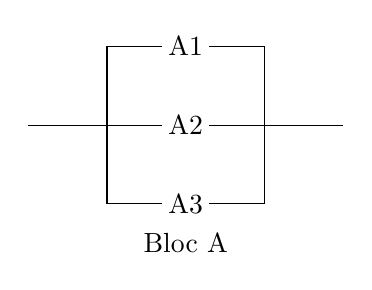
\begin{tikzpicture}	
		
		\draw (0,0)--(1,0);
            \draw (3,0)--(4,0);

            
		\node at (2,1) {A1};
		\node at (2,0) {A2};
            \node at (2,-1) {A3};
            
            
            \draw (1,1) -- (1.7,1); 
            \draw (1,0) -- (1.7,0); 
            \draw (1,-1) -- (1.7,-1); 
            
            
            \draw (2.3,1) -- (3,1); 
            \draw (2.3,0) -- (3,0); 
            \draw (2.3,-1) -- (3,-1); 

            
            \draw (1,0) -- (1,1); 
            \draw (1,0) -- (1,-1); 

            
            \draw (3,0) -- (3,1); 
            \draw (3,0) -- (3,-1); 
		
		\node at (2,-1.5) {Bloc A};
    \end{tikzpicture} \end{center}
\end{figure}
	
 Le bloc A contient trois éléments. Nous avons que
\begin{itemize}
    \item L'élément A1 fonctionne avec une probabilité de 0,60.
    \item L'élément A2 fonctionne avec une probabilité de 0,50.
    \item L'élément A3 fonctionne avec une probabilité de 0,60.
\end{itemize}
Pour que le montage fonctionne, au moins un élément du bloc A doit fonctionner. Les éléments d'un bloc fonctionnent de façon indépendante.
	

 Quelle est la probabilité que le montage ne fonctionne pas? 

 \begin{oneparcheckboxes}
		\choice 0,08
		\correctchoice 0,92
		\choice 0,18 
		\choice 0,82
		\choice 0,63
\end{oneparcheckboxes}

\begin{solution}
On cherche la loi de
		\begin{eqnarray*}
			{X}_2|{X}_1=101 &\sim& N\left(\mu_2 +\rho\, \sigma_2\, \left(\frac{x_1-\mu_1}{\sigma_1}\right),\sigma_2^2 \,\left(1-\rho_2^2\right)\right)\\
			&\sim& N\left(84 +0.8\times 5\times \left(\frac{101-92}{3}\right),25 \,\left(1-0.8^2\right)\right)\\
			&\sim& N\left(96, 9 \right)
	\end{eqnarray*}
\end{solution}

.
\end{A23}

\begin{A23}
\question (A23)  Une personne a $n$ clés sur son porte-clés.
Parmi ces $n$ clés, $k$ clés déverrouillent une même serrure. 
La personne tente de déverrouiller cette serrure en utilisant une succession de clés, avec remise, c'est-à-dire qu'après avoir tenté avec une clé qui ne fonctionne pas, la clé est remise dans le lot.
On note $X$ la variable aléatoire du nombre de clés testées avant que la serrure soit déverrouillée.
Que vaut $P(X=k)$?

\begin{oneparcheckboxes}
    \choice $\displaystyle \left(\frac{n-k}{n}\right)^{k-1}\frac{k}{n}$
    \choice $\displaystyle \binom{n}{k}\left(\frac{k}{n}\right)^{k}\left(1-\frac{k}{n}\right)^{n-k}$
    \correctchoice $\displaystyle \binom{k-1}{n-1}\left(\frac{k}{n}\right)^{n}\left(1-\frac{k}{n}\right)^{n-k}$
    \choice $\displaystyle \frac{k}{n}$
\end{oneparcheckboxes}
\end{A23}

\begin{A23}
\question (A23) \label{A23-I5-pa} Soient $A$, $B$ et $C$ trois événements avec $P(A)=0,5$, $P(B)=0,5$, $P(C)=0,2$, $P(A\cap B)=0,25$. Nous avons aussi que $C$ est indépendant de l'événement $A$ et de l'événement $B$. Dites si chacun des énoncés ci-dessous est vrai ou faux. Votre réponse doit être justifiée en mots ou par des calculs. Un vrai ou faux sans justification n'aura aucun point.

\begin{parts}

\part[3] Les événements $A$ et $B$ sont indépendants.

     \begin{oneparcheckboxes}
		\choice VRAI
		\correctchoice FAUX
\end{oneparcheckboxes}\\
{\bf Justification:}

\part[3] $P(A\cup C)= 0,6$.

\begin{oneparcheckboxes}
		\choice VRAI
		\correctchoice FAUX
\end{oneparcheckboxes}\\
{\bf Justification:}

\part[3] Les événements $A$ et $B$ forment une partition de l'espace échantillonnal.

     \begin{oneparcheckboxes}
		\choice VRAI
		\correctchoice FAUX
\end{oneparcheckboxes}\\
{\bf Justification:}
\end{parts}

 .
\end{A23}

\begin{A24}
\question (A24) \label{A24-I1-module1_1} \textit{Les questions (a) et (b) sont indépendantes.}
\begin{parts}
\part On nous donne les probabilités suivantes:
\[
\begin{aligned}
    & P(A) = 0,45 \\
    & P(B) = 0,55 \\
    & P(C) = 0,1 \\
    & P(A\cap C) = 0 \\
    & P(B\cap C) = 0 \\
    & P(A | B) = 0,20 \\
    & 
\end{aligned}
\]
\begin{subparts}
\subpart[3] Lequel des énoncés suivants est vrai?
\begin{checkboxes}

\choice $P(A \cup B) = 1$
\choice $A$, $B$ et $C$ sont mutuellement exclusifs.
\correctchoice $A$ et $C$ sont indépendants.
\choice Comme $P(A)+P(B)=1$, l'intersection de $A$ et $B$ doit être vide, c'est-à-dire $A\cap B = \emptyset$.
\choice $A$ et $C$ sont mutuellement exclusifs. 
\choice Aucun des énoncés précédents n'est vrai.

\end{checkboxes}

\subpart[4] \(A\) et \(B\) sont indépendants.

     \begin{oneparcheckboxes}
		\choice VRAI
		\correctchoice FAUX
\end{oneparcheckboxes}\\
{\bf Justification:}

\end{subparts}
 
 
\part[3] Un certain item manufacturé est visuellement vérifié par deux inspecteurs à la suite. 
Le premier inspecteur détecte 90\% des items défectueux. 
Parmi les item défectueux qui passent le premier inspecteur sans être détectés, 60\% ne seront pas détectés par le deuxième inspecteur.
Quelle est la probabilité qu'un item défectueux ne soit repéré par aucun inspecteur?

\begin{checkboxes}
    \choice $90\%$
    \choice $60\%$
    \choice $10\%$
    \choice $40\%$
    \choice $54\%$
    \choice $6\%$
    \choice $9\%$
    \choice $4\%$
    \choice $36\%$
    \choice $24\%$
    
\end{checkboxes}
\end{parts}
\end{A24}

\begin{A24}
\question (A24) Une compagnie d’assurances subdivise ses clients en assurance automobile en trois catégories : les jeunes (16 à 29 ans), les personnes d’âges moyen (30 à 59 ans) et les personnes âgées (60 ans et plus). Selon l’expérience de la compagnie, la probabilité qu’un jeune soit impliqué dans un accident pendant l’année est de 0.12, celle d’une personne d’âge moyen, de 0.06 et celle d’une personne âgée, de 0.10. La clientèle de la compagnie est formée de 30\% de jeunes, de 45\% de personnes d’âge moyen et de 25\% de personnes âgées. 

\begin{parts}
\part[5]  Si on choisit un client de cette compagnie au hasard, quelle est la probabilité que ce client ait un accident pendant l’année?	

\begin{solution}
    Désignons les événements suivants par :

    J=''Le client choisi est jeune''

    M=''Le client choisi est d'âge moyen''

    A=''Le client choisi est âgé'

    I=''Le client est impliqué dans un accident pendant l'année''

    En utilisant la formule des probabilités totale, on obtient 
    $$
    \begin{array}{ccl}
       P(I)  &=& P(J)P(I|J) + P(M)P(I|M)+P(A)P(I|A)\\  \\
         &= & 0.30x0.12+0.45x0.06+0.25x0.10\\  \\
          &=&0.0880
    \end{array}
   $$

\end{solution}

\part[5]  Si on constate que le client choisi au hasard a eu un accident cette année, quelle est la probabilité que ce soit un jeune?                        
\begin{solution}
    Selon la formule de Bayes, on a:
 $$
    \begin{array}{ccl}
       P(J|I)  &=& \frac{P(J)P(I|J)}{P(J)P(I|J) + P(M)P(I|M)+P(A)P(I|A)}\\  \\
         &= & \frac{0.30x0.12}{0.45x0.06+0.25x0.10}\\ \\
          &=&0.4091
    \end{array}
   $$  
    
\end{solution}
\end{parts}
\end{A24}

\begin{A24}
\question (A24) Une urne contient 25 balles.
 Parmi ces balles, 5 sont rouges, 5 sont vertes, 5 sont bleues, 5 sont jaunes et 5 sont noires.
 Pour chacune des couleurs, les balles sont numérotées de 1 à 5.

 \begin{parts}
     \part[2] Combien existe-t-il de sous-ensembles contenant 5 balles?
    \begin{solution}
        On parle de sous-ensembles, donc l'ordre n'est pas important. Il s'agit donc d'une combinaison:
        $$C_5^{25}=53130$$
    \end{solution}
     

    \part[2] Combien existe-t-il de sous-ensembles contenant 5 balles, dont au moins une noire?
        \begin{solution}
        Ici on peut simplement dire qu'il s'agit du nombre de sous-ensembles total moins ceux qui ne contiennent aucune balle noire.

        $$C_5^{25}-C_{5}^{20}=37626$$

        

    \end{solution}
     
     \part[3] Combien existe-t-il de sous-ensembles contenant 5 balles et exactement 2 balles jaunes?
            \begin{solution}
  On peut séparer en deux événements: piger 3 balles parmi les 20 et 2 balles parmi les jaunes:

  $$C_{3}^{20}\times C_{2}^5=11400$$

        

    \end{solution}   

 \end{parts}
\end{A24}

\begin{H25}
\question (H25) La tuberculose bovine est une maladie très contagieuse. Cette maladie est apparue dans  le cheptel bovin d'un pays et touche $10 \%$ de ce cheptel. Des études statistiques ont montré que la probabilité pour un animal d'avoir un test positif à cette maladie sachant qu'il est malade est de $95 \%$  et que celle d'avoir un test négatif sachant qu'il n'est pas atteint par la maladie est de $90 \%$ . Définissons les événements suivants :\\
\begin{tabular}{ l}
$T$ : avoir un test positif à cette maladie pour un bovin choisi au hasard parmi le cheptel.\\
$M$ : être malade pour un bovin choisi au hasard parmi le cheptel.
\end{tabular}

\medskip
\begin{parts}
\part [4] Déterminez la probabilité d'avoir un test positif à cette maladie pour un bovin choisi au hasard parmi le cheptel sachant que celui-ci n'est pas malade.

\part [4] Calculez la probabilité pour un bovin choisi au hasard parmi le cheptel d'avoir un test positif à cette maladie.

\part [4] Calculez la probabilité qu'un bovin choisi au hasard parmi le cheptel soit malade sachant que le test est positif.
\end{parts}
\end{H25}

\begin{H25}
\question (H25) Soit $A$, $B$ et $C$ trois événements avec $P(A)=0,5$, $P(B)=0,5$, $P(C)=0,2$, $P(A\cap B)=0,25$. Nous avons aussi que $C$ est indépendant de l'événement $A$ et de l'événement $B$. Dites si chacun des énoncés ci-dessous est vrai ou faux. Votre réponse doit être justifiée en mots ou par des calculs. Un vrai ou faux sans justification n'aura aucun point.

\begin{parts}

\part[3] Les événements $A$ et $B$ sont indépendants.

     \begin{oneparcheckboxes}
		\correctchoice VRAI
		\choice FAUX
\end{oneparcheckboxes}\\
{\bf Justification:}
\begin{solution}
    Comme $P(A)P(B)=0,5 \times 0,5 = 0,25 = P(A\cap B)$, les événements sont indépendants.
\end{solution}

\part[3] $P(A\cup C)= 0,6$.

\begin{oneparcheckboxes}
		\correctchoice VRAI
		\choice FAUX
\end{oneparcheckboxes}\\
{\bf Justification:}
\begin{solution}
    Comme $A$ et $C$ sont indépendants, $P(A\cap C) = 0,5 \times 0,2 =0.1$.

    Donc $P(A \cup C)=P(A)+P(C)-P(A\cap C)=0,5+0,2-0,1=0,6$
\end{solution}

\part[3] Les événements $A$ et $B$ forment une partition de l'espace échantillonnal.

     \begin{oneparcheckboxes}
		\choice VRAI
		\correctchoice FAUX
\end{oneparcheckboxes}\\
{\bf Justification:}
\begin{solution}
    Pour qu'ils forment une partition de $\mathcal{U}$, ils doivent être mutuellement exclusifs, i.e. $A\cap B= \emptyset$, ce qui devrait donner $P(A\cap B)=0$, ce qui n'est pas le cas.
\end{solution}
\end{parts}
\end{H25}

\begin{H25}
\question (H25) Après un certain nombre de tours pendant une partie de \textit{Scrabble}, les 15 lettres suivantes n'ont toujours pas été choisies et sont donc encore dans le sac:
$$\{a, e, i, g, h, l, n, o, p, t, t, v, v, w, x\}.$$

\begin{parts}
    \part[4] Si Alex doit piger 4 lettres au hasard dans le sac, quelle est la probabilité que ces lettres soit les lettres de son prénom, dans le bon ordre? Laissez des traces de votre démarche.
\begin{solution}
    Soit l'événement $A:$ Alex pige les lettres de son nom dans l'ordre.
    
    Comme l'ordre est important, la probabilité est

    \begin{align*}
        P(A)&=\frac{1}{15}\times\frac{1}{14}\times\frac{1}{13}\times\frac{1}{12}\\
        P(A)&= \frac{1}{32760}
    \end{align*}
\end{solution}

     
    \part[6] Supposons qu'Alex a pigé $\{i, g, t, w\}$. Il reste donc 
$\{a, e, h, l, n, o, p, t, v, v, x\}$ dans le sac. C'est maintenant au tour d'Eva de piger 4 lettres. Quelle est la probabilité que parmi les 4 lettres qu'elle doit piger, elle pige les lettres qui forment son prénom (peu importe l'ordre)? Laissez des traces de votre démarche.
\begin{solution}
     Soit l'événement $E:$ Eva pige au moins les 3 lettres de son nom peu importe l'ordre.
    
    Comme l'ordre n'est pas important.

    \begin{align*}
        P(E)&= \frac{\binom{1}{1}\binom{1}{1}\binom{2}{1}\binom{8}{1}}{\binom{11}{4}}\\
        &= \frac{16}{330}\\
        &\approx 0,0485
    \end{align*}
\end{solution}
\end{parts}
\end{H25}

\begin{A25}
\question (A25) 
Une entreprise de tourisme aérien propose des tours en hélicoptère. Elle dispose de 4 hélicoptères, de 4 pilotes et de 8 hôtesses de l’air. Chaque hélicoptère doit être opéré par 1 pilote et accompagné de 2 hôtesses de l’air pour assurer le confort et la sécurité des passagers.

De combien de façons différentes l’entreprise peut-elle attribuer les pilotes et les hôtesses aux hélicoptères ?

\begin{solution}
Le nombre total de choix correspond exactement au nombre total de façons d’attribuer pilotes et hôtesses:
\\
\begin{itemize}
    \item Attribution des pilotes : $4!=24$ façons
    \item Attribution des hôtesses : 
\begin{align*}
  \binom{8}{2} \times \binom{6}{2} \times \binom{4}{2} \times \binom{2}{2} 
= 28 \times 15 \times 6 \times 1 = 2520  \text{ façons}. 
\end{align*}
\end{itemize}
Donc le nombre total de choix : $24 \times 2520=60480$. Donc il y a 60480 façons différentes d’attribuer les pilotes et les hôtesses aux hélicoptères.
\end{solution}
\end{A25}

\begin{A25}
\question (A25)  
\begin{center}
    

\begin{tikzpicture}[scale=1.1]

\coordinate (A) at (-1,2.2);

\coordinate (B) at (-5,0.0);
\coordinate (C) at (-1.9,0.6);
\coordinate (D) at (1.8,0.6);
\coordinate (E) at (6.1,0.9);

\coordinate (F) at (-6,-1);
\coordinate (G) at (-5,-1.1);
\coordinate (H) at (-4,-1);

\coordinate (I) at (0,-2.1);

\coordinate (J) at (3.3,-1.4);

\coordinate (K) at (5.1,-1.4);
\coordinate (L) at (6.1,-1.4);
\coordinate (M) at (7.1,-1.4);

\node[pt,above] at (A) {A};
\node[pt,left]  at (B) {B};

\node[pt,above] at (C) {C};
\node[pt,above] at (D) {D};
\node[pt,above right] at (E) {E};

\node[pt,below] at (F) {F};
\node[pt,below] at (G) {G};
\node[pt,below] at (H) {H};

\node[pt,below] at (I) {I};
\node[pt,above left] at (J) {J};
\node[pt,below] at (K) {K};
\node[pt,below] at (L) {L};
\node[pt,below] at (M) {M};

\draw[mid arrow] (A) -- (B);
\draw[mid arrow] (A) -- (C);
\draw[mid arrow] (A) -- (D);
\draw[mid arrow] (A) -- (E);

\draw[mid arrow] (B) -- (F);
\draw[mid arrow] (B) -- (G);
\draw[mid arrow] (B) -- (H);

\draw[mid arrow] (B) -- (I);

\draw[mid arrow] (C) -- (I);

\draw[mid arrow] (D) -- (I);

\draw[mid arrow] (E) -- (I);
\draw[mid arrow] (E) -- (J);
\draw[mid arrow] (E) -- (K);
\draw[mid arrow] (E) -- (L);
\draw[mid arrow] (E) -- (M);

\draw[mid arrow] (J) -- (I);

\node[dot] at (A) {};
\node[dot] at (B) {};
\node[dot] at (C) {};
\node[dot] at (D) {};
\node[dot] at (E) {};
\node[dot] at (F) {};
\node[dot] at (G) {};
\node[dot] at (H) {};
\node[dot] at (I) {};
\node[dot] at (J) {};
\node[dot] at (K) {};
\node[dot] at (L) {};
\node[dot] at (M) {};

\end{tikzpicture}
\end{center}

Une randonneuse part du point A en choisissant au hasard parmi les sentiers $AB$, $AC$, $AD$ et $AE$.
Elle s'arrête seulement lorsqu'elle est arrivée à $F,G,H,I,K,L$ ou $M$.
Quelle est la probabilité qu'elle ne s'arrête pas au point $M$?

\begin{checkboxes}
    \choice 1/7
    \choice 1/8
    \choice 1/5
    \choice 1/20
    \choice 1/24
    \choice 1/16
    \choice 6/7
    \choice 7/8
    \choice 4/5
    \correctchoice 19/20
    \choice 23/24
    \choice 15/16
    \choice 10/11
\end{checkboxes}
\end{A25}

\begin{A25}
\question (A25) \label{A25-I19-module1_1}  
On nous donne les probabilités suivantes:
\[
\begin{aligned}
    & P(A) = 0,45 \\
    & P(B) = 0,25 \\
    & P(C) = 0,30 \\
    & P(C|A) = 0,30 \\
    & P(C|B) = 0,30 \\
    & P(A \cap B) = 0,05 \\
\end{aligned}
\]

Cochez tous les énoncés qui sont \textbf{vrais}, sachant que deux énoncés sont vrais. \textit{Chaque énoncé qui est coché alors qu'il ne devrait pas l'être annule les points d'un élément coché qui devrait l'être.}
\begin{checkboxes}
\choice $P(A \cup B) = 0,70$
\correctchoice $ P(A \cap \overline{B}) = 0,40 $
\choice $ P(A \cap C) = 0,1575 $
\choice $ P(A \cup C) = 0,75 $
\choice $A$ et $B$ sont indépendants
\correctchoice $A$ et $C$ sont indépendants
\choice Comme $B$ et $C$ sont indépendants, ils sont mutuellement exclusifs
\end{checkboxes}
\end{A25}

\begin{A25}
\question (A25)  Soit $A$ et $B$, deux événements de $\mathcal{U}$, avec $P(A)>0$ et $P(B)>0$.Quel énoncé est \textbf{toujours} vrai?

\begin{checkboxes}
    \choice Si $P(A)+P(B)=1$, $A$ et $B$ forment une partition de $\mathcal{U}$.
    \choice Si $P(A\cap B)=0$, $A$ et $B$ sont indépendants.
    \correctchoice Si $A$ et $B$ sont indépendants, ils ne sont pas mutuellement exclusifs.
    \choice Si $A\subset B$, le fait que $B$ se réalise implique que $A$ se réalise.
\end{checkboxes}
\end{A25}

\begin{A25}
\question (A25) Supposons que dans la population, il y a $51\%$ d'hommes ($H$) et $49\%$ de femmes ($F$), et que le daltonisme ($D$) est réparti de cette façon:

\begin{table}[h]
    \centering
    \begin{tabular}{l|c|c}
    \hline \hline
        & Hommes ($H$) & Femmes ($F$) \\
    \hline
        Daltoniens ($D$) & 0,04 & $XXX$ \\ 
        Non daltoniens ($\overline{D}$) &0,47 & $YYY$ \\
        \hline

        \hline
    \end{tabular}
\end{table}

Nous savons que la probabilité qu'une femme choisie au hasard soit daltonienne est de $\frac{1}{245}$.

\begin{parts}
    \part[6]Quelle est la probabilité qu'une personne choisie au hasard soit une femme et soit non daltonienne?
\begin{solution}
    Nous savons que $P(D|F)=\frac{1}{245}$. Nous avons donc 
    \begin{align*}
        P(D|F)&= \frac{P(D\cap F)}{P(F)}\\
        \frac{1}{245}&= \frac{P(D\cap F)}{0,49}\\
        0,49 *\frac{1}{245}&=P(D\cap F)\\
        P(D\cap F)&=\frac{1}{500}
    \end{align*}
    Nous savons donc que $XXX=\frac{1}{500}$. Comme nous avons que $0,04+0,47+XXX+YYY=1$, nous déduisons $YYY=0,488$
\end{solution}
    
    \part[3] $H$ et $F$ sont indépendants.

     \begin{oneparcheckboxes}
		\choice VRAI
		\correctchoice FAUX
\end{oneparcheckboxes}\\
{\bf Justification:}

        \part[3] $H$ et $D$ sont indépendants.

     \begin{oneparcheckboxes}
		\choice VRAI
		\correctchoice FAUX
\end{oneparcheckboxes}\\
{\bf Justification:}
\end{parts}
\end{A25}

\begin{A25}
\question (A25)  Considérons le montage électronique représenté ci-dessous.
	
\begin{figure}[h!]
    
    \begin{center}	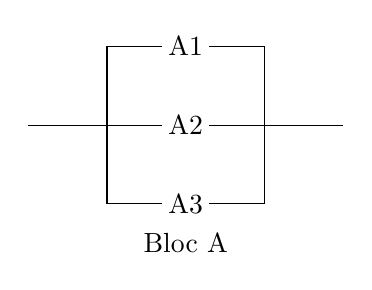
\begin{tikzpicture}	
		
		\draw (0,0)--(1,0);
            \draw (3,0)--(4,0);

            
		\node at (2,1) {A1};
		\node at (2,0) {A2};
            \node at (2,-1) {A3};
            
            
            \draw (1,1) -- (1.7,1); 
            \draw (1,0) -- (1.7,0); 
            \draw (1,-1) -- (1.7,-1); 
            
            
            \draw (2.3,1) -- (3,1); 
            \draw (2.3,0) -- (3,0); 
            \draw (2.3,-1) -- (3,-1); 

            
            \draw (1,0) -- (1,1); 
            \draw (1,0) -- (1,-1); 

            
            \draw (3,0) -- (3,1); 
            \draw (3,0) -- (3,-1); 
		
		\node at (2,-1.5) {Bloc A};
    \end{tikzpicture} \end{center}
\end{figure}
	
 Le bloc A contient trois éléments. Nous avons que
\begin{itemize}
    \item L'élément A1 fonctionne avec une probabilité de 0,60.
    \item L'élément A2 fonctionne avec une probabilité de 0,50.
    \item L'élément A3 fonctionne avec une probabilité de 0,60.
\end{itemize}
Pour que le montage fonctionne, au moins un élément du bloc A doit fonctionner. Les éléments d'un bloc fonctionnent de façon indépendante.
	

 Quelle est la probabilité que le montage ne fonctionne pas? 

 \begin{oneparcheckboxes}
		\choice 0,08
		\correctchoice 0,92
		\choice 0,18 
		\choice 0,82
		\choice 0,63
\end{oneparcheckboxes}
\end{A25}

\begin{H26}
\question (H26) 

On considère l’espace échantillonnal
\[
U = \{a,b,c,d,e,f\}
\]
et les ensembles
\[
A = \{a,b,c\}, \qquad
B = \{b,d,e\}, \qquad
C = \{c,e,f\}.
\]

Calculez les ensembles suivants :\\
\begin{parts}
\part[3]\(A \cup B^c\)
\begin{solution}
On a 
$B^c = \Omega \setminus B = \{a,c,f\}.$
Donc, \[
A \cup B^c = \{a,b,c\} \cup \{a,c,f\} = \{a,b,c,f\}.
\]
\end{solution}

\part[3] \((A \cup B) \cap C\)   
\begin{solution}
\[
A \cup B = \{a,b,c,d,e\}
\]
\[(A \cup B) \cap C = \{a,b,c,d,e\} \cap \{c,e,f\} = \{c,e\}.
\]
\end{solution}

\end{parts}
\end{H26}

\begin{H26}
\question (H26) 

Une station de radio possède une banque de \(14\) chansons.
\begin{itemize}
\item \(4\) chansons sont du même artiste (artiste A);
\item les \(10\) autres chansons sont toutes d’artistes différents, et différents de A.
\end{itemize}

On choisit au hasard \(5\) chansons distinctes pour une liste de lecture. Quelle est la probabilité que la liste contienne \emph{exactement deux} chansons de l’artiste A?

\begin{solution}
Le nombre total de choix possibles de \(5\) chansons parmi \(14\) est
\[
\binom{14}{5}.
\]

Pour avoir exactement deux chansons de l’artiste A :
\begin{itemize}
\item on choisit \(2\) chansons parmi les \(4\) de l’artiste A : \(\binom{4}{2}\);
\item on choisit \(3\) chansons parmi les \(10\) autres : \(\binom{10}{3}\).
\end{itemize}

Le nombre de choix favorables est donc
\[
\binom{4}{2}\binom{10}{3}.
\]

La probabilité demandée vaut
\[
\mathbb{P}(\text{exactement 2 de A})
=
\frac{\binom{4}{2}\binom{10}{3}}{\binom{14}{5}}.
\]

On peut simplifier numériquement :
\[
\binom{4}{2}=6,\qquad \binom{10}{3}=120,\qquad \binom{14}{5}=2002,
\]
donc
\[
\mathbb{P}=\frac{6\cdot 120}{2002}=\frac{720}{2002}=\frac{360}{1001}.
\]

\[
\boxed{\mathbb{P}=\frac{360}{1001}.}
\]
\end{solution}
\end{H26}

\begin{H26}
\question (H26) 

Un sac contient 40 billes rouges, 40 billes vertes et 20 billes bleues.
Sur certaines de ces billes, une étoile a été dessinée.
Nous savons que la probabilité de choisir une bille sans étoile parmi les billes rouges est de $0,875$, la probabilité de choisir une bille qui est verte et qui a une étoile est de $0,1$ et la probabilité de choisir une bille qui a une étoile parmi les billes bleues est de $0,5$.

En utilisant les événements suivants:

\begin{itemize}
    \item R: la bille est rouge
    \item V: la bille est verte
    \item B: la bille est bleue
    \item E: une étoile est dessinée sur la bille
\end{itemize}

\begin{parts}
    \part[3] Tracez le diagramme de Venn qui représente cette situation. \textit{Vous n'avez qu'à identifier les événements et \textbf{l'espace échantillonnal}. Il n'est pas nécessaire d'inscrire les probabilités.}
\begin{solution}

    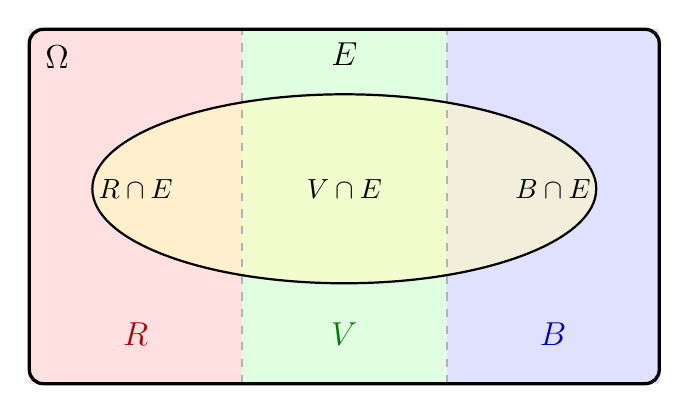
\begin{tikzpicture}[font=\small]

\def\W{8}    
\def\H{4.5}  
\def\xR{2.7} 
\def\xV{5.3} 

\fill[red!12]   (0,0) rectangle (\xR,\H);
\fill[green!12] (\xR,0) rectangle (\xV,\H);
\fill[blue!12]  (\xV,0) rectangle (\W,\H);

\fill[yellow!25, opacity=0.55]
    (0.5*\W, 0.55*\H) ellipse [x radius=3.2, y radius=1.2];

\draw[thick, dashed, gray!60] (\xR,0) -- (\xR,\H);
\draw[thick, dashed, gray!60] (\xV,0) -- (\xV,\H);

\draw[thick] (0.5*\W, 0.55*\H) ellipse [x radius=3.2, y radius=1.2];

\draw[very thick, rounded corners=5pt] (0,0) rectangle (\W,\H);

\node[font=\normalsize] at (0.5*\xR, 0.55*\H)         {$R\cap E$};
\node[font=\normalsize] at (0.5*\xR+0.5*\xV, 0.55*\H) {$V\cap E$};
\node[font=\normalsize] at (0.5*\xV+0.5*\W, 0.55*\H)  {$B\cap E$};

\node[font=\large, red!70!black]   at (0.5*\xR, 0.14*\H)         {$R$};
\node[font=\large, green!50!black] at (0.5*\xR+0.5*\xV, 0.14*\H) {$V$};
\node[font=\large, blue!70!black]  at (0.5*\xV+0.5*\W, 0.14*\H)  {$B$};

\node[font=\large] at (0.5*\W, 0.93*\H) {$E$};

\node[anchor=north west, font=\large] at (0.08,\H-0.08) {$\Omega$};

\end{tikzpicture}
\end{solution}
    

    \part[8] Si vous avez pigé une bille avec une étoile, quelle est la probabilité que celle-ci soit bleue?

    \begin{solution}
        On cherche $P(B|E)$

        \begin{align*}
            P(B|E)&=\frac{P(B\cap E)}{P(E)}\\
            &=\frac{P(E|B)P(B)}{P(E\cap R)+P(E\cap V)+P(E\cap B)}\\
            &=\frac{P(E|B)P(B)}{P(E|R)P(R)+P(E|V)P(V)+P(E|B)P(B)}\\
            &=\frac{0,5\times 0,2}{(1-0,875)\times 0,4+0,1+0,5\times 0,2}\\
            &=\frac{2}{5}
        \end{align*}
    \end{solution}

\part  \begin{subparts}
        \subpart[1] Les événements R et V sont indépendants.
        
        \begin{oneparcheckboxes}
            \choice Vrai
            \correctchoice Faux
        \end{oneparcheckboxes}

        \subpart[1] Les événements R et E sont indépendants.
        
        \begin{oneparcheckboxes}
            \choice Vrai
            \correctchoice Faux
        \end{oneparcheckboxes}

        \subpart[1] Les événements R, V et B forment une partition de l'espace échantillonnal.
        
        \begin{oneparcheckboxes}
            \correctchoice Vrai
            \choice Faux
        \end{oneparcheckboxes}
    \end{subparts}
    
\end{parts}
\end{H26}

\begin{H26}
\question (H26) 
Soit deux événements $A$ et $B$ formant une partition de l'espace échantillonnal, avec $P(A)=0,7$. \\On a aussi que $P(D\mid A)=0,02$, $P(D\mid B)=0,05$.

Quelle expression permet de calculer $P(B\mid D)$ ?\\

\begin{checkboxes}
\choice $\dfrac{0,3\times 0,05}{0,02 + 0,05}$\\[4pt]
\choice $\dfrac{0,05}{0,7\times 0,02 + 0,3\times 0,05}$\\[4pt]
\choice $\dfrac{0,7\times 0,02}{0,7\times 0,02 + 0,3\times 0,05}$\\[4pt]
\correctchoice $\dfrac{0,3\times 0,05}{0,7\times 0,02 + 0,3\times 0,05}$\\[4pt]
\choice $\dfrac{0,3\times 0,05}{0,7\times 0,02 + 0,7\times 0,05}$
\end{checkboxes}
\end{H26}

\begin{H26r}
\question (H26r)  

On sait que \(P(A)=0{,}3\), \(P(B)=0{,}2\) et \(P(A^c \cap B)=0{,}1\).
Calculez \(P(A \cap B)\).

\begin{solution}
On décompose l’événement \(B\) :
\[
B = (A \cap B) \cup (A^c \cap B),
\]
où les deux événements sont disjoints. Par additivité des probabilités,
\[
P(B) = P(A \cap B) + P(A^c \cap B).
\]

On isole alors \(P(A \cap B)\) :
\[
P(A \cap B) = P(B) - P(A^c \cap B) = 0{,}2 - 0{,}1 = 0{,}1.
\]

\[
\boxed{P(A \cap B) = 0{,}1}
\]    
\end{solution}
\end{H26r}

\begin{H26r}
\question (H26r) 

Douze personnes participent à une soirée micro-ouvert, dont Julie. Un programme de la soirée consiste à choisir \(5\) personnes parmi les \(12\) et à fixer un ordre de passage pour ces \(5\) personnes. Une contrainte est imposée :
\emph{la première personne à passer doit être l’une des trois personnes désignées comme animateurs}.
Julie n’est \emph{pas} animatrice.

Si on choisit un programme au hasard parmi tous les programmes respectant cette contrainte, quelle est la probabilité que Julie soit choisie et qu’elle passe en troisième position?

\begin{solution}

\textbf{Nombre total de programmes possibles}

On choisit d’abord l’animateur qui passe en premier : \(3\) choix.

Puis on choisit et ordonne \(4\) autres personnes parmi les \(11\) restantes :
\[
{}_{11}P_{4}.
\]

Le nombre total de programmes est donc
\[
3\times {}_{11}P_{4}
=3\times \frac{11!}{7!}.
\]

\medskip
\textbf{Cas favorables}

On impose que Julie soit choisie et qu’elle passe en troisième position.

\emph{Étape 1 :} choisir l’animateur en première position : \(3\) choix.

\emph{Étape 2 :} choisir les \(3\) autres personnes parmi les \(10\) restantes (en excluant Julie et l’animateur choisi) :
\[
\binom{10}{3}.
\]

\emph{Étape 3 :} ordonner ces \(3\) personnes et Julie dans les positions
\(2,3,4,5\), en imposant que Julie soit en position \(3\).

Il reste alors \(3!\) ordres possibles.

Le nombre de programmes favorables est donc
\[
3\times \binom{10}{3}\times 3!
\]

\medskip
\textbf{Probabilité}

\[
\mathbb{P}(\text{Julie choisie et en 3e})
=
\frac{3\,\binom{10}{3}\,3!}{3\,{}_{11}P_{4}}
=
\frac{\binom{10}{3}\,3!}{{}_{11}P_{4}}.
\]

On simplifie :
\[
\binom{10}{3}\,3!
=
\frac{10!}{7!},
\qquad
{}_{11}P_{4}=\frac{11!}{7!}.
\]

Donc
\[
\mathbb{P}(\text{Julie choisie et en 3e})
=
\frac{10!}{11!}
=
\frac{1}{11}.
\]

\[
\boxed{\mathbb{P}=\frac{1}{11}.}
\]
\end{solution}
\end{H26r}

\begin{H26r}
\question (H26r) 

Un magasin de jouets vend 3 types de figurines: des dragons, des licornes et des phénix. Parmi les figurines vendues, $50\%$ sont des dragons, $30\%$ sont des licornes et $20\%$ sont des phénix. Certaines figurines sont défectueuses. On sait que $10\%$ des dragons sont défectueux, la probabilité de choisir une figurine qui est une licorne et qui est défectueuse est de $0{,}06$, et $25\%$ des phénix sont défectueux.

En utilisant les événements suivants:
\begin{itemize}
    \item D: la figurine est un dragon
    \item L: la figurine est une licorne
    \item P: la figurine est un phénix
    \item F: la figurine est défectueuse
\end{itemize}

\begin{parts}
    \part[2] Tracez le diagramme de Venn qui représente cette situation. \textit{Vous n'avez qu'à identifier les événements et \textbf{l'espace échantillonnal}. Il n'est pas nécessaire d'inscrire les probabilités.}

\begin{solution}
    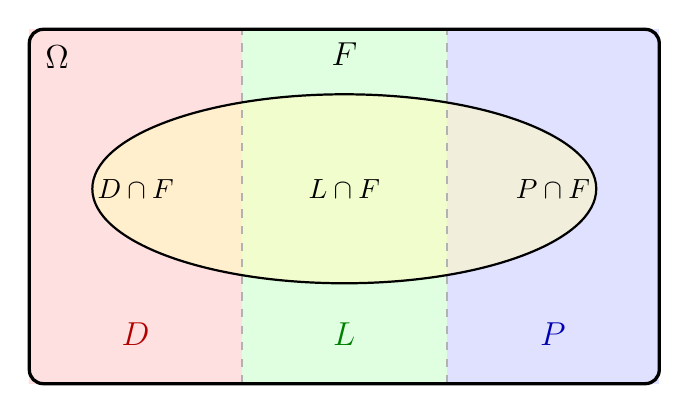
\begin{tikzpicture}[font=\small]

\def\W{8}    
\def\H{4.5}  
\def\xD{2.7} 
\def\xL{5.3} 

\fill[red!12]    (0,0) rectangle (\xD,\H);
\fill[green!12]  (\xD,0) rectangle (\xL,\H);
\fill[blue!12]   (\xL,0) rectangle (\W,\H);

\fill[yellow!25, opacity=0.55]
    (0.5*\W, 0.55*\H) ellipse [x radius=3.2, y radius=1.2];

\draw[thick, dashed, gray!60] (\xD,0) -- (\xD,\H);
\draw[thick, dashed, gray!60] (\xL,0) -- (\xL,\H);

\draw[thick] (0.5*\W, 0.55*\H) ellipse [x radius=3.2, y radius=1.2];

\draw[very thick, rounded corners=5pt] (0,0) rectangle (\W,\H);

\node[font=\normalsize] at (0.5*\xD, 0.55*\H)         {$D\cap F$};
\node[font=\normalsize] at (0.5*\xD+0.5*\xL, 0.55*\H) {$L\cap F$};
\node[font=\normalsize] at (0.5*\xL+0.5*\W, 0.55*\H)  {$P\cap F$};

\node[font=\large, red!70!black]   at (0.5*\xD, 0.14*\H)         {$D$};
\node[font=\large, green!50!black] at (0.5*\xD+0.5*\xL, 0.14*\H) {$L$};
\node[font=\large, blue!70!black]  at (0.5*\xL+0.5*\W, 0.14*\H)  {$P$};

\node[font=\large] at (0.5*\W, 0.93*\H) {$F$};

\node[anchor=north west, font=\large] at (0.08,\H-0.08) {$\Omega$};
\end{tikzpicture}
\end{solution}
    

    \part[5] Si vous avez acheté une figurine défectueuse, quelle est la probabilité que ce soit un phénix?

    \begin{solution}
        On connaît: $P(D)=0{,}5$, $P(L)=0{,}3$, $P(P)=0{,}2$, $P(F|D)=0{,}1$, $P(L\cap F)=0{,}06$ (donc $P(F|L)=\frac{0{,}06}{0{,}3}=0{,}2$), $P(F|P)=0{,}25$.

        On cherche $P(P|F)$.

        \begin{align*}
            P(F)&=P(F|D)\,P(D)+P(F|L)\,P(L)+P(F|P)\,P(P)\\
            &=0{,}1\times 0{,}5+0{,}2\times 0{,}3+0{,}25\times 0{,}2\\
            &=0{,}05+0{,}06+0{,}05=0{,}16
        \end{align*}

        Donc
        \begin{align*}
            P(P|F)&=\frac{P(F|P)\,P(P)}{P(F)}
            =\frac{0{,}25\times 0{,}2}{0{,}16}
            =\frac{0{,}05}{0{,}16}
            =\frac{5}{16}
        \end{align*}
    \end{solution}

\part  \begin{subparts}
        \subpart[1] Les événements D et L sont indépendants.
        
        \begin{oneparcheckboxes}
            \choice Vrai
            \correctchoice Faux
        \end{oneparcheckboxes}
        \begin{solution}
        $P(D\cap L)=0$ car une figurine ne peut être à la fois un dragon et une licorne, mais $P(D)\,P(L)=0{,}5\times 0{,}3=0{,}15\neq 0$.
        \end{solution}

        \subpart[1] Les événements D et F sont indépendants.
        
        \begin{oneparcheckboxes}
            \choice Vrai
            \correctchoice Faux
        \end{oneparcheckboxes}
        \begin{solution}
        $P(D\cap F)=P(F|D)\,P(D)=0{,}1\times 0{,}5=0{,}05$, mais $P(D)\,P(F)=0{,}5\times 0{,}16=0{,}08\neq 0{,}05$.
        \end{solution}

        \subpart[1] Les événements D, L et P forment une partition de l'espace échantillonnal.
        
        \begin{oneparcheckboxes}
            \correctchoice Vrai
            \choice Faux
        \end{oneparcheckboxes}
        \begin{solution}
        Ils sont mutuellement exclusifs (une figurine est d'un seul type) et $P(D)+P(L)+P(P)=0{,}5+0{,}3+0{,}2=1$, donc ils couvrent $\Omega$.
        \end{solution}
    \end{subparts}
    
\end{parts}
\end{H26r}

\begin{H26r}
\question (H26r) 
Soit deux événements $A$ et $B$ formant une partition de l'espace échantillonnal, avec $P(A)=0{,}6$. On sait aussi que $P(D\mid A)=0{,}05$ et $P(D\mid B)=0{,}10$.

Quelle expression permet de calculer $P(A\mid D)$?\\

\begin{checkboxes}
\choice $\dfrac{0{,}4\times 0{,}10}{0{,}05+0{,}10}$\\[4pt]
\choice $\dfrac{0{,}05}{0{,}6\times 0{,}05+0{,}4\times 0{,}10}$\\[4pt]
\correctchoice $\dfrac{0{,}6\times 0{,}05}{0{,}6\times 0{,}05+0{,}4\times 0{,}10}$\\[4pt]
\choice $\dfrac{0{,}4\times 0{,}10}{0{,}6\times 0{,}05+0{,}4\times 0{,}10}$\\[4pt]
\choice $\dfrac{0{,}6\times 0{,}05}{0{,}6\times 0{,}05+0{,}6\times 0{,}10}$
\end{checkboxes}

\begin{solution}
La bonne réponse est \textbf{c)}.

D'après le théorème de Bayes :
$$P(A\mid D)=\frac{P(D\mid A)\,P(A)}{P(D\mid A)\,P(A)+P(D\mid B)\,P(B)}=\frac{0{,}6\times 0{,}05}{0{,}6\times 0{,}05+0{,}4\times 0{,}10}.$$

Problèmes avec les autres réponses :
\begin{itemize}
\item \textbf{a)} utilise $P(B)=0{,}4$ au numérateur avec $P(D\mid B)=0{,}10$, au lieu de $P(D\mid A)\,P(A)$;
\item \textbf{b)} oublie les poids $P(A)$ et $P(B)$ au numérateur;
\item \textbf{d)} calcule $P(B\mid D)$ et non $P(A\mid D)$;
\item \textbf{e)} utilise $P(A)=0{,}6$ dans les deux termes du dénominateur.
\end{itemize}
\end{solution}
\end{H26r}


\moduleheader{mod2}{Module 2 - Variables aléatoires}

\begin{A22}
\question (A22)  Laquelle des fonctions suivantes est une fonction de masse de probabilité? 

\begin{checkboxes}
\choice $P_X(a)=\left\{
\begin{array}{ll}
a  & \mbox{ si } a>0, \\
0 & \mbox{sinon}
\end{array}
\right.$

\choice $ \displaystyle P_X(b)= \left\{
\begin{array}{ll}
0,5 &\mbox{ si } b \in \{0,1,2\}, \\
0 & \mbox{sinon}
\end{array}
\right.$

\CorrectChoice $ \displaystyle P_X(c)= \left\{
\begin{array}{ll}
0,5  & \mbox{ si } c=-2, \\
0,25 & \mbox{ si } c \in \{1, 2\} \\
0 & \mbox{sinon}
\end{array}
\right. $

\choice $P_X(d)=\left\{
\begin{array}{ll}
d  & \mbox{ si } d\in \{1,2,3,4,5,6\}, \\
0 & \mbox{sinon}
\end{array}
\right.$
\end{checkboxes}

\begin{solution}
A) a est continue et quand a>1, P(a)>1. B) a une somme de P(b) > 1. D) a des probabilités >1. C) est la bonne réponse.
\end{solution}
\end{A22}

\begin{A22}
\question (A22) On lance un dé \textit{non équilibré} dont le résultat est la variable aléatoire $X$ et a la fonction de masse suivante: 

\begin{center}
    $P_X(x)=\left\{
			\displaystyle \begin{array}{ll}
			\displaystyle \frac{x}{21}  & \mbox{ si } x\in{1,2,3,4,5,6}, \\
			0 & \mbox{sinon}.
			\end{array}
			\right.$
\end{center}

\begin{parts}

\part[2] Quelle est la probabilité que le résultat d'un lancer soit un nombre pair?

\part[5] Quelle est l'espérance de la variable aléatoire $X$? Laissez des traces de votre démarche.

\part[3] On lance le dé 10 fois. Soit $Y$ la variable aléatoire qui compte le nombre total de «$6$» obtenus. Quelle est la distribution de $Y$? Il faut le nom et tous les paramètres.
 
\end{parts}
\end{A22}

\begin{A22}
\question (A22) Soit la variable aléatoire $X$ et sa fonction de répartition:  
$$F_X(x) = \left\{
			\begin{array}{ll}
			0  & \mbox{ si } x<0, \\
			\sqrt{x} & \mbox{ si } 0\leq x < 1\\
			1 & \mbox{ si } 1 \leq x.
			\end{array}
			\right. $$
\begin{parts}
    \part[5] En vous servant de la fonction de répartition, calculez $\displaystyle P(\left. 0,25\leq X \leq 0,81 \right| X > 0,16)$. Laissez des traces de votre démarche.

    \begin{solution}
        \begin{align*}
            P(\left. 0,25\leq X \leq 0,81 \right| X > 0,16) &= \frac{P( 0,25\leq X \leq 0,81 \cap X > 0,16)}{P(X > 0,16)}\\
            &= \frac{P( 0,25\leq X \leq 0,81  )}{P(X > 0,16)}\\
            &= \frac{F_X(0,81)-F_X(0,25)}{1-F_X(0,16)}\\
            &= \frac{\sqrt{0,81}-\sqrt{0,25}}{1-\sqrt{0,16}}\\
            &= \frac{0,9-0,5}{0,6}\\
            &= 2/3 \approx 0,67
        \end{align*}
    \end{solution}
    
    
    \part[5] Quelle est la fonction de densité $f_X(x)$ de la variable aléatoire $X$? Laissez des traces de votre démarche.

    \begin{solution}
        On sait que $\displaystyle f_X(x)= \frac{d F_X(x)}{dx}$. Donc

        \begin{align*}
            \frac{d F_X(x)}{dx}&= \frac{d x^{1/2}}{dx} \text{ pour }0\leq x\leq 1\\
            &= \frac{x^{-1/2}}{2}
        \end{align*}
        On a donc 

        $$ f_X(x) = \left\{
			\begin{array}{ll}
			\displaystyle \frac{1}{2\sqrt{x}} & \mbox{ si } 0\leq x < 1\\
			0 & \mbox{ sinon }.
			\end{array}
			\right. $$
    \end{solution}
\end{parts}
\end{A22}

\begin{H23}
\question (H23)  Soit $X$ une variable aléatoire discrète telle que $\mathbb{R}_X=\{0,1,2,3\}$. Sa fonction de distribution  de masse est donnée par :
\begin{center}
\begin{tabular}{ |c|c|c|c|c| } 
 \hline
 $x$ & 0 & 1 & 2 & 3 \\
 \hline
 $\mathbb{P}(X=x)$ & $a$ & 1/6 & b & 1/3 \\
 \hline
 \end{tabular}
 \end{center}
 où $a$ et $b$ sont des inconnus.
On nous dit que $\mathbb{E}(X)=2$. Calculer $a$ et $b$.

\begin{solution}
La somme des probabilités vaut 1 :
$$a + \frac{1}{6} + b + \frac{1}{3} = 1 \implies a + b = 1 - \frac{1}{6} - \frac{1}{3} = \frac{1}{2}$$

De plus, $\mathbb{E}(X) = 2$ :
$$0 \cdot a + 1 \cdot \frac{1}{6} + 2b + 3 \cdot \frac{1}{3} = 2$$
$$\frac{1}{6} + 2b + 1 = 2 \implies 2b = \frac{5}{6} \implies b = \frac{5}{12}$$

Donc $a = \frac{1}{2} - \frac{5}{12} = \frac{1}{12}$.
\end{solution}
\end{H23}

\begin{H23}
\question (H23) Soit $X$ une variable aléatoire continue dont la fonction de répartition est donnée par
\[ F_X(x) = \begin{cases}
\displaystyle 0 & \mbox{si } x < 0 \\
\displaystyle x^2 & \mbox{si } 0 \le x < 1/2 \\
\displaystyle \frac{3x-1}{2} & \mbox{si } 1/2 \le x < 1 \\
\displaystyle 1 & \mbox{si } 1 \le x
\end{cases} \]

\begin{parts}
    \part[4] Calculer $\mathbb{P}(X>1/2\ |\ 1/4<X<3/4)$.
    \begin{solution}
    \begin{align*}
    \mathbb{P}(X > \tfrac{1}{2} \mid \tfrac{1}{4} < X < \tfrac{3}{4}) &= \frac{\mathbb{P}(\tfrac{1}{2} < X < \tfrac{3}{4})}{\mathbb{P}(\tfrac{1}{4} < X < \tfrac{3}{4})}
    \end{align*}
    
    Numérateur : $F_X(\tfrac{3}{4}) - F_X(\tfrac{1}{2}) = \frac{3(\frac{3}{4})-1}{2} - (\tfrac{1}{2})^2 = \frac{5}{8} - \frac{1}{4} = \frac{3}{8}$
    
    Dénominateur : $F_X(\tfrac{3}{4}) - F_X(\tfrac{1}{4}) = \frac{5}{8} - (\tfrac{1}{4})^2 = \frac{5}{8} - \frac{1}{16} = \frac{9}{16}$
    
    Donc $\mathbb{P}(X > \tfrac{1}{2} \mid \tfrac{1}{4} < X < \tfrac{3}{4}) = \dfrac{3/8}{9/16} = \dfrac{3}{8} \times \dfrac{16}{9} = \dfrac{2}{3}$
    \end{solution}
    
    \part[4] Donner la fonction de densité $f_X$ de $X$.
    \begin{solution}
    On dérive $F_X(x)$ :
    $$f_X(x) = \begin{cases}
    2x & \text{si } 0 \leq x < 1/2 \\
    \dfrac{3}{2} & \text{si } 1/2 \leq x < 1 \\
    0 & \text{sinon}
    \end{cases}$$
    \end{solution}
    
    \part[4] En déduire $\mathbb{E}(X)$.
    \begin{solution}
    \begin{align*}
    \mathbb{E}(X) &= \int_0^{1/2} x \cdot 2x \, dx + \int_{1/2}^{1} x \cdot \frac{3}{2} \, dx\\
    &= \left[\frac{2x^3}{3}\right]_0^{1/2} + \left[\frac{3x^2}{4}\right]_{1/2}^{1}\\
    &= \frac{2}{3} \cdot \frac{1}{8} + \frac{3}{4} - \frac{3}{4} \cdot \frac{1}{4}\\
    &= \frac{1}{12} + \frac{3}{4} - \frac{3}{16}\\
    &= \frac{4}{48} + \frac{36}{48} - \frac{9}{48} = \frac{31}{48}
    \end{align*}
    \end{solution}
\end{parts}
\end{H23}

\begin{A23}
\question (A23)  Laquelle des fonctions suivantes est une fonction de densité? 

\begin{checkboxes}
\choice $f(a)=a,\ \mbox{pour } 0 <a$
		
\correctchoice $ f(b) = \left\{
			\begin{array}{ll}
			0  & \mbox{ si } b<0, \\
			b & \mbox{ si } 0\leq b < 2,\\
			0 & \mbox{ si } 2 \leq b
			\end{array}
			\right. $\\
\choice $ f(c) = \left\{
			\begin{array}{ll}
			\sqrt{c}  & \mbox{ si } 0\leq c\leq 1, \\
			0 & \mbox{sinon}
			\end{array}
			\right. $
\choice $ f(d) = \left\{
			\begin{array}{ll}
			0  & \mbox{ si } d < 0, \\
			d & \mbox{ si } 0 \leq d \leq 1,\\
			1 &  \mbox{ si } 1 < d
			\end{array}
			\right. $
\end{checkboxes}
\end{A23}

\begin{A23}
\question (A23) Soit la fonction $f$ définie sur $\mathbb{R}$ par 
\begin{align*}
f(x)= \left\{
\begin{tabular}{l l}
$c e^{x}$,&\mbox{si $x<0$},\\
$0$,& \mbox{sinon},
\end{tabular}
\right.
\end{align*}
où $c\in\mathbb{R}$ est une constante donnée. 

\begin{parts}
    
\part[3] Quelle doit être la valeur de la constante $c$ pour que $f$ soit une densité de probabilité d'une certaine variable aléatoire~$X$?

\part[3] Déterminer la fonction de répartition de $X$. \textit{Si vous n'avez pas trouvé «$c$» à la question} (a), \textit{vous pouvez exprimer la répartition avec «$c$».}

\part[5] Calculer l'espérance de $X$. \textit{Si vous n'avez pas trouvé «$c$» à la question} (a), \textit{vous pouvez exprimer l'espérance avec «$c$».}

\end{parts}

 .
\end{A23}

\begin{A24}
\question (A24) En analyse de survie, nous définissons la fonction de survie $S(x)$ comme étant la probabilité de survivre plus de $x$ unités de temps, c'est-à-dire $S(x)=P(X>x)$, où $X$ est la variable aléatoire qui mesure la durée de vie. 

 Soit la variable aléatoire $X$, dont la fonction de survie est donnée par 
\[ S(x) =
\begin{cases}
   \displaystyle e^{-x^2}& \text{si } x \ge 0, \\
    1 & \text{sinon}.
\end{cases}
\]

\begin{parts}
    \part[4]
Donnez la fonction de répartition de $X$.
       \begin{solution}
    La fonction de répartition est $F(x)=P(X\le x)=1-P(X>x)=1-S(x)$. Donc

    \[ F(x) =
\begin{cases}
   \displaystyle 1-e^{-x^2}& \text{si } x \ge 0, \\
    0 & \text{sinon}.
\end{cases}
\]

    \end{solution}

\part[2] Calculez $P(X\leq \sqrt{2} | X\leq \sqrt{3})$. 
      \begin{solution}
 \begin{align*}
     P(X\leq \sqrt{2} | X\leq \sqrt{3})&= \frac{ P(X\leq \sqrt{2} \cap X\leq \sqrt{3})}{ P(X\leq \sqrt{3})}\\
     &= \frac{ P(X\leq \sqrt{2}}{ P(X\leq \sqrt{3})}\\
     &\frac{ 1-e^{-\sqrt{2}^2}}{1-e^{-\sqrt{3}^2}}\\
     &= \frac{ 1-e^{-2}}{1-e^{-3}}\\
     &\approx 0,90997
 \end{align*}

    \end{solution}

\end{parts}
\end{A24}

\begin{A24}
\question (A24) Une composante électrique est reliée à un circuit principal à l’aide de deux branchements. Les observations passées ont permis de dire que le 
nombre, noté X, de branchements défectueux sur une composante de 
ce type choisie aléatoirement, possède la distribution suivante:
\begin{center}
\begin{tabular}{ c|ccc } 
 $x_i$ & 0 & 1 & 2 \\  \hline
 $p(x_i)$ & 0.80 & 0.19 & 0.01 \\ 
\end{tabular}

\begin{parts}
    \part[4] Quel est le nombre moyen de branchements défectueux par composante?

\begin{solution}
   $$ E(X) =\sum_i x_ip(x_i) = 0x0.80 + 1x0.19 + 2x0.01 = 0.21$$
\end{solution}

    \part[4] Si vous choisissez aléatoirement quatre de ces composantes, quelle est la probabilité que deux 
d’entre-elles aient exactement un branchement défectueux? 

 \begin{solution}
     Soit la variable aléatoire 

     Y= nombre de composantes ayant un branchement défectueux parmi les quatre prélevés.

     Y suit une loi binomiale de paramètres $n=4$ et $p=0.19$.

     D'où
     $$P(Y=2) = \binom{4}{2}0.19^2(1-0.19)^2 \simeq 0.1421$$
 \end{solution}
\end{parts}
\end{center}
\end{A24}

\begin{H25}
\question (H25) Soit $X$ une variable aléatoire ayant une espérance mathématique \textbf{nulle} et dont la fonction de masse est donnée par
$$
\begin{array}{c|ccc}
x&-1&0&1\\\hline
&&&\\[-0.2cm]
p(x) &\;\;\;\;a\;\;\;\;&\;\;\;\;b\;\;\;\;&\;\;\;\;2\,b\;\;\;\;
\end{array}
$$
\begin{parts}
\part [4] Montrez que $\displaystyle a=\frac{2}{5}$ et $\displaystyle b=\frac{1}{5}$.

\part [4] Calculez la variance de $X$.

\part [4] Calculez $E(-3X+1)$ et $V(-3X+1)$.
\end{parts}
\end{H25}

\begin{A25}
\question (A25) Soit la variable aléatoire discrète $X$ dont la fonction de probabilité est donnée dans le tableau suivant:

\begin{table}[h]
    \centering
        \begingroup
\setlength{\tabcolsep}{10pt}    
\renewcommand{\arraystretch}{1.5}
    \begin{tabular}{|c|c|c|c|c|c|c|c|}
    \hline
        $x$ & 1 & 2 & 3 & 5 & 8 & 13 & 21  \\
        \hline
        $p(x)$ & 0,05 & 0,1 & 0,01 & 0,3 & 0,5 & 0,01 &0,03\\
        \hline
    \end{tabular}
    \endgroup
    \end{table}
Nous avons $p(x)=0$ pour tous les $x$ qui ne sont pas donnés dans le tableau.

\begin{parts}
    \part[4] Remplissez le tableau suivant.

    \begin{table}[h]
    \centering
    \begingroup
\setlength{\tabcolsep}{16pt}    
\renewcommand{\arraystretch}{2.5}

    \begin{tabular}{|c|c|c|c|c|c|c|c|c|c|}
    \hline
        $x$ & 0 & 1 & 2 & 3 & 5 & 8 & 13 & 21 & 30  \\
        \hline
        F(x) & &  &  &  &  &  & & &\\
        \hline
    \end{tabular}
    \endgroup

    \end{table}

    \part[4] Calculez l'espérance de $X$.

    \begin{solution}
        \begin{align*}
            E(X)&=\sum_{x\in \mathbb{R}_X}xp(x)\\
            &= 1 *0,05 + 2 *0,1+\hdots+21*0,03\\
            &=6,54
        \end{align*}
    \end{solution}

    
    \part[4] Soit $W$ une variable aléatoire qui vaut $2$ si le résultat de $X$ est pair et qui vaut $1$ si celui-ci est impair. 
    Donnez la fonction de probabilité de $W$. 

    \begin{solution}
        $$p(w)=\left\{\begin{array}{ll}
0,4, & w=1,\\
0,6, & w=2,\\
0, & \text{sinon}.
\end{array}\right.$$
    \end{solution}
\end{parts}
\end{A25}

\begin{A25}
\question (A25) \label{A25-I24-repartition} Soit la variable aléatoire $X$ dont la fonction de répartition est donnée par:

$$F(x)=\left\{\begin{array}{ll}
0, & x<0,\\
x^2, & 0\leq x \leq 1,\\
1, & x>1.
\end{array}\right.$$
\begin{parts}

    \part[3] Quelle est la valeur de $m$, la médiane de $X$? C'est-à-dire, trouvez $m$, tel que $P(X<m)=0,5$.
    
\begin{solution}
    \begin{align*}
        0,5&=P(X<m)\\
        &= F(m)\\
        &= m^2\\
        \sqrt{0,5}&=m\\
        m&=  \sqrt{0,5}=\frac{\sqrt{2}}{2}=0,707    
    \end{align*}
\end{solution}
    
    \part[4] Calculez la probabilité que $X$ soit compris entre 0,2 et 0,3, sachant que $X$ est supérieur à 0,1.
\begin{solution}
    \begin{align*}
        P(0,2<X<0,3|X>0,1)&=\frac{P(0,2<X<0,3\cap X>0,1)}{P(X>0,1)}\\
        &= \frac{P(0,2<X<0,3)}{P(X>0,1)}\\
        &= \frac{F(0,3)-F(0,2)}{1-F(0,1)}\\
        &= \frac{0,09-0,04}{0,99}\\
        &= \frac{5}{99}=0,0505
    \end{align*}
\end{solution}

    \pagesuivante{\ref{A25-I24-repartition}}

\suite{\ref{A25-I24-repartition}}

    \part[3] Donnez la fonction de densité de $X$.
\begin{solution}
    $$\displaystyle f(x)=\frac{dF(x)}{dx}=\left\{\begin{array}{ll}
\displaystyle\frac{d}{dx}0, & x<0,\\
\displaystyle\frac{d}{dx}x^2, & 0\leq x \leq 1,\\
\displaystyle\frac{d}{dx}1, & x>1.
\end{array}\right.$$

    $$\displaystyle f(x)=\left\{\begin{array}{ll}
2x, & 0\leq x \leq 1,\\
0, & \text{sinon}.
\end{array}\right.$$
\end{solution}
    
\end{parts}
\end{A25}

\begin{A25}
\question (A25)  Laquelle des fonctions suivantes est une fonction de répartition? 

\begin{checkboxes}
\choice $F(a)=a,\ \mbox{pour } 0 <a$
		
\correctchoice $ F(b) = \left\{
			\begin{array}{ll}
			0  & \mbox{ si } b<0, \\
			b & \mbox{ si } 0\leq b < 1,\\
			1 & \mbox{ si } 1 \leq b
			\end{array}
			\right. $
\choice $ F(c) = \left\{
			\begin{array}{ll}
			\sqrt{c}  & \mbox{ si } 0\leq c\leq 1, \\
			0 & \mbox{sinon}
			\end{array}
			\right. $
\choice $ F(d) = \left\{
			\begin{array}{ll}
			0  & \mbox{ si } d < -1, \\
			|d| & \mbox{ si } -1 \leq d \leq 1,\\
			1 &  \mbox{ si } 1 < d
			\end{array}
			\right. $
\end{checkboxes}
\end{A25}

\begin{H26}
\question (H26) 
On souhaite modéliser la durée de vie d’une composante informatique par une variable aléatoire continue. On observe que plus la composante est vieille plus le risque de bris à court terme est élevé. Quelle loi est la plus appropriée pour modéliser la durée de vie de cette composante?

\begin{checkboxes}
\choice Une loi exponentielle, car elle modélise bien les pannes aléatoires.
\choice Une loi uniforme, car la durée de vie de la composante est bornée.
\correctchoice Une loi de Weibull, car son taux de panne peut dépendre de l’âge.
\choice Les lois exponentielle et Weibull sont équivalentes dans ce contexte.
\end{checkboxes}
\end{H26}

\begin{H26}
\question (H26) \label{H26-I5-densite} Soit $X$ une variable aléatoire continue de densité $f_X$ définie ci-dessous.

\begin{minipage}[]{7cm}{

\[ f_X(x) = \begin{cases}

\displaystyle \frac{1}{18} & \mbox{si } 0\leq x < \displaystyle \frac{a}{5}, \\

\displaystyle \frac{1}{9} & \mbox{si } \displaystyle\frac{a}{5}\leq x \leq \displaystyle a, \\
\displaystyle 0 & \mbox{sinon.}
\end{cases} \]
    }
\end{minipage}
 \hspace{10mm}
\begin{minipage}[]{7cm}{

\begin{tikzpicture}[xscale=0.45, yscale=15]

\draw[->, thick] (-1,0) -- (11.8,0) node[right] {$x$};
\draw[->, thick] (0,-0.002) -- (0,0.14) node[above] {$f(x)$};

  \draw (2,0) -- (2,-0.002) node[below] {\small $\displaystyle 
  \sfrac{a}{5}$};
    \draw (10,0) -- (10,-0.002) node[below] {\small $\displaystyle 
  a$};

\draw (-0.15,1/18) -- (0,1/18) node[left] {\small $\frac{1}{18}$};
\draw (-0.15,1/9)  -- (0,1/9)  node[left] {\small $\frac{1}{9}$};

\draw[very thick] (-1,0) -- (0,0);
\draw[very thick] (10,0) -- (11.8,0);
\draw[very thick] (0,1/18) -- (2,1/18);
\draw[very thick] (2,1/9) -- (10,1/9);

\node[circle, draw=black, inner sep=0pt, minimum size=4pt] at (0,0) {};
\node[circle, fill=black, inner sep=0pt, minimum size=4pt] at (0,1/18) {};
\node[circle, draw=black,  inner sep=0pt, minimum size=4pt] at (2,1/18) {}; 
\node[circle, fill=black, inner sep=0pt, minimum size=4pt] at (2,1/9) {};
\node[circle, fill=black, inner sep=0pt, minimum size=4pt] at (10,1/9) {};
\node[circle, draw=black, inner sep=0pt, minimum size=4pt] at (10,0) {};

\end{tikzpicture}
    }
\end{minipage}

\textit{Utilisez cette densité pour répondre aux parties (a) et (b).}

\begin{parts}
    \part[4] Que vaut $a$?

    \begin{solution}
        On veut que l'aire totale sous la courbe donne 1. On peut faire l'intégrale ou la somme des deux rectangles. 

        \begin{align*}
            1&=\sfrac{a}{5}\times \sfrac{1}{18}+(a-\sfrac{a}{5}\times \sfrac{1}{9}\\
            1&=\sfrac{a}{90}+\sfrac{4a}{45}\\
            1&=\frac{9a}{90}\\
            10&=a
        \end{align*}
    \end{solution}

    \part[5] Quelle est la probabilité que $X$ prenne une valeur entre $\displaystyle \frac{a}{10}$ et $\displaystyle \frac{a}{2}$? \textit{Si vous n'avez pas trouvé la valeur de $a$, vous pouvez donner votre réponse en fonction de $a$.}

    \begin{solution}
        On peut encore faire l'intégrale entre les deux points ou calculer l'aire des deux rectangles formés. 

        \begin{align*}
            P(\sfrac{a}{10}<X<\sfrac{a}{2})&=P(1<X<5)\\
            &=(2-1)\times \sfrac{1}{18}+(5-2)\times \sfrac{1}{9}\\
            &=\sfrac{1}{18}+\sfrac{1}{3}\\
            &= \frac{7}{18}
        \end{align*}
    \end{solution}

\pagesuivante{\ref{H26-I5-densite}}

Voici une autre densité. Utilisez-la pour répondre à la partie (c).

\begin{minipage}[]{7cm}{

\[ f_Y(y) = \begin{cases}

\displaystyle \frac{1}{180} & \mbox{si } 0\leq y < \displaystyle 20, \\

\displaystyle \frac{1}{90} & \mbox{si } 20\leq y \leq \displaystyle 100, \\
\displaystyle 0 & \mbox{sinon.}
\end{cases} \]
    }
\end{minipage}
 \hspace{10mm}
\begin{minipage}[]{7cm}{

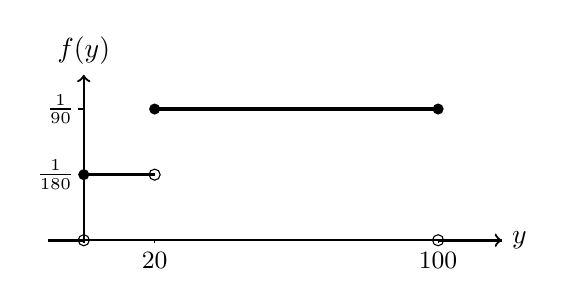
\begin{tikzpicture}[xscale=0.45, yscale=15]

\draw[->, thick] (-1,0) -- (11.8,0) node[right] {$y$};
\draw[->, thick] (0,-0.002) -- (0,0.14) node[above] {$f(y)$};

  \draw (2,0) -- (2,-0.002) node[below] {\small $20$};
    \draw (10,0) -- (10,-0.002) node[below] {\small $100$};

\draw (-0.15,1/18) -- (0,1/18) node[left] {\small $\frac{1}{180}$};
\draw (-0.15,1/9)  -- (0,1/9)  node[left] {\small $\frac{1}{90}$};

\draw[very thick] (-1,0) -- (0,0);
\draw[very thick] (10,0) -- (11.8,0);
\draw[very thick] (0,1/18) -- (2,1/18);
\draw[very thick] (2,1/9) -- (10,1/9);

\node[circle, draw=black, inner sep=0pt, minimum size=4pt] at (0,0) {};
\node[circle, fill=black, inner sep=0pt, minimum size=4pt] at (0,1/18) {};
\node[circle, draw=black,  inner sep=0pt, minimum size=4pt] at (2,1/18) {}; 
\node[circle, fill=black, inner sep=0pt, minimum size=4pt] at (2,1/9) {};
\node[circle, fill=black, inner sep=0pt, minimum size=4pt] at (10,1/9) {};
\node[circle, draw=black, inner sep=0pt, minimum size=4pt] at (10,0) {};

\end{tikzpicture}
    }
\end{minipage}

\part[5] Quelle est l'espérance de $Y$?

\begin{solution}
\begin{align*}
    E(Y)&=\int_{-\infty}^{\infty}yf_Y(y)dy\\
    &= \int_0^{20}\frac{x}{180}dx+\int_{20}^{100}\frac{x}{90}dx\\
    &=\frac{1}{360}[x^2]_{0}^{20}+ \frac{1}{180}[x^2]_{20}^{100}\\
    &= \frac{10}{9}+\frac{160}{3}\\
    &=\frac{490}{9}
\end{align*}    
\end{solution}
\end{parts}
\end{H26}

\begin{H26r}
\question (H26r)  Soit $X$ une variable aléatoire continue dont la fonction de répartition est donnée par
\[ F_X(x) = \begin{cases}
\displaystyle 0 & \mbox{si } x < 0, \\[6pt]
\displaystyle \frac{x^3}{8} & \mbox{si } 0 \le x < 2, \\[6pt]
\displaystyle 1 & \mbox{si } x \ge 2.
\end{cases} \]

\begin{parts}
    \part[4] Calculez $\mathbb{P}\!\left(X > 1 \;\middle|\; X < \dfrac{3}{2}\right)$.

    \begin{solution}
    \begin{align*}
    \mathbb{P}\!\left(X > 1 \mid X < \tfrac{3}{2}\right)
    &= \frac{\mathbb{P}\!\left(1 < X < \frac{3}{2}\right)}{\mathbb{P}\!\left(X < \frac{3}{2}\right)}
    = \frac{F_X\!\left(\frac{3}{2}\right) - F_X(1)}{F_X\!\left(\frac{3}{2}\right)}.
    \end{align*}

    On calcule:
    \[
    F_X\!\left(\tfrac{3}{2}\right) = \frac{(3/2)^3}{8} = \frac{27}{64}, \qquad
    F_X(1) = \frac{1}{8} = \frac{8}{64}.
    \]
    Donc
    \[
    \mathbb{P}\!\left(X > 1 \mid X < \tfrac{3}{2}\right)
    = \frac{\frac{27}{64} - \frac{8}{64}}{\frac{27}{64}}
    = \frac{19}{27}.
    \]
    \end{solution}
    

    \part[4] Trouvez la fonction de densité $f_X(x)$.

    \begin{solution}
    On dérive la fonction de répartition:
    \[
    f_X(x) = F_X'(x) = \begin{cases}
    \displaystyle \frac{3x^2}{8} & \mbox{si } 0 \le x < 2, \\[6pt]
    0 & \mbox{sinon.}
    \end{cases}
    \]
    \end{solution}
    

    

    \part[4] Calculez $\mathbb{E}(X)$.

    \begin{solution}
    \begin{align*}
    \mathbb{E}(X)
    &= \int_0^2 x \cdot \frac{3x^2}{8}\,dx
    = \frac{3}{8}\int_0^2 x^3\,dx
    = \frac{3}{8}\left[\frac{x^4}{4}\right]_0^2
    = \frac{3}{8} \cdot \frac{16}{4}
    = \frac{3}{2}.
    \end{align*}
    \end{solution}
\end{parts}
\end{H26r}


\moduleheader{mod3}{Module 3 - Lois discrètes}

\begin{H23}
\question (H23) Jean est un vendeur dans une boutique et à chaque fois qu'un client se présente, Jean a une chance sur 5 d'effectuer une vente. 

\begin{parts}
    \part[4] Quelle est la probabilité de conclure 2 ventes avec les 5 prochains clients?
    \begin{solution}
    Soit $X$ le nombre de ventes parmi 5 clients. $X \sim \text{Bin}(5, 1/5)$.
    \begin{align*}
    \mathbb{P}(X=2) &= \binom{5}{2} \left(\frac{1}{5}\right)^2 \left(\frac{4}{5}\right)^3
    = 10 \cdot \frac{1}{25} \cdot \frac{64}{125}
    = \frac{640}{3125} = \frac{128}{625}
    \end{align*}
    \end{solution}
    
    \part[4] Quelle est la probabilité que le premier client avec qui Jean conclut une vente soit le deuxième ou le troisième client qui s'est présenté à la boutique?
    \begin{solution}
    Soit $Y$ le numéro du client avec qui Jean conclut sa première vente. $Y \sim \text{Géom}(1/5)$.
    \begin{align*}
    \mathbb{P}(Y=2) + \mathbb{P}(Y=3) &= \left(\frac{4}{5}\right)^1\frac{1}{5} + \left(\frac{4}{5}\right)^2\frac{1}{5}\\
    &= \frac{4}{25} + \frac{16}{125}\\
    &= \frac{20}{125} + \frac{16}{125} = \frac{36}{125}
    \end{align*}
    \end{solution}
    
    \part[4] Quelle est la probabilité de devoir servir 8 clients pour effectuer deux ventes?
    \begin{solution}
    Soit $W$ le nombre de clients nécessaires pour obtenir 2 ventes. $W \sim \text{BinNég}(2, 1/5)$.
    \begin{align*}
    \mathbb{P}(W=8) &= \binom{8-1}{2-1} \left(\frac{1}{5}\right)^2 \left(\frac{4}{5}\right)^{6}\\
    &= 7 \cdot \frac{1}{25} \cdot \frac{4096}{15625}\\
    &= \frac{28672}{390625}
    \end{align*}
    \end{solution}
\end{parts}
\end{H23}

\begin{A23}
\question (A23)  Un enfant accepte de jouer au aux dominos avec son père jusqu'à ce qu'il perde une partie. L'enfant perd 9 parties sur 10, en moyenne. Soit $W$, le nombre de parties jouées, quelle est la loi de $W$? \textit{Ici, la loi de Pascal fait référence à la loi binomiale négative.}

\begin{checkboxes}
    \choice $W\sim$Bernoulli$(n=10, p=\sfrac{9}{10})$
    \choice $W\sim$Bernoulli$(p=\sfrac{9}{10})$
    \choice $W\sim$Binomiale$(n=10, p=\sfrac{9}{10})$
    \choice $W\sim$Binomiale$(p=\sfrac{9}{10})$
    \choice $W\sim$Géométrique$(n=10, p=\sfrac{9}{10})$
    \correctchoice $W\sim$Géométrique$(p=\sfrac{9}{10})$
    \choice $W\sim$Poisson$(\lambda=\sfrac{9}{10})$
    \choice $W\sim$Pascal$(r=10, p=\sfrac{9}{10})$
    \choice $W\sim$Pascal$(p=\sfrac{9}{10})$

\end{checkboxes}
\end{A23}

\begin{A23}
\question (A23) La lune suscite un grand intérêt pour les pêcheurs car la qualité de la pêche dépend directement des différentes phases lunaires. Un pêcheur a remarqué les faits suivants pour chaque période d'une heure de pêche:

\begin{itemize}
    \item Lorsque la lune est croissante, la probabilité de pêcher au moins un poisson est de cinq sur sept;
    \item Lorsque la lune est décroissante, la probabilité de ne pêcher aucun poisson est de deux sur cinq.
\end{itemize}
La lune est considérée la moitié du temps comme croissante, et l'autre moitié comme décroissante.

\begin{parts}
    \part[3] Quelle est la probabilité qu'en pêchant une heure, le pêcheur pêche au moins un poisson?

\part[3] Si le pecheur ne pêche aucun poisson après une heure de pêche, quelle est la probabilité que la lune soit croissante?

\part[3] Si, en période de lune croissante, il pêche trois heures de suite, quelle est la probabilité qu'il ne pêche aucun poisson?

\part[3] Si, en période de lune décroissante, il pêche aussi trois heures de suite, quelle est la probabilité qu'il pêche au moins un poisson ?
\end{parts}

 .
\end{A23}

\begin{A24}
\question (A24) Un joueur de fléchette atteint la cible centrale avec une probabilité de 0.05. On suppose que les lancers sont indépendants.

\begin{parts}
    \part[4] Calculez la probabilité qu’il atteigne la cible pour la première fois au septième lancer.

\begin{solution}
    Soit la variable aléatoire:

    X= le nombre de lancers nécessaires pour atteindre la cible pour la première fois.

    X suit une loi géométrique de paramètre 0.05.

    D'où
    $$P(X=7)=0.05(1-0.05)^6 = 0.03675$$
\end{solution}

\part[4] Calculez la probabilité qu’il atteigne la cible pour la deuxième fois au dixième lancer. 
\begin{solution}
    Soit la variable aléatoire:

    X= le nombre de lancers nécessaires pour atteindre la cible pour la deuxième fois.

    X suit une loi de Pascal de paramètre $r=2$ et $p=0.05$.

    D'où
    $$P(X=10)=\binom{9}{1}0.05^2(1-0.05)^9 = 0.015$$
\end{solution}

\end{parts}
\end{A24}

\begin{H25}
\question (H25) Un vendeur d’ordinateurs a constaté que 30\% des clients qui entrent dans son magasin, faisaient l’achat d’un ordinateur et que les clients achètent les ordinateurs indépendamment les uns des autres.
Définissez clairement les variables aléatoires qui interviennent dans vos calculs pour répondre aux questions suivantes.
\begin{parts}
\part [4] Quatre clients sont dans le magasin. Quelle est  la probabilité qu’au moins un d’entre eux achète un ordinateur?  

\part [4] Calculez la probabilité que 4 clients doivent entrer dans le magasin pour que le magasin vende son premier ordinateur? 

\part [4] Combien de clients, en moyenne, doivent entrer dans le magasin pour que le magasin vende son troisième ordinateur?  
\end{parts}
\end{H25}

\begin{H25}
\question (H25) Les avions d’une grande compagnie aérienne atterrissent, dans un aéroport très achalandé, selon une loi de Poisson avec une moyenne de six avions à l’heure.

Définir clairement les variables aléatoires qui interviennent dans vos calculs pour répondre aux questions suivantes.
\begin{parts}
\part [4] Calculez la probabilité de voir atterrir 2 avions ou plus en 15 minutes.

\part [4] Calculez la probabilité de devoir attendre plus de 20 minutes pour voir atterrir un avion. 

\part [4] Combien de temps, en moyenne, devriez-vous attendre pour voir atterrir, dans cet aéroport,  le cinquième avion de cette compagnie.
\end{parts}
\end{H25}

\begin{A25}
\question (A25) 
L'examen du code de la route comporte 40 questions. Chaque question propose $4$ réponses possibles, dont une seule est correcte. Pour chaque question, le candidat connaît la bonne réponse avec probabilité $p$. S'il connaît la réponse, il répond correctement avec certitude. S'il ne la connaît pas, il choisit alors une réponse au hasard parmi les 4 possibilités. On suppose que les questions sont indépendantes.

Pour $1 \le i \le 40$, on définit l'événement 
\begin{align*}
   A_i = \{\text{le candidat répond correctement à la $i$-ème question}\}. 
\end{align*}
On note $S$ le nombre total de bonnes réponses.

\begin{parts}
    \part[6] Calculez $P(A_i)$ en fonction de $p$ pour $1 \le i \le 40$.\\
\\
\begin{solution}
    
Pour une question donnée $i$, on distingue deux cas :
    \begin{itemize}
        \item Le candidat connaît la réponse (probabilité $p$) et répond alors correctement avec probabilité 1.
        \item Le candidat ne connaît pas la réponse (probabilité $1-p$) et choisit uniformément parmi les 4 réponses,
        donc avec probabilité $1/4$ de tomber sur la bonne.
    \end{itemize}
    Ainsi, 
    \[
    P(A_i) = p \cdot 1 + (1-p)\cdot \frac{1}{4}
    = \frac{1}{4} + \frac{3}{4}\,p.
    \]
    \end{solution}
    
    
    \part[6] Déterminez la loi de $S$ (en justifiant votre réponse).
    \\
    \\
    \begin{solution}
        
    Les événements $A_i$ sont indépendants et identiquement distribués (même probabilité de succès $P(A_i)$).
    La variable aléatoire $S$ est donc une somme de 40 variables de Bernoulli de paramètre
    \[
    P(A_i) = \frac{1}{4} + \frac{3}{4}p.
    \]
    On en déduit :
    \[
    S \sim \mathrm{Binomiale}\bigl(40,\; \tfrac{1}{4} + \tfrac{3}{4}p \bigr).
    \]

    \end{solution}

\end{parts}
\end{A25}

\begin{A25}
\question (A25) 
On effectue un contrôle de fabrication sur des pièces dont une proportion $p=0.02$ est défectueuse. 

\begin{parts}
    \part[4] On contrôle un lot de $1000$ pièces: Soit $X$ la variable aléatoire : « nombre de pièces défectueuses parmi $1000$ ». 
    Quelle est la loi de $X$ ? 

    \begin{solution}
        
    
    On a $X \sim \text{Binomiale}(n=1000, p=0.02)$. \\
    Espérance : $\mathbb{E}[X] = np = 1000 \times 0.02 = 20$. \\
    Variance : $\mathrm{Var}(X) = np(1-p) = 1000 \times 0.02 \times 0.98 = 19.6$. \\
    Écart-type : $\sigma_X = \sqrt{19.6} \approx 4.43$.
    \end{solution}

    \part[4] En approximant cette loi par celle d’une loi normale, calculez la probabilité que $X$ soit compris entre $18$ et $22$. 

    \begin{solution}
        
    
    Approximation normale : $X \approx \mathcal{N}(20, 19.6)$. \\
    Sans correction de continuité : \\
    $\mathbb{P}(18 \leq X \leq 22) \approx \mathbb{P}\!\left(\frac{18-20}{4.43} \leq Z \leq \frac{22-20}{4.43}\right) = \mathbb{P}(-0.45 \leq Z \leq 0.45)\approx 2\Phi(0.45)-1 \approx 0.349.$ \\
    Avec correction de continuité : \\
    $\mathbb{P}(18 \leq X \leq 22) \approx \mathbb{P}\!\left(\frac{17.5-20}{4.43} \leq Z \leq \frac{22.5-20}{4.43}\right) = \mathbb{P}(-0.56 \leq Z \leq 0.56)\approx 2\Phi(0.56)-1 \approx 0.428.$
    \end{solution}
\end{parts}
\end{A25}

\begin{A25}
\question (A25)  Une personne a $n$ clés sur son porte-clés.
Parmi ces $n$ clés, $k$ clés déverrouillent une même serrure. 
La personne tente de déverrouiller cette serrure en utilisant une succession de clés, avec remise, c'est-à-dire qu'après avoir tenté avec une clé qui ne fonctionne pas, la clé est remise dans le lot.
On note $X$ la variable aléatoire du nombre de clés testées avant que la serrure soit déverrouillée.
Que vaut $P(X=k)$?

\begin{oneparcheckboxes}
    \choice $\displaystyle \left(\frac{n-k}{n}\right)^{k-1}\frac{k}{n}$
    \choice $\displaystyle \binom{n}{k}\left(\frac{k}{n}\right)^{k}\left(1-\frac{k}{n}\right)^{n-k}$
    \correctchoice $\displaystyle \binom{k-1}{n-1}\left(\frac{k}{n}\right)^{n}\left(1-\frac{k}{n}\right)^{n-k}$
    \choice $\displaystyle \frac{k}{n}$
\end{oneparcheckboxes}
\end{A25}

\begin{H26}
\question (H26) 

Une voiture est stationnée sans avoir payé. Chaque jour, indépendamment des autres jours, il y a une probabilité \(p=0{,}15\) qu’elle reçoive une contravention.
On suppose qu’au plus une contravention peut être donnée par jour.
Le coût d’une contravention est de \(65\$\). Le coût d’un permis de stationnement mensuel est de \(180\$\).

\begin{parts}
\part[4] Quelle est la probabilité que la voiture ne reçoive \emph{aucune} contravention au cours des \(7\) premiers jours?
\begin{solution}
Sur \(7\) jours, le nombre de contraventions $X$ suit une loi binomiale :
\[
X \sim \text{Bin}(7,0{,}15).
\]
Donc
\[
\mathbb{P}(X=0)=\binom{7}{0}(0{,}15)^0(0{,}85)^7=(0{,}85)^7.
\]   
\end{solution}

\part[4] Après combien de jours s’attend-on, en moyenne, à recevoir la première contravention?
\begin{solution}
 Le nombre de jours avant la première contravention suit une loi géométrique de paramètre \(p=0{,}15\).
Ainsi, le nombre moyen de jours avant la première contravention est
\[
\frac{1}{p}=\frac{1}{0{,}15}=\frac{20}{3}\approx 6{,}67\ \text{jours}.
\]   
\end{solution}

\part[4] En moyenne, après combien de jours s’attend-on à ce que le total des contraventions atteigne ou dépasse \(180\$\)?
\begin{solution}
    Atteindre ou dépasser \(180\$\) nécessite au moins \(3\) contraventions, car
\[
2\times 65=130<180
\qquad \text{et} \qquad
3\times 65=195\ge 180.
\]

On cherche donc le nombre moyen de jours pour recevoir \(3\) contraventions.

Le nombre de jours nécessaires pour obtenir \(r=3\) succès, lorsque chaque jour est un essai indépendant de probabilité \(p=0{,}15\), suit une loi de Pascal (binomiale négative).
Pour cette loi, l’espérance du nombre d’essais nécessaires pour obtenir \(r\) succès est
\[
\mathbb{E}(\text{jours})=\frac{r}{p}.
\]

Ainsi,
\[
\mathbb{E}(\text{jours})=\frac{3}{0{,}15}=20.
\]

\[
\boxed{\text{En moyenne, cela devrait prendre } 20 \text{ jours.}}
\]
\end{solution}
\end{parts}
\end{H26}

\begin{H26}
\question (H26) 

Dans un projet de cartographie, un drone envoie automatiquement des relevés de position vers un serveur. Les relevés sont reçus indépendamment les uns des autres, à un taux constant au cours du temps. On suppose que le nombre de relevés reçus suit un processus de Poisson de taux \(\lambda = 1{,}5\) relevé par heure. Charles surveille la réception des relevés.

\begin{parts}
\part[4]  Charles souhaite aller dîner pendant \(40\) minutes.
Quelle est la probabilité qu’il ne manque \emph{aucun} relevé pendant son absence? 
\begin{solution}
Sur \(40\) minutes, soit \(t=\frac{40}{60}=\frac{2}{3}\) heure, le nombre de relevés reçus suit une loi de Poisson
de paramètre
\[
\lambda t = 1{,}5 \times \frac{2}{3} = 1.
\]
Ainsi,
\[
\mathbb{P}(\text{aucun relevé}) = \mathbb{P}(X=0) = e^{-1}.
\]
\end{solution}

\part[4] S’il vient de recevoir un relevé, en moyenne combien de temps a-t-il
avant de recevoir le \emph{prochain} relevé?
\begin{solution}
Le temps d’attente avant la réception du prochain relevé suit une loi exponentielle
de paramètre \(\lambda = 1{,}5\).
L’espérance vaut
\[
\frac{1}{\lambda} = \frac{1}{1{,}5} = \frac{2}{3}\ \text{heure},
\]
soit environ \(40\) minutes.

\end{solution}

\part[4] Pour rédiger son article, Charles a besoin de  \(100\) relevés. En moyenne, combien de temps faudra-t-il pour obtenir ces \(100\) relevés?
\begin{solution}
Le temps nécessaire pour recevoir \(100\) relevés suit une loi gamma
de paramètre de forme \(k=100\) et de taux \(\lambda = 1{,}5\).
L’espérance vaut
\[
\frac{k}{\lambda} = \frac{100}{1{,}5} \approx 66{,}7\ \text{heures}.
\]
\end{solution}
\end{parts}
\end{H26}

\begin{H26r}
\question (H26r) 

On peut modéliser le nombre de jours avant la panne d'un serveur informatique par une loi géométrique de paramètre $p=0{,}4$. Après 10 jours sans panne, que peut-on dire?

\begin{checkboxes}
\choice La panne est maintenant plus probable qu'au début.
\choice La panne est moins probable qu'au début.
\correctchoice La probabilité de panne demain est la même qu'au premier jour.
\choice Il est certain qu'une panne surviendra bientôt.
\end{checkboxes}
\begin{solution}
La loi géométrique possède la propriété d'absence de mémoire~: $\mathbb{P}(X > s+t \mid X > s) = \mathbb{P}(X > t)$. Le fait d'avoir survécu 10 jours sans panne ne change pas la probabilité de panne le lendemain.
\end{solution}
\end{H26r}

\begin{H26r}
\question (H26r) 

Dans un projet de cartographie, un drone tente d’envoyer des relevés de
position vers un serveur. À chaque tentative, le relevé est soit reçu
avec succès, soit perdu. On suppose que les tentatives sont indépendantes
et que la probabilité qu’un relevé soit reçu avec succès est constante et
égale à $p=0{,}6$.

Charles surveille la réception des relevés.

\begin{parts}

\part[4]
Au cours des $10$ prochaines tentatives, quelle est la probabilité que
\emph{exactement $7$} relevés soient reçus avec succès?

\begin{solution}
Soit $X$ le nombre de relevés reçus avec succès parmi $10$ tentatives.
Alors
\[
X \sim \text{Binomiale}(10,0{,}6).
\]
On a donc
\[
\mathbb P(X=7)
= \binom{10}{7}(0{,}6)^7(0{,}4)^3.
\]
\end{solution}

\part[4]
Quelle est la probabilité que le \emph{premier} relevé reçu avec succès
survienne à la $5^{\text{e}}$ tentative?

\begin{solution}
Soit $T$ le numéro de la tentative correspondant au premier succès.
Alors
\[
T \sim \text{Géométrique}(0{,}6).
\]
On obtient
\[
\mathbb P(T=5)=(1-0{,}6)^4(0{,}6)=(0{,}4)^4(0{,}6).
\]
\end{solution}

\part[4]
Chaque tentative d’envoi coûte $0{,}40\$$, qu’elle soit réussie ou non.
De plus, le lancement du drone entraîne un coût fixe de $10\$$.
On souhaite obtenir $50$ relevés reçus avec succès. On note $Z$ le coût total (en dollars) nécessaire pour atteindre cet
objectif. Calculez $\mathbb E[Z]$.

\begin{solution}
Soit $Y$ le nombre de tentatives nécessaires pour obtenir $50$ relevés
reçus avec succès. Comme chaque tentative est indépendante et que la
probabilité de succès est $p=0{,}6$, on a
\[
Y \sim \text{Pascal}(50,0{,}6).
\]

Pour une loi de Pascal de paramètres $(r,p)$, l’espérance est
\[
\mathbb E[Y] = \frac{r}{p}.
\]
Ainsi,
\[
\mathbb E[Y] = \frac{50}{0{,}6} \approx 83{,}33.
\]

Le coût total s’écrit
\[
Z = 10 + 0{,}40\,Y.
\]
Par linéarité de l’espérance,
\[
\mathbb E[Z]
= 10 + 0{,}40\,\mathbb E[Y]
= 10 + 0{,}40 \times \frac{50}{0{,}6}.
\]
Numériquement,
\[
\mathbb E[Z] \approx 10 + 33{,}33 = 43{,}33\ \text{\$}.
\]
\end{solution}

\end{parts}
\end{H26r}

\begin{H26r}
\question (H26r) Dites si les énoncés suivants sont vrais ou faux. Aucune justification n'est requise.

\begin{parts}

    \part[1] Si $X \sim \mathrm{Bin}(n, p)$, alors $E(X) = np$ et $\mathrm{Var}(X) = np(1-p)$.

    \begin{oneparcheckboxes}
        \correctchoice Vrai
        \choice Faux
    \end{oneparcheckboxes}

    \begin{solution}
    Vrai. Ce sont les formules classiques de l'espérance et de la variance de la loi binomiale.
    \end{solution}

    \part[1] Si $X \sim \mathrm{Exp}(\lambda)$, alors $\mathrm{Var}(X) = \lambda^2$.

    \begin{oneparcheckboxes}
        \choice Vrai
        \correctchoice Faux
    \end{oneparcheckboxes}

    \begin{solution}
    Faux. Pour une loi exponentielle de paramètre $\lambda$, on a $\mathrm{Var}(X)=\dfrac{1}{\lambda^2}$ (et $E(X)=\dfrac{1}{\lambda}$).
    \end{solution}

\end{parts}
\end{H26r}


\moduleheader{mod4}{Module 4 - Lois continues, processus de Poisson et loi normale}

\begin{A22}
\question (A22)  Si $X$ est une variable aléatoire normale de moyenne $\mu$ et de variance $\sigma^2$, nous pouvons écrire $X\sim\mathcal{N}(\mu, \sigma^2)$. Laquelle des affirmations suivantes est vraie? 

\begin{checkboxes}
\choice $\displaystyle Z=\frac{X-\mu}{\sigma^2}\sim \mathcal{N}(0, 1)$
\choice $\displaystyle Y=3X+2 \sim \mathcal{N}(3\mu+2, 9\sigma^2 + 4)$
\CorrectChoice La fonction de densité de $X$ est symétrique
\choice La fonction de répartition de $X$ est symétrique
\end{checkboxes}
\end{A22}

\begin{A22}
\question (A22) Un producteur de Vacherin Fribourgeois sait que le poids d'une de ses meules de fromage, $X$, est une variable aléatoire de loi normale $\mu=15$ kg et $\sigma^2 = 4$ kg$^2$.

\begin{parts}
    \part[6] Quelle est le poids $p$, tel que $P(X>p)=0,15866$? Laissez des traces de votre démarche.
    \begin{solution}
        On cherche $P(X>p)=0,15866$ sachant que $X\sim\mathcal{N}(15, 4)$
        \begin{align*}
            P(X>p)&= P\left(\frac{X-15}{2}>\frac{p-15}{2}\right)\\
            0,15866&= P\left(Z>\frac{p-15}{2}\right) \ \ \text{ où } Z\sim \mathcal{N}(0,1)\\
            1-0,15866 &= P\left(Z\leq\frac{p-15}{2}\right)\\
           1-0,15866 &= \Phi\left(\frac{p-15}{2}\right)\\
           0,84134 &= \Phi\left(\frac{p-15}{2}\right)\\
           \Phi^{-1}(0,84134) &= \frac{p-15}{2}\\
           1&= \frac{p-15}{2}\\
           p &= 17
        \end{align*}
    \end{solution}
    
    \part[8] Le producteur doit envoyer 100 meules à un supermarché. Une compagnie de transport lui charge 1500\$ si le poids des 100 meules est inférieur à 1800 kg ou 2000\$ si le poids est supérieur ou égal à 1800~kg. Quelle est l'espérance du prix que le producteur devra payer pour le transport avec cette compagnie? Laissez des traces de votre démarche.

    \begin{solution}
     Soit $Y=X_1+...+X_100$, $Y\sim\mathcal{N}(100*15; 100*4)$, $Y\sim\mathcal{N}(1500, 400)$.
     
     On commence par trouver la probabilité que $Y>1800$. 
     \begin{align*}
         P(Y>1800)&= P(Z>\frac{1800-1500}{20})\\
         &= P(Z>15)\\
         &\approx 0
     \end{align*}
     
     Soit $W$ la variable qui décrit si le poids est supérieur à 1800kg, $W\sim$Bernoulli$(\approx 0)$. On sait que $E(W)\approx0$.
     
     Soit $T$ qui décrit le prix que payera le producteur, $T=1500+500W$. D'où $E(T)=1500+500E(W)\approx 1500$

     OU

     $E(T)\approx1500 * 1+2000 * 0$. Il s'agit de la somme sur les possibilité de $T$ multiplié par la probabilité (l'espérance...).
    \end{solution}
    
\end{parts}
\end{A22}

\begin{A22}
\question (A22) Le nombre de tentatives d'infiltration dans un serveur sécurisé se fait selon un processus de Poisson. Le temps moyen entre deux tentatives est $12$ minutes. 
\begin{parts}
    \part[5] Quelle est la probabilité que le temps entre deux tentatives soit supérieur à $20$ minutes. Laissez des traces de votre démarche.
\begin{solution}
    Si le temps moyen $X$ entre deux tentatives est de 12 minutes, $X\sim \exp(\lambda = 1/12)$. D'où 

    \begin{align*}
        P(X>20)&=\int _{20}^\infty \frac{1}{12}\exp\left(\frac{-x}{12}\right)dx\\
        &= \left.-\exp\left(\frac{-x}{12}\right)\right|_{20}^\infty\\
        &= \exp\left(-20/12\right)\\
        &\approx 0,189.
    \end{align*}

    OU DIRECTEMENT

        \begin{align*}
        P(X>20)&=1-[1-\exp\left(-20/12\right)] \text{ par la fonction de répartition }\\
        &\approx 0,189.
    \end{align*}

    OU 

    Si le temps moyen entre deux tentatives est de 12 minutes, il s'agit d'un processus de Poisson d'intensité 1 tentative / 12 minutes. Sur 20 minutes, le \# de tentatives $Y$ suit donc une Poisson($\mu = 5/3$). On cherche donc $P(Y=0)$.

    \begin{align*}
        P(Y=0) &= \frac{\exp(-5/3)\left(\frac{-5}{3}\right)^0}{0!}\\
        &= \exp(-5/3)\\
        &\approx 0,189
    \end{align*}
    
\end{solution}

    

    

    \part[5] Une équipe d'experts tente de répliquer les tentatives d'infiltration dans le but d'améliorer les défenses du serveur. Ils lancent une séquence de tentatives d'infiltration selon le même processus de Poisson. Quelle est l'espérance du temps total pour lancer les 8 tentatives d'infiltration? Justifiez votre réponse.
    \begin{solution}
        Si $W$ est le temps pour lancer 8 tentatives, $W\sim \text{Gamma}(8; 1/12)$, donc $E(W)=\frac{8}{1/12}=96$ minutes.
    \end{solution}
\end{parts}
\end{A22}

\begin{A22}
\question (A22)  Yasmine s'intéresse à une variable aléatoire $X$ suivant une loi Binomiale($n=70,p=0,3$). Elle souhaite calculer ${P( 18 < X < 35)}$, mais n'a pas accès à un ordinateur et n'a pas envie de faire tous les calculs à la main. En utilisant la méthode présentée en classe, calculez approximativement cette probabilité. 

\begin{solution}
On approxime la loi binomiale avec la loi normale, en utilisant la correction pour la continuité.\\

On s'intéresse à $X = \sum_{i=1}^n X_i$ où chaque $X_i$ suit une loi Bernoulli(p).\\
On sait donc que $E(X_i) = p =0.3$ et $V(X_i) = p(1-p)=0.3*0.7=0.21$. \\
Le théorème central limite nous indique que $X \approx N(\mu = 70*0,3=21 ;  \sigma^2= 70*0.21=14,7$). 

En utilisant la correction pour la continuité, on doit calculer $$P(17,5 \le X \le 35,5) \mbox{ où } X \sim N(21; 17,4).$$

On commence par standardiser: 
\begin{align*}
P(17,5 \le X \le 35,5) &= P\left(\frac{17,5-21}{\sqrt{17,4}} \le \frac{X-21}{\sqrt{17,4}} \le \frac{35,5-21}{\sqrt{17,4}}\right) \\
&= P( -0,839 \leq Z \leq 3,47) 
\end{align*}

On utilise maintenant la table de la loi normale:
\begin{align*}
P( -0,839 \leq Z \leq 3,47) & = P(Z \leq 3,47) - P(Z \leq -0,839) \\
& = 0,99974 - (1-0,79954) = 0,79928
\end{align*}

\end{solution}
\end{A22}

\begin{A22}
\question (A22) 

Le poids des tomates d’un agriculteur suit une loi normale de moyenne $300$ grammes
et de variance $100$ grammes$^2$. On prend des mesures sur 25 tomates choisies aléatoirement et on obtient une moyenne échantillonnale de 309 grammes et une variance échantillonnale de 118 grammes$^2$.
Est-ce que la valeur de 118 grammes$^2$ est un paramètre ou une statistique ?

\begin{oneparcheckboxes}
\choice Un paramètre
\choice Une statistique
\end{oneparcheckboxes}
\end{A22}

\begin{H23}
\question (H23) Un médecin reçoit en moyenne 6 patients par heure. 

\begin{parts}
    \part[4] Quelle est la probabilité que 2 patients rentrent voir le médecin durant les 30 prochaines minutes ?
    \begin{solution}
    Processus de poisson d'intensité 1 patient / 10 minutes.\\
    $X$: nombre de patients par 30 minutes\\
    $X\sim$Poisson($\mu=1 \cdot 30 / 10$), donc $X\sim$Poisson($\mu=3$).\\
    On cherche $P(X=2) = \displaystyle\frac{3^2e^{-3}}{2!}= \frac{9e^{-3}}{2}$
    
    \end{solution}
    
    \part[4] Vous êtes le premier sur la liste des patients, quelle est la probabilité que vous attendiez plus que 12 minutes avant de voir le médecin ?
    \begin{solution}
     Processus de poisson d'intensité 1 patient / 10 minutes.\\
        $Y$: temps entre deux patients\\
        $Y\sim$Exp($\frac{1}{10}$)\\
        On cherche $P(Y>12)=1-(1-e^{-12/10})=e^{-6/5}$
    \end{solution}
    
    \part[4] Dans combien de temps la cinquième personne sur la liste d'attente peut-elle espérer voir le médecin?
    \begin{solution}
      Processus de poisson d'intensité 1 patient / 12 minutes.\\
    $W$: temps avant le 5e patient\\
    $W\sim$Gamma($5, \frac{1}{10}$)\\
    On cherche $\mathbb{E}(W)=5\cdot10=50$
    \end{solution}
\end{parts}
\end{H23}

\begin{H23}
\question (H23) Soient $X_1$, $X_2$ et $X_3$ trois variables aléatoires indépendentes telles que 
\begin{itemize}
\item $X_1 \sim {\cal N}(1,2)$
\item $X_2 \sim {\cal N}(0,3)$
\item $X_3 \sim {\cal N}(1,1)$
\end{itemize}
On pose $Y=X_1+X_2+2 X_3$.

\begin{parts}
    \part[3] Donner la loi de $Y$.
    \begin{solution}
    Puisque $X_1, X_2, X_3$ sont indépendantes et normales, $Y = X_1 + X_2 + 2X_3$ est aussi normale.
    \begin{align*}
    \mathbb{E}(Y) &= \mathbb{E}(X_1) + \mathbb{E}(X_2) + 2\mathbb{E}(X_3) = 1 + 0 + 2(1) = 3\\
    \text{Var}(Y) &= \text{Var}(X_1) + \text{Var}(X_2) + 4\,\text{Var}(X_3) = 2 + 3 + 4(1) = 9
    \end{align*}
    Donc $Y \sim \mathcal{N}(3, 9)$.
    \end{solution}
    
    \part[4] Calculer $\mathbb{P}(0 \le Y \le 6)$.
    \begin{solution}
        Comme $Y\sim\mathcal{N}(3, 9)$\\
        \begin{align*}
            P(0\leq Y \leq 6) &= P\left(\frac{0-3}{3}\leq Z \leq \frac{6-3}{3}\right)\\
            =& P(-1\leq Z \leq 1)\\
            =& 2 \Phi(1) - 1\\
            =& 2\cdot 0,84134 - 1\\
            =&0,68268
        \end{align*}
    \end{solution}
    \part[4] Trouver $m$ tel que $\mathbb{P}(Y>m)=0.4$.
    \begin{solution}
        On cherche $m$ t.q. $P(Y>m=0,4)$ ou $1-P(Y\leq m) =0,4$, donc
        \begin{align*}
            P(Y\leq m) =& 0,6\\
            P\left(Z\leq \frac{m-3}{3}\right)=&0,6\\
        \end{align*}
        On trouve donc que $\displaystyle\frac{m-3}{3}=0,25$, donc $m=3,75$ (réponses entre 3,75 et 3,78 acceptées).
    \end{solution}
\end{parts}
\end{H23}

\begin{A23}
\question (A23)  \label{A23-I8-CDF} La variable aléatoire $X$ suit une loi normale d'espérance $\mu$ et de variance $\mu^4$.

Sachant que $P(X\leq 0)= 0,84134$ et que $P(X>1)=0,002275$, que vaut $\mu_X$?

 .
\end{A23}

\begin{A23}
\question (A23) Un employé d'un centre d'appel reçoit en moyenne 8 appels par heure. Pour chacune des sous-questions de cet exercice, vous aurez 1 point si vous identifiez la bonne loi et son(ses) paramètre(s).

\begin{parts}
    \part[4] Quelle est la probabilité que l'employé reçoive 2 appels dans les 30 prochaines minutes ?
    \begin{solution}
    Processus de poisson d'intensité 1 patient / 10 minutes.\\
    $X$: nombre de patients par 30 minutes\\
    $X\sim$Poisson($\mu=1 \cdot 30 / 10$), donc $X\sim$Poisson($\mu=3$).\\
    On cherche $P(X=2) = \displaystyle\frac{3^2e^{-3}}{2!}= \frac{9e^{-3}}{2}$
    
    \end{solution}
    
    \part[4] L'employé a reçu 3 appels dans les 7 dernières minutes. Quelle est la probabilité que le prochain appel surviennent dans 10 minutes?
    \begin{solution}
     Processus de poisson d'intensité 1 patient / 10 minutes.\\
        $Y$: temps entre deux patients\\
        $Y\sim$Exp($\frac{1}{10}$)\\
        On cherche $P(Y>12)=1-(1-e^{-12/10})=e^{-6/5}$
    \end{solution}
    
    \part[4] L'employé a maintenant reçu 18 appels dans les 2 dernières heures. Quelle est l'espérance du temps avant que les 5 prochains appels surviennent?
    \begin{solution}
      Processus de poisson d'intensité 1 patient / 12 minutes.\\
    $W$: temps avant le 5e patient\\
    $W\sim$Gamma($5, \frac{1}{10}$)\\
    On cherche $\mathbb{E}(W)=5\cdot10=50$
    \end{solution}
\end{parts}
 . 
\bonusquestion[5]
Soit la variable aléatoire $X$ dont la fonction de répartition est donnée par

\begin{align*}
F_X(x)= \left\{
\begin{tabular}{l l}
$1- e^{-x}$,&\mbox{si $0\leq x$},\\
$0$,& \mbox{sinon},
\end{tabular}
\right.
\end{align*}
et la variable aléatoire $Y=aX+b$, où $a,b\in\mathbb{R}$.
Quelle est la fonction de répartition de Y?
\end{A23}

\begin{A24}
\question (A24) Le passage des voitures sur un certain viaduc est régi par un processus de Poisson d'intensité 60 par heure.

\begin{parts}
   \part[7] Quelle est la probabilité que la prochaine voiture passe dans plus de 12 minutes, sachant qu'aucune voiture ne passera dans les 6 prochaines minutes?
     \begin{solution}
     
     On peut résoudre de deux façons. 
     
     \textbf{Première façon:}
     
    Si on cherche une probabilité sur un intervalle de temps, la variable aléatoire $X$ qui mesure le temps entre deux événements suit une loi exponentielle de paramètre $\lambda=60$ (les unités sont des heures, si les étudiants ont transformé en minutes, ça marche).

    
Ici on cherche $P(X>\sfrac{1}{5}|X>\sfrac{1}{10})$. Comme la loi exponentielle est sans mémoire:
\begin{align*}
    P(X>\sfrac{1}{5}|X>\sfrac{1}{10}) &= P(X>\sfrac{1}{10})\\
    &= 1- (1-e^{-6})\\
    &= e^{-6}\\
    &\approx 0,0025
\end{align*}

     \textbf{Deuxième façon:}

On peut aussi dire que le nombre d'événements $Y$ sur un intervalle de 6 minutes suit une loi de Poisson de paramètre $\mu=\sfrac{1}{10}\times 60= 6$.

Nous cherchons donc $P(Y_2=0|Y_1=0)$, où $Y_1$ est sur le premier intervalle de 6 minutes et $Y_2$ est sur le deuxième intervalle. Ces deux variables aléatoires sont indépendantes.

\begin{align*}
    P(Y_2=0|Y_1=0)&= \frac{P(Y_2=0 \cap Y_1=0)}{P(Y_1=0)}\\
    &= \frac{P(Y_2=0 )P( Y_1=0)}{P(Y_1=0)}\\
    &= P(Y_2=0 )\\
    &= \frac{6^0e^{-6}}{0!}\\
    &= e^{-6}\\
    &\approx 0,0025
\end{align*}

    \end{solution}
   

   \part[3] Quelle est l'espérance du temps avant que 6 voitures passent sur le viaduc?
   \begin{solution}
       $W$, le temps avant que 6 voitures ne passent suit une loi Gamma de paramètres $n=6$ et $\lambda = 60$.
$$E(W)=\frac{n}{\lambda}=\frac{1}{10}$$

On peut donner 1/10e d'heure ou 6 minutes. Les étudiants doivent avoir mentionner qu'il s'agit d'une Gamma.
   \end{solution}
\end{parts}
\end{A24}

\begin{A24}
\question (A24) 
Soit trois éléments indépendants assemblés bout à bout. La longueur de chacun présente une 
distribution normale avec une moyenne de 2 pouces et un écart-type de 0,2 pouce. Or, les assemblages produits doivent avoir une longueur totale de 5,7 à 6,3 pouces. Quelle proportion d’entre eux satisfait à cette exigence ?

\begin{solution}
    Soient $X_i$ la variable aléatoire qui désigne la longueur de l'élément $i,\ i=1, 2, 3$.

    $X_i$ suit la loi normale de paramètres $\mu =2$ et $\sigma^2 =0.04$, par conséquent la longueur totale $Y=X_1+X_2+X_3$ suit la loi normale de paramètres $\mu =6$ et $\sigma^2 =0.12$.

 Donc
 $$
 \begin{array}{ccl}
     P(5.7\leq Y \leq 6.3) &=& P(\frac{5.7-6}{0.3464} < Z<\frac{6.3-6}{0.3464})  \\
      &=& \Phi(0.866) -  \Phi(-0.866) \\
      &=& 2 \Phi(0.866) -1 \\
      &=& 2(0.80785) -1 \\
      &=& 0.6157
 \end{array}
 $$
 \end{solution}
\end{A24}

\begin{H25}
\question (H25) Le diamètre $X$ (exprimé en cm) des tomates livrées à une usine d'emballage
américaine suit une loi normale $\mathcal{N}(7,\ \sigma^2)$ où l'écart-type $\sigma$ de $X$ est inconnu. Un tri automatique rejette
toutes les tomates dont le diamètre n'est pas compris entre 6 cm et 8 cm.
\begin{parts}
\part [6] On constate que 10\% des tomates livrées sont rejetées par ce procédé de tri.\\ Calculez l'écart type $\sigma$.

\part [6] Le  directeur  veut  réduire  à  5\%  le  pourcentage  de  tomates  rejetées  lors  du  tri.  Ne
pouvant  agir  sur  les  livraisons,  il  installe  un  système  de  tri  qui  rejette  les  tomates  de
diamètre inférieur à $7-s$ ou supérieur à $7+s$. \\
Calculez s.
\end{parts}
\end{H25}

\begin{H25}
\question (H25) Soit la variable aléatoire $X$ qui suit une loi uniforme sur l'intervalle $[a,b]$. Nous savons que $E(X)=4$ et $V(X)=3$. 

\begin{parts}
    \part[5] Donnez la fonction de densité de $X$.
\begin{solution}
    Il faut déduire $a$ et $b$ à partir de l'espérance et de la variance.

    Nous avons 
    \begin{align*}
        E(X)=&\frac{a+b}{2}\\
        4=&\frac{a+b}{2}\\
        \text{et} &\\
        V(X)=&\frac{(b-a)^2}{12}\\
        3=&\frac{(b-a)^2}{12}
    \end{align*}

    On déduit que $a=8-b$, donc $36 = (b-(8-b))^2=(2b-8)^2$. Il existe donc deux solutions pour $b$. 
    \begin{align*}
        6=2b-8 & & -6=2b-8\\
        b=7 & & b =1
    \end{align*}

Si $b=7$, nous avons $a=1$ et si $b=1$, nous avons $a=7$, ce qui est contradictoire avec l'intervalle $ [a,b]$, où il est sous-entendu que $b>a$.

La fonction de densité est donc

$$f(x)=\left\{
			\begin{array}{ll}
   \displaystyle \frac{1}{6}  & \mbox{si } x\in [1,7] \\
    \displaystyle 0  & \mbox{ sinon, }
			\end{array}
			\right.$$

\end{solution}
    
    \part[4] Sachant que la fonction de répartition de $X$ est donnée par $F(x)=\displaystyle \frac{x-1}{6}$ pour $x\in [a,b]$ et $F(x)=0$ sinon, calculez $P(X>3|X>2)$.
    \begin{solution}
        \begin{align*}
            P(X>3|X>2)=&\frac{P(X>3 \cap X>2)}{P(X>2)}\\
            =& \frac{P(X>3)}{P(X>2)}\\
            =& \frac{1-F(3)}{1-F(2)}\\
            =& \frac{1-\frac{3-1}{6}}{1-\frac{2-1}{6}}\\
            =& \frac{2/3}{5/6}\\
            =& \frac{4}{5}
        \end{align*}
    \end{solution}
\end{parts}
\end{H25}

\begin{A25}
\question (A25) 
On suppose que les requêtes arrivant sur un serveur informatique suivent un processus de Poisson homogène de taux $\lambda = 60$ requêtes par heure. 

\bigskip

\begin{parts}
  \part[5] On note \(T_1\) le temps d'arrivée de la première requête (en minutes). Calculez $\mathbb{P}(1 \le T_1 \le 2|T\geq 1)$. 
  
  \medskip
  \begin{solution}
      

  \end{solution}

  

  \part[5] Quelle est la probabilité qu'aucune requête n'arrive entre 14h00 et 14h05 ?
  
  \medskip
  \begin{solution}
      
  La durée est $5$ minutes $=5/60$ heure. Le nombre d'arrivées $X$ sur cet intervalle suit une distribution de $\mathrm{Poisson}\!\bigl(\lambda\cdot\tfrac{5}{60}\bigr)$.  Donc
  \[
    \mathbb{P}(X=0)=\exp\!\Big(-\lambda\cdot\frac{5}{60}\Big).
  \]
  Pour $\lambda=60$ on obtient $\mathbb{P}(X=0)=e^{-5}\approx 0{,}0067379$.

  \end{solution}

  \bigskip

\end{parts}
\end{A25}

\begin{A25}
\question (A25) 
Une certaine tablette de chocolat doit peser \(\;200\) grammes, avec une tolérance de \(\pm 2\) grammes. Elle est donc mise sur le marché si sa masse est comprise entre \(198\) g et \(202\) g.

On modélise la masse \(X\) (en grammes) d'une tablette par $X \sim \mathcal{N}(\mu,\sigma^2)$, et on suppose que la machine est bien centrée, i.e. \(\mu=200\). Le réglage des machines permet uniquement de modifier la valeur de \(\sigma\).

\begin{parts}
\part[4] Calculez la probabilité que la tablette soit mise sur le marché, i.e., $\mathbb{P}(198 \le X \le 202)$, si $\sigma^2=4$.

\medskip
\begin{solution}
    
Avec $\mu=200$ on a
\[
\mathbb{P}(198\le X\le 202)=\mathbb{P}(|X-200|\le 2).
\]
En standardisant ($Z\sim\mathcal{N}(0,1)$),
\begin{align*}
\mathbb{P}(|X-200|\le 2)=\mathbb{P}\left(-\frac{2}{\sigma}\le Z\le \frac{2}{\sigma}\right)
=2\Phi\left(1\right)- 1=2\times 0,84134-1=0,6826,
\end{align*}
où $\Phi$ est la fonction de répartition de la loi normale centrée réduite.

\end{solution}

\part[6] On souhaite régler la machine de manière à obtenir qu'une tablette choisie au hasard soit mise sur le marché avec une une probabilité de $\mathbb{P}(198 \le X \le 202) = 0{,}95$. Déterminez la valeur de l'écart-type $\sigma$ qui permet d’atteindre cet objectif.

\medskip

\begin{solution}
    
En utilisant l'expression obtenue précédemment,
\[
2\Phi\!\Big(\frac{2}{\sigma}\Big)-1 = 0{,}95, 
\]
avec $\Phi\!\Big(\frac{2}{\sigma}\Big)=
\mathbb{P}\!\left(Z \le \frac{2}{\sigma}\right)$. On en déduit
\[
\Phi\!\Big(\frac{2}{\sigma}\Big) = 0{,}975.
\]
Soit $z_{0.975} = \Phi^{-1}(0.975)$ le quantile $97{,}5\%$ de la loi normale centrée réduite. On connaît la valeur numérique
\[
z_{0.975}\approx 1{,}959963984540054.
\]
Ainsi
\[
\frac{2}{\sigma} = z_{0.975}
\quad\Longrightarrow\quad
\sigma = \frac{2}{z_{0.975}} \approx \frac{2}{1{,}959963984540054}
\approx 1{,}02043\ \text{grammes}.
\]
On peut donc régler la machine pour obtenir un écart-type d'environ \(\sigma\approx 1{,}0204\) g, ce qui garantit que \(95\%\) des tablettes ont une masse entre 198 g et 202 g. \end{solution}

\end{parts}
\end{A25}

\begin{A25}
\question (A25)   Lequel des énoncés suivants est faux?

\begin{checkboxes}
    \choice Si $X\sim exp(\lambda)$, $P(X=10|X>5)=P(X=10)$.
    \choice Une succession de variable aléatoires exponentielles est modélisée par la loi Gamma.
    \correctchoice On doit avoir des variables aléatoires normales pour pouvoir utiliser le théorème central limite.
    \choice La fonction de densité de $X$ qui suit une loi uniforme est constante sur $\mathbb{R}_X$.
\end{checkboxes}
\end{A25}

\begin{H26}
\question (H26) \label{H26-I8-gruyere} Un producteur de Gruyère sait que le poids d'une de ses meules de fromage, $X$, est une variable aléatoire qui suit une loi normale d'espérance $\mu=30$ kg et de variance $\sigma^2 = 9$ kg$^2$. 
Il doit envoyer 144 meules à un festival. 
Le transporteur lui chargera 1500\$, à condition que le poids moyen des 144 meules soit inférieur ou égal à $30,295$ kg. 
Dans le cas contraire, il lui chargera 2000\$.

\begin{parts}
    \part[6] Quelle est la probabilité que le transporteur lui charge 1500\$?
    \begin{solution}
        $X\sim \mathcal{N}(30; 9)$. Donc $\overline{X}\sim \mathcal{N}(30;\sfrac{9}{144})$

        \begin{align*}
            P(\overline{X}<30,295)&=P\left(\frac{\overline{X}-30}{3/12}<\frac{30,295-30}{3/12}\right)\\
            &=P\left(Z<1,18 \right)\\
            &=0,881
        \end{align*}
    \end{solution}
    
    \part[3] Quelle est l'espérance du prix qu'il en coûtera au producteur pour envoyer ses meules?
\begin{solution}
    Soit $W$ la variable aléatoire qui prend 1 si le poids moyen est plus petit que 30,295 et 0 sinon. $W\sim Bernoulli(0,881)$ et $E(W)=0,881$. La variable aléatoire du prix est $U=W\times 1500 + (1-W) \times 2000$. $E(U)=1559,5$
     
\end{solution}

\pagesuivante{\ref{H26-I8-gruyere}}

\part[6] Le producteur sait que la quantité de lait nécessaire pour produire 0,5 kilogramme de Gruyère est d'espérance $6$ litres et de variance $4$ litres$^2$. Quelle est la probabilité qu'il lui faille moins de 415,36 litres pour produire une meule de 32 kilogrammes?
\begin{solution}
    Il faut 64 fois 0,5 kg pour produire 32 kg. Ici $X_1,\hdots,X_{64}$ représentent la quantité de lait pour 500 grammes et $E(X_i)=6$, $V(X_i)=9$, pour $i=1,\hdots,64$. Comme la loi des $X_i$ n'est pas spécifiée, on utilise le TCL, avec $T=X_1+\hdots+X_{64}\approx \mathcal{N}(64\times 6; 64 \times 4)$.

    \begin{align*}
        P(T<415,36)&=P\left(\frac{T-384}{16}<\frac{415,36-384}{16}\right)\\
        &\approx P(Z<1,96)\\
        &=0,975
    \end{align*}
\end{solution}
\end{parts}
\end{H26}

\begin{H26}
\question (H26) 
Une file de clients arrive selon un processus de Poisson de taux $2$ par heure. On s’intéresse au temps d’attente jusqu’au prochain client. Quelle est l’expression correcte pour calculer la probabilité que ce temps soit inférieur à $1$ heure?\\

\begin{checkboxes}
\correctchoice $P(T\leq 1)$, où $T\sim \mathrm{Exp}(2)$
\choice $P(T=1)$, où $T\sim \mathrm{Exp}(2)$
\choice $P(X=1)$, où $X\sim \mathrm{Poisson}(2)$
\choice $P(X\leq 1)$, où $X\sim \mathrm{Poisson}(2)$
\choice $P(T\leq 1)$, où $T\sim \mbox{Gamma}(2,2)$
\end{checkboxes}

\begin{solution}
La bonne réponse est \textbf{a)}.

Dans un processus de Poisson de taux $2$ par heure, le \textbf{temps d’attente jusqu’au prochain événement} suit une loi exponentielle de paramètre $2$. On doit donc utiliser
$$
P(T\leq 1), \qquad T\sim \mathrm{Exp}(2).
$$

Problèmes avec les autres réponses : 
\begin{itemize}
\item \textbf{c)} et \textbf{d)} utilisent une loi de Poisson, qui sert à modéliser un \emph{nombre} d’événements dans un intervalle de temps, et non un temps d’attente;
\item \textbf{b)} utilise une probabilité ponctuelle pour une variable continue;
\item \textbf{e)} la loi gamma conviendrait au temps d’attente jusqu’au \emph{deuxième} client, pas jusqu’au prochain.
\end{itemize}
\end{solution}
\end{H26}

\begin{H26}
\question (H26) 
Soit $X \sim \mathcal{N}(10, 4)$ et $Y \sim \mathcal{N}(5, 1)$, deux variables aléatoires indépendantes. \\
On définit $Z = 2X - Y$. Quelle est la distribution de $Z$? Soyez précis et laissez des traces de votre démarche.

\begin{solution}
On utilise les propriétés des combinaisons linéaires de variables normales indépendantes.

$$
\mathbb{E}(Z) = 2\mathbb{E}(X) - \mathbb{E}(Y) = 2(10) - 5 = 15
$$

$$
\mathrm{Var}(Z) = 4\mathrm{Var}(X) + \mathrm{Var}(Y) = 4(4) + 1 = 17
$$

Donc
$$
Z \sim \mathcal{N}(15, 17).
$$

\end{solution}
\end{H26}

\begin{H26r}
\question (H26r) 

On s'intéresse au temps avant d'obtenir une contravention. On suppose que le temps $T_1$ (en jours) avant la première contravention
suit une loi exponentielle dont l’espérance est de $5$ jours. Les temps entre les contraventions sont indépendants et de même loi.

Chaque contravention coûte $65\$$ et un permis mensuel coûte $180\$$.

\begin{parts}

\part[8]
Considérons un mois de $30$ jours. Quelle est la probabilité que le coût total des contraventions dépasse le coût du permis mensuel?

\begin{solution}
Pour une loi exponentielle de paramètre $\lambda$, on a
\[
\mathbb E[T_1] = \frac{1}{\lambda}.
\]
Comme $\mathbb E[T_1]=5$, on obtient
\[
\lambda = \frac{1}{5} \text{ par jour}.
\]

Dans ce modèle, le nombre de contraventions sur un intervalle de longueur
$t$ suit une loi de Poisson de paramètre $\lambda t$.
Ainsi,
\[
N(30) \sim \text{Poisson}\!\left(\frac{1}{5}\times 30\right)
= \text{Poisson}(6).
\]

Le coût total dépasse $180\$$ dès qu’il y a au moins $3$ contraventions,
car $2\times 65 = 130 < 180$ et $3\times 65 = 195 > 180$.
Donc
\[
\mathbb P(N(30)\ge 3)
= 1 - \sum_{k=0}^{2} e^{-6}\frac{6^k}{k!}
= 1 - e^{-6}\left(1 + 6 + \frac{6^2}{2}\right).
\]
Numériquement, cette probabilité vaut environ $0{,}94$.
\end{solution}

\part[4]
Soit $T_3$ le temps (en jours) avant la troisième contravention. Calculez $\mathbb E[T_3]$.

\begin{solution}
Le temps $T_3$ est la somme de trois temps exponentiels indépendants
de paramètre $\lambda$, donc suit une loi gamma de forme $3$ et de taux
$\lambda$.

On a
\[
\mathbb E[T_3] = \frac{3}{\lambda}.
\]
Avec $\lambda = \frac{1}{5}$, on obtient
\[
\mathbb E[T_3] = 15 \text{ jours}.
\]
\end{solution}

\end{parts}
\end{H26r}

\begin{H26r}
\question (H26r)  Un fabricant de céréales sait que la masse $X$ (en grammes) d'une boîte de céréales suit une loi normale de moyenne $\mu = 500$ g et de variance $\sigma^2 = 225$ g$^2$.

\begin{parts}
    \part[4] Quelle est la probabilité qu'une boîte choisie au hasard ait une masse entre $480$ g et $520$ g?

    \begin{solution}
    On a $X \sim \mathcal{N}(500, 225)$, donc $\sigma = 15$.
    \begin{align*}
    \mathbb{P}(480 < X < 520)
    &= \mathbb{P}\!\left(\frac{480-500}{15} < Z < \frac{520-500}{15}\right) \\
    &= \mathbb{P}(-1{,}33 < Z < 1{,}33) \\
    &= 2\,\Phi(1{,}33) - 1 \\
    &= 2 \times 0{,}90824 - 1 \\
    &= 0{,}8165.
    \end{align*}
    \end{solution}
    

    \part[6] On prélève un échantillon de $36$ boîtes. Quelle est la probabilité que la masse moyenne de ces $36$ boîtes dépasse $504$ g?

    \begin{solution}
    Par la loi de la moyenne échantillonnale,
    \[
    \overline{X} \sim \mathcal{N}\!\left(500,\;\frac{225}{36}\right) = \mathcal{N}(500;\; 6{,}25),
    \]
    donc $\sigma_{\overline{X}} = 2{,}5$.
    \begin{align*}
    \mathbb{P}(\overline{X} > 504)
    &= \mathbb{P}\!\left(Z > \frac{504 - 500}{2{,}5}\right)
    = \mathbb{P}(Z > 1{,}6)
    = 1 - \Phi(1{,}6)
    = 1 - 0{,}9452
    = 0{,}0548.
    \end{align*}
    \end{solution}
    

    \part[8] Le coût de production d'une boîte (en dollars) est une variable aléatoire dont on ne connaît pas la loi, mais dont l'espérance est $2$\$ et la variance est $0{,}64$\$$^2$. Approximez la probabilité que le coût total de production de $100$ boîtes dépasse $212$\$.

    \begin{solution}
    Soit $C_i$ le coût de la $i$-ème boîte. On a $\mathbb{E}(C_i)=2$ et $\text{Var}(C_i)=0{,}64$.

    Soit $T = C_1 + C_2 + \cdots + C_{100}$ le coût total.
    \[
    \mathbb{E}(T) = 100 \times 2 = 200, \qquad
    \text{Var}(T) = 100 \times 0{,}64 = 64.
    \]

    Par le théorème central limite ($n=100$ est assez grand),
    \[
    T \;\dot\sim\; \mathcal{N}(200,\;64), \quad \sigma_T = 8.
    \]
    Donc
    \begin{align*}
    \mathbb{P}(T > 212)
    &\approx \mathbb{P}\!\left(Z > \frac{212 - 200}{8}\right)
    = \mathbb{P}(Z > 1{,}5)
    = 1 - \Phi(1{,}5)
    = 1 - 0{,}9332
    = 0{,}0668.
    \end{align*}
    \end{solution}
\end{parts}
\end{H26r}

\begin{H26r}
\question (H26r) 
Un centre d'appels reçoit des appels selon un processus de Poisson de taux $4$ par heure. On s'intéresse au temps d'attente jusqu'au prochain appel. Quelle est l'expression correcte pour calculer la probabilité que ce temps soit \emph{supérieur} à $30$ minutes?\\

\begin{checkboxes}
\choice $P(T>0{,}5)$, où $T\sim \mathrm{Exp}(8)$
\correctchoice $P(T>0{,}5)$, où $T\sim \mathrm{Exp}(4)$
\choice $P(X>2)$, où $X\sim \mathrm{Poisson}(4)$
\choice $P(X>0{,}5)$, où $X\sim \mathrm{Poisson}(4)$
\choice $P(T>0{,}5)$, où $T\sim \mathrm{Gamma}(4,4)$
\end{checkboxes}

\begin{solution}
La bonne réponse est \textbf{b)}.

Dans un processus de Poisson de taux $4$ par heure, le \textbf{temps d'attente jusqu'au prochain événement} suit une loi exponentielle de paramètre $4$. On s'intéresse à un temps supérieur à $0{,}5$ heure (soit 30 minutes), d'où $P(T>0{,}5)$ avec $T\sim\mathrm{Exp}(4)$.

Problèmes avec les autres réponses :
\begin{itemize}
\item \textbf{a)} Le paramètre $8$ ne correspond pas au taux du processus de Poisson;
\item \textbf{c)} et \textbf{d)} utilisent une loi de Poisson, qui modélise un \emph{nombre} d'événements, pas un temps d'attente;
\item \textbf{e)} La loi Gamma conviendrait au temps d'attente jusqu'au $k$-ième appel, pas jusqu'au prochain.
\end{itemize}
\end{solution}
\end{H26r}

\begin{H26r}
\question (H26r) 
Soit $X \sim \mathcal{N}(4,\,9)$ et $Y \sim \mathcal{N}(2,\,1)$, deux variables aléatoires indépendantes. Quelle est la distribution de $W = 3X - 2Y$?\\

\begin{checkboxes}
\choice $\mathcal{N}(8,\,10)$\\[4pt]
\choice $\mathcal{N}(8,\,29)$\\[4pt]
\correctchoice $\mathcal{N}(8,\,85)$\\[4pt]
\choice $\mathcal{N}(16,\,85)$\\[4pt]
\choice $\mathcal{N}(8,\,130)$
\end{checkboxes}

\begin{solution}
La bonne réponse est \textbf{c)}.
\begin{align*}
E(W)&=3E(X)-2E(Y)=3(4)-2(2)=8.\\
\mathrm{Var}(W)&=3^2\mathrm{Var}(X)+2^2\mathrm{Var}(Y)=9(9)+4(1)=81+4=85.
\end{align*}
Donc $W\sim\mathcal{N}(8,\,85)$.

Problèmes avec les autres réponses :
\begin{itemize}
\item \textbf{a)} additionne simplement les variances sans tenir compte des coefficients;
\item \textbf{b)} multiplie les variances par les coefficients (sans les mettre au carré) : $3(9)+2(1)=29$;
\item \textbf{d)} utilise $3E(X)+2E(Y)=16$ pour la moyenne au lieu de $3E(X)-2E(Y)=8$;
\item \textbf{e)} multiplie $(3^2+2^2)(9+1)=130$.
\end{itemize}
\end{solution}
\end{H26r}


\moduleheader{mod5}{Module 5 - Loi conjointe}

\begin{A22}
\question (A22) On considère deux variables aléatoires discrètes $X_1$ et $X_2$ pour lesquelles la fonction de probabilité de masse conjointe est donnée par 

\begin{center}
\begin{tabular}{|cc||c|c|c|}\hline
$p(x_1,x_2)$ & & \multicolumn{3}{c|}{$x_2$}  \\ \cline{3-5}
 & & 0 & 2 & 4  \\ \hline
 & 0 & 0 & 3/15 & 3/15  \\ \hline
$x_1$ & 1 & 2/15 & 6/15  & 0  \\ \hline
 & 2 & 0 &  1/15  &  0 \\ \hline
\end{tabular}
\end{center}

\begin{parts}
\part[4] Donnez la distribution conditionnelle de $X_2$ sachant que $X_1 = 1$. Justifiez vos calculs.

\begin{solution}
 Par définition de la probabilité conditionnelle, on a 
$$P(X_2 = x | X_1 = 1) = \frac{P(X_2=x \cap X_1=1)}{P(X_1=1)}$$

On calcule d'abord $$P(X_1=1) = P(X_1=1 \cap X_2 = 0) + P(X_1=1 \cap X_2 = 2) + P(X_1=1 \cap X_2 = 4)  = 2/16 + 6/15 + 0 = 8/15.$$

On a donc 
$$P(X_2 = 0 | X_1 = 1) = \frac{P(X_2=0 \cap X_1=1)}{P(X_1=1)} = \frac{2/15}{8/15} = 1/4$$

On obtient de la même façon $P(X_2 = 2 | X_1 = 1) = \frac{6/15}{8/15} = 3/4$ et $P(X_2 = 2 | X_1 = 1) = \frac{0}{8/15} = 0.$
   
\end{solution}

\part[4] Sachant que $E(X_1) = 2/3$ et que $E(X_2) = 2$, calculez la covariance entre $X_1$ et $X_2$. Laissez des traces de votre démarche.

\begin{solution}
Il n'y a que deux combinaisons des variables $X_1$ et $X_2$ qui donnent un produit non-nul. On a donc
$$E(X_1X_2) = 2*6/15 + 4*1/15 = 16/15$$
La covariance est donc $E(X_1X_2)-E(X_1)E(X_2) = 16/15 - 2/3*2 = 16/15-4/3 = -4/15.$
\end{solution}

\part[4] Montrez, sans utiliser le résultat obtenu en (b), que les variables aléatoires $X_1$ et $X_2$ ne sont pas indépendantes?

\begin{solution}
On a calculé en (a) que $P(X_1=1) = 8/15$. 
On voit aussi que $P(X_2=4) = 3/15. $
Si Les variables aléatoires étaient indépendantes, alors on aurait $P(X_1=1 \cap X_2 = 4) = P(X_1=1)P(X_2=4) = 8/15 * 3/15 = 24/225.$ Or cette probabilité conjointe vaut plutôt zéro, montrant que les variables aléatoires ne sont pas indépendantes. 

(Plusieurs autres réponses possibles.)
\end{solution}

\end{parts}
\end{A22}

\begin{H23}
\question (H23)  On lance deux dés standard à 6 faces et on définit les variables aléatoires $X$ et $Y$ comme suit:
\begin{itemize}
\item $X$ vaut 1 si les deux dés affichent le même chiffre et 0 sinon.
\item $Y$ est le nombre de fois où le chiffre 6 apparait.
\end{itemize}

\begin{parts}
    \part[4] Dresser la fonction de masse conjointe de $(X,Y)$.
    \begin{solution}
    Il y a $6^2 = 36$ issues équiprobables.

    \begin{itemize}
    \item $P(X=1, Y=0)$: les deux dés identiques, aucun 6 $\Rightarrow$ 5 issues (1-1, 2-2, 3-3, 4-4, 5-5) $= \sfrac{5}{36}$.
    \item $P(X=1, Y=1)$: impossible (si les deux dés sont identiques, on ne peut pas avoir exactement un 6) $= 0$.
    \item $P(X=1, Y=2)$: les deux dés identiques, deux 6 $\Rightarrow$ 1 issue (6-6) $= \sfrac{1}{36}$.
    \item $P(Y=0) = \left(\sfrac{5}{6}\right)^2 = \sfrac{25}{36}$, donc $P(X=0, Y=0) = \sfrac{25}{36} - \sfrac{5}{36} = \sfrac{20}{36}$.
    \item $P(Y=1) = 2 \cdot \sfrac{1}{6} \cdot \sfrac{5}{6} = \sfrac{10}{36}$, donc $P(X=0, Y=1) = \sfrac{10}{36} - 0 = \sfrac{10}{36}$.
    \item $P(Y=2) = \left(\sfrac{1}{6}\right)^2 = \sfrac{1}{36}$, donc $P(X=0, Y=2) = \sfrac{1}{36} - \sfrac{1}{36} = 0$.
    \end{itemize}

    \begin{center}
    \begin{tabular}{cc|ccc|c}
    $p(x,y)$ & & & $y$ & & \\
     & & 0 & 1 & 2 & $p_X(x)$ \\
     \hline
     & 0 & $\sfrac{20}{36}$ & $\sfrac{10}{36}$ & $0$ & $\sfrac{30}{36}$ \\
    $x$ & 1 & $\sfrac{5}{36}$ & $0$ & $\sfrac{1}{36}$ & $\sfrac{6}{36}$ \\
    \hline
     & $p_Y(y)$ & $\sfrac{25}{36}$ & $\sfrac{10}{36}$ & $\sfrac{1}{36}$ & $1$ \\
    \end{tabular}
    \end{center}
    \end{solution}
    

    
    \part[4] Est-ce que $X$ et $Y$ sont indépendantes? Justifier votre réponse.
    \begin{solution}
    Vérifions si $P(X=0, Y=0) = P(X=0)\,P(Y=0)$.
    \begin{itemize}
    \item $P(X=0, Y=0) = \frac{20}{36}$
    \item $P(X=0) = \frac{30}{36}$, \quad $P(Y=0) = \frac{25}{36}$
    \item $P(X=0)\,P(Y=0) = \frac{30}{36} \cdot \frac{25}{36} = \frac{750}{1296} = \frac{125}{216}$
    \end{itemize}
    Or $\frac{20}{36} = \frac{720}{1296} \neq \frac{750}{1296}$.
    
    Donc $X$ et $Y$ ne sont \textbf{pas indépendantes}.
    \end{solution}

    \part[4] Calculer $\mathbb{E}[Y|X=1]$.
    \begin{solution}
    On calcule les probabilités conditionnelles sachant $X=1$ (avec $P(X=1) = \frac{6}{36}$):
    \begin{align*}
    P(Y=0 \mid X=1) &= \frac{5/36}{6/36} = \frac{5}{6}\\
    P(Y=1 \mid X=1) &= \frac{0}{6/36} = 0\\
    P(Y=2 \mid X=1) &= \frac{1/36}{6/36} = \frac{1}{6}
    \end{align*}
    Donc
    $$\mathbb{E}[Y \mid X=1] = 0 \cdot \frac{5}{6} + 1 \cdot 0 + 2 \cdot \frac{1}{6} = \frac{2}{6} = \frac{1}{3}$$
    \end{solution}
\end{parts}
\end{H23}

\begin{A23}
\question (A23) L'examen A et l'examen B servent pour la classification à un même emploi. 
Nous savons que les notes de ces deux examens suivent des lois normales d'espérance $\mu_{A}=1100$ et $\mu_{B}=21$, respectivement, de variance $\sigma^2_{A}=40\ 000$ et $\sigma^2_{B}=36$, respectivement et de fonctions de répartition $F_A$ et $F_B$, respectivement.
Nous établissons le pointage d'un candidat par la probabilité d'obtenir une note inférieure ou égale à la note du candidat en question (donc en évaluant $F_A(a)$ ou $F_B(b)$, pour un candidat ayant obtenu $a$ à l'examen A ou $b$ à l'examen B). 

\begin{parts}
    \part[4] Sophie a eu une note de 1300 à l'examen A alors que Maxime a eu une note de 24 à l'examen B. Lequel des deux a un meilleur pointage?

\part[4] Quelle note aurait dû avoir Sophie afin d'obtenir le même pointage que Maxime?
\end{parts}

 .
\end{A23}

\begin{A23}
\question (A23) Soit $X$ et $Y$, deux variables aléatoires.
Voici le tableau qui représente la fonction de masse conjointe de $(X, Y)$ où les lettres $\boldsymbol{a},\hdots,\boldsymbol{i}$ sont des probabilités.

\begin{center}
\large{
\begin{tabular}{cc|ccc|c}
$p(x,y)$    &       &               & $x$ &     &\\
            &       & $0$           & $1$ & $2$ & $p_Y(y)$\\ 
 \hline
            & $-1$ & $\sfrac{1}{16}$ & $\boldsymbol{a}$  & $\sfrac{1}{16}$ &$\sfrac{4}{16}$\\

 $y$        & $0$   &     $\boldsymbol{b}$          &$\sfrac{3}{16}$   &  $\boldsymbol{c}$& $\boldsymbol{d}$\\
            & $1$   &       $\boldsymbol{e}$        &  $0$& $\boldsymbol{f}$ & $\boldsymbol{g}$\\
\hline
&$p_X(x)$   & $\sfrac{4}{16}$  &$\boldsymbol{h}$ &$\boldsymbol{i}$& \\
\end{tabular}
}
 \end{center}

    
Nous avons aussi les deux informations suivantes:
\begin{itemize}
    \item $P(X+Y=1)=\displaystyle \sfrac{6}{16}$
    \item $E(Y)=0$
\end{itemize}

\begin{parts}
    \part[9] Que valent les probabilités suivantes? Vous devez justifier vos résultats.

    \begin{enumerate}[label = {}]
        \item $\boldsymbol{a}=$
        
        \item $\boldsymbol{d}=$
        
        \item $\boldsymbol{e}=$
        

    \end{enumerate}
    
    \part[4] Est-ce que $X$ et $Y$ sont indépendentes ? Justifier votre réponse.

    \part[4] Calculer $\mathbb{E}[Y|X=1]$. \textit{Si vous n'avez pas trouvé $a$, $d$ et/ou $e$, vous pouvez exprimer votre réponse en fonction d'une ou plusieurs de ces inconnues.}
\end{parts}
 .
\end{A23}

\begin{A24}
\question (A24) Soit les variables aléatoires $X$ et $Y$.
Voici le tableau qui représente la fonction de masse conjointe de $(X, Y)$ où $a$ et $b$ sont des probabilités.

\begin{center}
\large{
\begin{tabular}{cc|cccc}
$p(x,y)$ & & & $y$& &\\
 & & 0 & 1 & 2 &3 \\ 
 \hline
 & -1 & $a$ & $\sfrac{10}{110}$  & $\sfrac{14}{110}$ & $b$\\
$x$ & 2 & $\sfrac{23}{110}$ & $\sfrac{9}{110}$ & $\sfrac{1}{110}$& $\sfrac{30}{110}$\\
& 4 & $\sfrac{3}{110}$ & $0$ & $\sfrac{3}{110}$& $\sfrac{9}{110}$\\
\end{tabular}
}
 \end{center}

 On sait que $E[Y|X=-1]=\displaystyle \frac{31}{55}$.

 \begin{parts}
     \part[3] Que valent $a$ et $b$? \textit{Donnez vos réponses en fractions réduites.}
\begin{solution}

    Nous savons que $a+b=\sfrac{8}{110}$. Ce qui implique $a=\sfrac{8}{110}-b$

    Nous avons $P(X=-1)=a+\sfrac{10}{110}+\sfrac{14}{110}+b=(\sfrac{8}{110}-b)+\sfrac{10}{110}+\sfrac{14}{110}+b=\sfrac{32}{110}$

    La fonction de probabilité conditionnelle $Y|X=-1$ est $P(Y=0|X=-1)=\sfrac{110a}{32}$,  $P(Y=1|X=-1)=\sfrac{10}{32}$, $P(Y=2|X=-1)=\sfrac{14}{32}$, $P(Y=3|X=-1)=\sfrac{110b}{32}$.

    Comme $E[Y|X=-1]=\displaystyle \frac{31}{55}$, nous écrivons $\displaystyle \frac{31}{55}=0\times \sfrac{110a}{32}+ 1 \times \sfrac{10}{32} + 2 \times \sfrac{14}{32} + 3 \times \sfrac{110b}{32}$

    \begin{align*}
        \frac{31}{55}&= \frac{10+28+330b}{32}\\
         \frac{31}{55}&= \frac{38+330b}{32} \\
         \frac{31*32}{55}&=38+330b\\
         \frac{992}{55}-38&=330b\\
         \frac{992-2090}{55}&=330b\\
         \frac{-1098}{18150}&=b\\
         b&= \frac{-183}{3025}
    \end{align*}
\end{solution}
     
     $a=$\boite{2}{1.3} $b=$\boite{2}{1.3}

     \part[3] Est-ce que $X$ et $Y$ sont indépendantes? Justifier votre réponse.
     
     \begin{oneparcheckboxes}
         \choice Oui
         \choice Non
     \end{oneparcheckboxes}

     

     \part[4] Calculez $P(X=-1|Y=1)$.

     \begin{solution}
         \begin{align*}
             P(X=-1|Y=1)&=\frac{P(X=-1\cap Y=1)}{P(Y=1)}\\
                 &= \frac{\sfrac{10}{110}}{\sfrac{10}{110}+\sfrac{9}{110}+0}\\
             &=\frac{\sfrac{10}{110}}{\sfrac{19}{110}}\\
             &=\frac{10}{19}
         \end{align*}
     \end{solution}
     

   
 \end{parts}
\end{A24}

\begin{H25}
\question (H25) On considère deux variables aléatoires discrètes $X_1$ et $X_2$ pour lesquelles la fonction de probabilité de masse conjointe est donnée par 

\begin{center}
\begin{tabular}{|cc||c|c|c|}\hline
$p(x_1,x_2)$ & & \multicolumn{3}{c|}{$x_2$}  \\ \cline{3-5}
 & & 0 & 2 & 4  \\ \hline
 & 0 & 0 & 3/15 & 3/15  \\ \hline
$x_1$ & 1 & 2/15 & 6/15  & 0  \\ \hline
 & 2 & 0 &  1/15  &  0 \\ \hline
\end{tabular}
\end{center}

\begin{parts}
\part[4] Donnez la loi conditionnelle de $X_2$ sachant que $X_1 = 1$. Justifiez vos calculs.

\begin{solution}
 Par définition de la probabilité conditionnelle, on a 
$$P(X_2 = x | X_1 = 1) = \frac{P(X_2=x \cap X_1=1)}{P(X_1=1)}$$

On calcule d'abord $$P(X_1=1) = P(X_1=1 \cap X_2 = 0) + P(X_1=1 \cap X_2 = 2) + P(X_1=1 \cap X_2 = 4)  = 2/16 + 6/15 + 0 = 8/15.$$

On a donc 
$$P(X_2 = 0 | X_1 = 1) = \frac{P(X_2=0 \cap X_1=1)}{P(X_1=1)} = \frac{2/15}{8/15} = 1/4$$

On obtient de la même façon $P(X_2 = 2 | X_1 = 1) = \frac{6/15}{8/15} = 3/4$ et $P(X_2 = 2 | X_1 = 1) = \frac{0}{8/15} = 0.$
   
\end{solution}

\part[4] Sachant que $E(X_1) = 2/3$ et que $E(X_2) = 2$, calculez la covariance entre $X_1$ et $X_2$. Laissez des traces de votre démarche.

\begin{solution}
Il n'y a que deux combinaisons des variables $X_1$ et $X_2$ qui donnent un produit non-nul. On a donc
$$E(X_1X_2) = 2*6/15 + 4*1/15 = 16/15$$
La covariance est donc $E(X_1X_2)-E(X_1)E(X_2) = 16/15 - 2/3*2 = 16/15-4/3 = -4/15.$
\end{solution}

\part[4] Montrez, sans utiliser le résultat obtenu en (b), que les variables aléatoires $X_1$ et $X_2$ ne sont pas indépendantes.

\begin{solution}
On a calculé en (a) que $P(X_1=1) = 8/15$. 
On voit aussi que $P(X_2=4) = 3/15. $
Si Les variables aléatoires étaient indépendantes, alors on aurait $P(X_1=1 \cap X_2 = 4) = P(X_1=1)P(X_2=4) = 8/15 * 3/15 = 24/225.$ Or cette probabilité conjointe vaut plutôt zéro, montrant que les variables aléatoires ne sont pas indépendantes. 

(Plusieurs autres réponses possibles.)
\end{solution}

\end{parts}
\end{H25}

\begin{A25}
\question (A25) \label{A25-F5-loiconjoite} 
Deux informaticiens testent un nouveau service de traitement de requêtes.  
On définit les variables aléatoires :
\begin{align*}
X&: \text{nombre de requêtes bien traitées dans un échantillon de 3}\\
Y&: \text{nombre de requêtes mal traitées dans ce même échantillon}.
\end{align*}

On suppose que la probabilité qu’une requête soit bien traitée est $p=0,8$ et que les requêtes sont indépendantes.  
Comme l’échantillon comporte exactement 3 requêtes, on a $X+Y=3$.

La loi conjointe de $(X,Y)$ est donnée par
\begin{align*}
p(x,y) = 
\begin{cases}
\displaystyle\binom{3}{x} \, p^x (1-p)^y & \text{si } x+y=3,\\[8pt]
0 & \text{sinon.}
\end{cases}
\end{align*}

\begin{parts}
    \part[4] Vérifiez que cette loi conjointe est bien une loi de probabilité.

    

    \part[3] Les variables $X$ et $Y$ sont-elles indépendantes?

    
\pagesuivante{\ref{A25-F5-loiconjoite}}
    
\suite{\ref{A25-F5-loiconjoite}}
    \part[3] Calculez $P(X=3|Y=0)$.
\end{parts}
\end{A25}

\begin{H26}
\question (H26) Soit l'expérience aléatoire qui consiste à lancer deux dés réguliers à 6 faces. 
On définit les variables aléatoires $X$ et $Y$ qui sont respectivement la somme et la différence absolue des deux dés.

Voici les probabilités conjointes de $X$ et $Y$.

\begin{center}

\begin{tabular}{cc|*{11}{c}|}
$p(x,y)$ & & \multicolumn{11}{c|}{$x$}  \\
 & & $2$ & $3$ & $4$ & $5$ & $6$ & $7$ & $8$ & $9$ & $10$ & $11$ & $12$ \\
\hline
 & $0$ & $\sfrac{1}{36}$ & 0 & $\sfrac{1}{36}$ & 0  & $\sfrac{1}{36}$ &  0 & $\sfrac{1}{36}$ & 0  & $\sfrac{1}{36}$ & 0  & $\sfrac{1}{36}$ \\
$y$ & $1$ & 0  & $\sfrac{1}{18}$ &  0 & $\sfrac{1}{18}$ &   0& $\sfrac{1}{18}$ & 0  & $\sfrac{1}{18}$ &   0& $\sfrac{1}{18}$ & 0 \\
 & $2$ &  0 &  0 & $\sfrac{1}{18}$ &  0 & $\sfrac{1}{18}$ & 0  & $\sfrac{1}{18}$ & 0  & $\sfrac{1}{18}$ &0   & 0  \\
 & $3$ &  0 &  0 & 0  & $\sfrac{1}{18}$ & 0  & $\sfrac{1}{18}$ & 0  & $\sfrac{1}{18}$ & 0  &  0 & 0  \\
 & $4$ &  0 &  0 &  0 &0   & $\sfrac{1}{18}$ &  0 & $\sfrac{1}{18}$ &  0 & 0  &  0 & 0  \\
 & $5$ &  0 &  0 &   0& 0  &0   & $\sfrac{1}{18}$ & 0  & 0  &  0 & 0  &  0 \\
\hline

\end{tabular}

\end{center}

\begin{parts}
\part[4] Quelle est la probabilité que la somme des dés soit inférieure à 5 et que leur différence soit inférieure à 3?
\begin{solution}
    On peut simplement faire la somme des $p(x,y)$ où $x<5$ et $y<3$. $P(X<5\cap Y<3)=\sfrac{1}{36}+\sfrac{1}{36}+\sfrac{1}{18}+\sfrac{1}{18}=\sfrac{1}{6}$
\end{solution}

\part[6] Quelle est l'espérance de $Y$, sachant que $X=6$?
\begin{solution}
\begin{align*}
    E(Y|X=6)&=0\times \frac{\sfrac{1}{36}}{\sfrac{1}{36}+\sfrac{1}{18}+\sfrac{1}{18}}+ 2 \times \frac{\sfrac{1}{18}}{\sfrac{1}{36}+\sfrac{1}{18}+\sfrac{1}{18}}+ 4\times \frac{\sfrac{1}{18}}{\sfrac{1}{36}+\sfrac{1}{18}+\sfrac{1}{18}}\\
    &=0\times \sfrac{1}{5} + 2 \times \sfrac{2}{5}+4\times \sfrac{2}{5}\\
    &= 2,4
\end{align*}

\end{solution}

\part[4] Les variables aléatoire $X$ et $Y$ sont indépendantes. \textit{Une réponse sans bonne justification n'aura aucun point, même si elle est bonne.}

\begin{oneparcheckboxes}
    \choice Vrai
    \correctchoice Faux
\end{oneparcheckboxes}

\textbf{Justification:}
\begin{solution}
    N'importe quelle combinaison $p(x,y)\neq p(x)p(y)$
\end{solution}

\end{parts}
\end{H26}

\begin{H26}
\question (H26) 
Soit la loi conjointe de $X$ et $Y$ :

$$
\begin{array}{c|cc}
 & Y=0 & Y=1 \\
\hline
X=0 & 0{,}2 & 0{,}3 \\
X=1 & 0{,}1 & 0{,}4 \\
\end{array}
$$

Quelle est la valeur de $P(Y=1 \mid X=1)$? Laissez des traces de votre démarche.

\begin{solution}
$$
P(Y=1 \mid X=1)=\frac{P(X=1,Y=1)}{P(X=1)}=\frac{0{,}4}{0{,}1+0{,}4}=0{,}8
$$
\end{solution}
\end{H26}

\begin{H26r}
\question (H26r)  Soit $(X, Y)$ un couple de variables aléatoires discrètes dont la fonction de masse conjointe est donnée par le tableau suivant, où $a$ et $b$ sont des inconnues.

\begin{center}
\begin{tabular}{cc|cc}
$p(x,y)$ & & \multicolumn{2}{c}{$y$} \\
 & & $0$ & $1$  \\
\hline
 & $0$ & $0$ & $a$  \\
$x$ & $1$ & $\sfrac{1}{6}$ & $b$  \\
 & $2$ & $\sfrac{1}{4}$ & $\sfrac{1}{12}$  \\
\end{tabular}
\end{center}

On sait que $\mathbb{E}(X)=1$.

\begin{parts}
    \part[6] Que valent $a$ et $b$?

    \begin{solution}
    La somme des probabilités vaut $1$:
    \[
    0 + a + \frac{1}{6} + b + \frac{1}{4} + \frac{1}{12} = 1
    \implies a + b = 1 - \frac{1}{6} - \frac{1}{4} - \frac{1}{12} = 1 - \frac{1}{2} = \frac{1}{2}.
    \]

    On utilise $\mathbb{E}(X)=1$. Les lois marginales de $X$ sont:
    \[
    \mathbb{P}(X=0)=0+a=a,\quad
    \mathbb{P}(X=1)=\frac{1}{6}+b,\quad
    \mathbb{P}(X=2)=\frac{1}{4}+\frac{1}{12}=\frac{1}{3}.
    \]
    Donc
    \[
    \mathbb{E}(X) = 0\cdot a + 1\!\left(\frac{1}{6}+b\right) + 2\!\left(\frac{1}{3}\right) = \frac{1}{6} + b + \frac{2}{3} = \frac{5}{6} + b = 1.
    \]
    On obtient $b = \frac{1}{6}$, puis $a = \frac{1}{2} - \frac{1}{6} = \frac{1}{3}$.

    \[
    \boxed{a = \frac{1}{3}, \quad b = \frac{1}{6}.}
    \]
    \end{solution}
    

    \part[4] Les variables $X$ et $Y$ sont-elles indépendantes? Justifiez votre réponse.

    \begin{solution}
    On vérifie si $\mathbb{P}(X=x, Y=y) = \mathbb{P}(X=x)\,\mathbb{P}(Y=y)$ pour tout $(x,y)$.

    Marginales:
    \[
    \mathbb{P}(X=0)=0+\frac{1}{3}=\frac{1}{3},\qquad
    \mathbb{P}(Y=0)=0+\frac{1}{6}+\frac{1}{4}=\frac{5}{12}.
    \]

    \[
    \mathbb{P}(X=0)\,\mathbb{P}(Y=0)=\frac{1}{3}\times\frac{5}{12}=\frac{5}{36},
    \]
    mais
    \[
    \mathbb{P}(X=0, Y=0)=0\neq \frac{5}{36}.
    \]

    Donc $X$ et $Y$ ne sont \textbf{pas indépendantes}.
    \end{solution}
    

    \part[6] Calculez $\mathbb{E}[Y \mid X=2]$.

    \begin{solution}
    On a $\mathbb{P}(X=2) = \frac{1}{4} + \frac{1}{12} = \frac{1}{3}$.

    La loi conditionnelle de $Y$ sachant $X=2$ est:
    \[
    \mathbb{P}(Y=0 \mid X=2) = \frac{p(2,0)}{p_X(2)} = \frac{\sfrac{1}{4}}{\sfrac{1}{3}} = \frac{3}{4}, \qquad
    \mathbb{P}(Y=1 \mid X=2) = \frac{p(2,1)}{p_X(2)} = \frac{\sfrac{1}{12}}{\sfrac{1}{3}} = \frac{1}{4}.
    \]
    Donc
    \[
    \mathbb{E}[Y \mid X=2] = 0\times\frac{3}{4} + 1\times\frac{1}{4} = \frac{1}{4}.
    \]
    \end{solution}
\end{parts}
\end{H26r}


\moduleheader{mod6}{Module 6 - Statistique descriptive}

\begin{A22}
\question (A22) 
Tracez un diagramme en boîte possible pour une distribution asymétrique à gauche, avec une médiane de 100, un écart interquartile de 20 et une seule donnée
extrême. Le graphique n'a pas à être exactement à l'échelle, mais prenez soin d'inclure
un axe gradué.

Plusieurs solutions possibles. S'assurer que la donnée extrême est à plus de 30 de la fin de la boite.
\end{A22}

\begin{A22}
\question (A22) Clara a un verger dans la municipalité de Saint-Coeur-de-Pomme et offre l'autocueillette de pommes. Elle veut savoir si les habitants de la municipalité de Saint-Coeur-de-Pomme aiment la sorte de pomme Vista Bella, qu'elle souhaite introduire dans son verger. Elle décide donc de faire un sondage. Elle choisit par échantillonnage aléatoire simple 100 personnes parmi les clients de son verger durant la fin de semaine du 8 au 10 octobre. Elle leur demande à tous s'ils aiment le goût de la pomme Vista Bella et note leurs réponses. \\

\begin{parts}
\part[3] Est-ce qu'il y a une erreur de couverture ici? Justifiez votre réponse. 

\begin{solution}
Oui. Il y a sous-couverture car certains habitants ne seront pas à son verger du 8 au 10 octobre. Il y a aussi sur-couverture car certains clients durant la fin de semaine ne seront pas des habitants de la municipalité. 
\end{solution}

\part[3]Expliquez ce que serait une erreur de mesure dans cet exemple.

\begin{solution}
Ce pourrait être une personne qui dit qu'elle aime la pomme Vista Bella, mais qui n'y a jamais goûté et qui en fait ne l'aime pas. 
\end{solution}

\part[4] Clara veut aussi savoir si ses clients mettent en moyenne 50 livres de pommes dans ses paniers de 50 livres. Pour cela, elle pèse un échantillon de 15 paniers de 50 livres de pommes remplis par ses clients. Les données obtenues sont présentées dans le graphique ci-dessous.  

\begin{center}
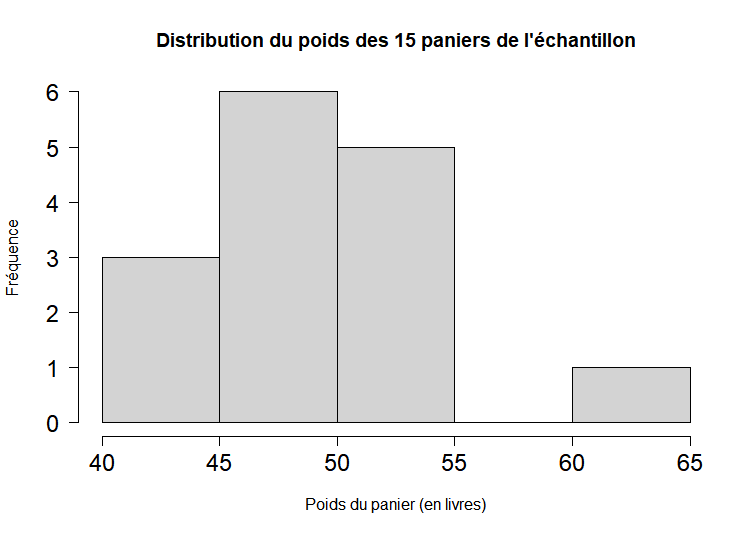
\includegraphics[scale=0.5]{HistPommes.png}
\end{center}

Utilisez le graphique ci-dessus pour estimer le poids moyen des 15 paniers de son échantillon. Laissez des traces de votre démarche.

\begin{solution}
On calcule $(1/15) * ( 42,5 *3 + 47,5*6 + 52,5 *5 + 57,5*0 + 62,5*1) = 737.5/15 = 49,1666$
\end{solution}

\end{parts}
\end{A22}

\begin{H23}
\question (H23) \label{H23-I11-micro}
Dans un laboratoire de microtechnique, un technicien a étudié le temps de réaction (en millisecondes) d'un certain type de détecteur de mouvements. Les 21 valeurs suivantes sont des temps de réaction collectés au cours d'une journée par ordre croissant:

\begin{center}
\begin{tabular}{  c c c c c c c c }
111  &111  &111  &112  &113  &113  &113 \\
113 &114  &114  &114  &114 &115 & 116 \\
118 & 118 & 118 & 119 & 125 &127 & 128\\
\end{tabular}
\end{center}

Le diagramme en boîte ci-dessous a été tracé à partir de ces résultats. Il manque toutefois quelque chose à ce diagramme (il ne s'agit pas d'un titre ou de noms d'axes).

\medskip

\begin{parts}
\part[6] Ajoutez \textbf{sur le diagramme} l'élément manquant et dites ce que vous avez fait (ceci \textit{doit} inclure des calculs) sous le diagramme.
\begin{solution}
L'élément manquant est la ligne de la \textbf{médiane} à l'intérieur de la boîte.

Avec $n=21$ observations, la médiane est la $\frac{21+1}{2} = 11$\textsuperscript{e} observation, soit $\tilde{x} = 114$.

On trace donc un trait vertical à $x = 114$ à l'intérieur de la boîte.
\end{solution}
\begin{center}
		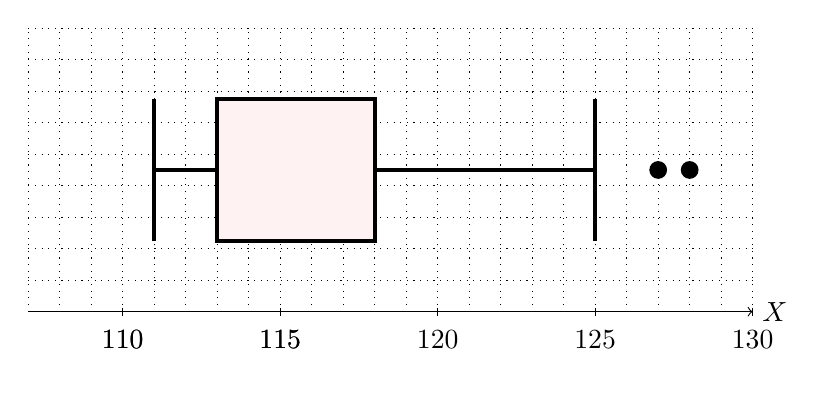
\begin{tikzpicture}[x=0.4cm,y=0.9cm]
         \draw[step=0.4cm,,dotted,color=black] (107,0) grid (130,4);
		\draw[->] (107,0) -- (130,0) node[right] {$X$} ;
		\foreach \X in {110,115,110,115,120,125,130} {
			\draw (\X,0.05cm) -- (\X,-0.05cm) node[below] {$\X\strut$};}
		\draw[ultra thick][fill=red!5] (113,1) rectangle (118,3);
		\draw[ultra thick] (111,1) -- (111,3);
		\draw[ultra thick] (111,2) -- (113,2);
		\draw[ultra thick] (118,2) -- (125,2);
		
		\draw[ultra thick] (125,1) -- (125,3);
        \filldraw [black] (127, 2) circle (3pt);
        \filldraw [black] (128, 2) circle (3pt);
			\end{tikzpicture}\\
	\end{center}

\pagesuivante{\ref{H23-I11-micro}}

\suite{\ref{H23-I11-micro}}

\part Vous apprenez que la plus grande observation (128) est erronée. Vous ne connaissez pas sa valeur, mais vous savez que celle-ci est plus grande que 150. Nous notons cette valeur XXX et nous savons que XXX~>~150. Le nouveau jeu de données est donc:

\begin{center}
\begin{tabular}{  c c c c c c c c }
111  &111  &111  &112  &113  &113  &113 \\
113 &114  &114  &114  &114 &115 & 116 \\
118 & 118 & 118 & 119 & 125 &127 & XXX \\
\end{tabular}
\end{center}

À partir de ce nouveau jeu de données, répondez aux questions suivantes. Nous nommons «jeu de données original» celui qui contient l'observation 128 et «nouveau jeu de données» celui qui contient l'observation XXX.

\textbf{\textit{Inscrivez «Vrai» ou «Faux» dans les cases appropriées.}}

\begin{subparts}
\subpart[3]La médiane échantillonnale du nouveau jeu de données est supérieure à celle du jeu de données orginal.

    \begin{oneparcheckboxes}
        \choice Vrai
        \correctchoice Faux
    \end{oneparcheckboxes}
\begin{solution}
La médiane est la 11\textsuperscript{e} observation ($n=21$), soit $\tilde{x}=114$ dans les deux cas. Remplacer la 21\textsuperscript{e} observation ne change pas la 11\textsuperscript{e}. Les médianes sont égales.
\end{solution}

\subpart[3] La moyenne échantillonnale du nouveau jeu de données est supérieure à celle du jeu de données original.

    \begin{oneparcheckboxes}
        \correctchoice Vrai
        \choice Faux
    \end{oneparcheckboxes}
\begin{solution}
On remplace 128 par $\text{XXX} > 150$. La somme augmente, donc $\bar{x}$ augmente aussi.
\end{solution}

\subpart[3] La variance échantillonnale du nouveau jeu de données est supérieure à celle du jeu de données orignal.

    \begin{oneparcheckboxes}
        \correctchoice Vrai
        \choice Faux
    \end{oneparcheckboxes}
\begin{solution}
La nouvelle observation est plus éloignée de la moyenne que l'ancienne (128), ce qui augmente la somme des écarts au carré et donc la variance.
\end{solution}

\end{subparts}
\end{parts}
\end{H23}

\begin{A23}
\question (A23) \label{A23-I11-micro}
Dans un laboratoire de microtechnique, Audrey et Vincent ont étudié le temps de réaction (en millisecondes) d'un certain type de détecteur de mouvements. Les 21 valeurs suivantes sont des temps de réaction collectés au cours d'une journée:

\begin{center}
\begin{tabular}{  c c c c c c c c }
111  &111  &111  &112  &113  &113  &113 \\
113 &115  &115  &115  &115 &115 & 116 \\
116 & 118 & 118 & 119 & 125 &125 & 128\\
\end{tabular}
\end{center}

Le diagramme en boîte ci-dessous a été tracé à partir de ces résultats. Il manque toutefois quelque chose à ce diagramme (il ne s'agit pas d'un titre ou de noms d'axes).

\medskip

\begin{parts}
\part[3] Ajoutez \textbf{sur le diagramme} l'élément manquant et dites ce que vous avez fait (ceci \textit{doit} inclure des calculs) sous le diagramme. Un ajout sur le diagramme sans justification n'aura aucun point.
\begin{center}
		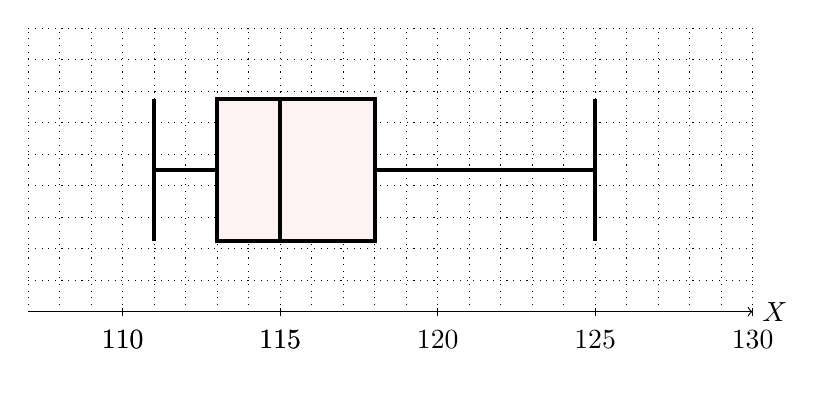
\begin{tikzpicture}[x=0.4cm,y=0.9cm]
         \draw[step=0.4cm,,dotted,color=black] (107,0) grid (130,4);
		\draw[->] (107,0) -- (130,0) node[right] {$X$} ;
		\foreach \X in {110,115,110,115,120,125,130} {
			\draw (\X,0.05cm) -- (\X,-0.05cm) node[below] {$\X\strut$};}
		\draw[ultra thick][fill=red!5] (113,1) rectangle (118,3);
  	\draw[ultra thick] (115,1) -- (115,3);

		\draw[ultra thick] (111,1) -- (111,3);
		\draw[ultra thick] (111,2) -- (113,2);
		\draw[ultra thick] (118,2) -- (125,2);
		
		\draw[ultra thick] (125,1) -- (125,3);
			\end{tikzpicture}\\
	\end{center}
 \begin{solution}
     Il manque la médiane à (114 + 114) /2 = 114
 \end{solution}

\pagesuivante{\ref{A23-I11-micro}}
 . 
\suite{\ref{A23-I11-micro}}

\part[6] Nous apprenons que la plus grande observation (128) est erronée. Nous ne connaissons pas sa valeur, mais nous savons que celle-ci est plus grande que 150. Nous notons cette valeur XXX et nous savons que XXX~$>$~150. Le nouveau jeu de données est donc:

\begin{center}
\begin{tabular}{  c c c c c c c c }
111  &111  &111  &112  &113  &113  &113 \\
113 &115  &115  &115  &115 &115 & 116 \\
116 & 118 & 118 & 119 & 125 &127 & XXX\\
\end{tabular}
\end{center}

À partir de ce nouveau jeu de données, répondez aux questions suivantes. Nous nommons «jeu de données original» celui qui contient l'observation 128 et «nouveau jeu de données» celui qui contient l'observation XXX.

Déterminez si les énoncés suivants sont vrais ou faux. 

\textbf{\textit{Une bonne réponse vaut 2 points, une mauvaise réponse vaut -1 point et une réponse vide vaut 0 point, pour un total minimum de 0 point.}}

\begin{subparts}
\subpart La médiane échantillonnale du nouveau jeu de données est supérieure à celle du jeu de données original.

    \begin{oneparcheckboxes}
        \choice Vrai
        \correctchoice Faux
    \end{oneparcheckboxes}
    
\begin{solution}
    Faux
\end{solution}

\subpart La moyenne échantillonnale du nouveau jeu de données est supérieure à celle du jeu de données original.

    \begin{oneparcheckboxes}
        \correctchoice Vrai
        \choice Faux
    \end{oneparcheckboxes}
    
\begin{solution}
    Vrai
\end{solution}

\subpart La variance échantillonnale du nouveau jeu de données est supérieure à celle du jeu de données original.

    \begin{oneparcheckboxes}
        \correctchoice Vrai
        \choice Faux
    \end{oneparcheckboxes}
    
\begin{solution}
    Vrai
\end{solution}

\end{subparts}
\end{parts}

 .
\end{A23}

\begin{A23}
\question (A23) 
Parmi les statistiques descriptives suivantes, lesquelles sont des mesures de dispersion? \textit{\textbf{Une réponse cochée alors qu'elle ne devrait pas l'être entraîne une pénalité de 1 points. Le minimum possible pour cette question est 0 point.}}

\begin{checkboxes}
\choice La moyenne échantillonnale
\choice La médiane échantillonnale
\choice Le mode échantillonnal
\correctchoice La variance échantillonnale
\correctchoice L'écart interquartile
\correctchoice L'étendue
\end{checkboxes}
\end{A23}

\begin{A24}
\question (A24) Soit le jeu de données $x_1,\hdots,x_n$, où $n$ est une nombre impair. Nous supposons que toutes les valeurs sont différentes. La moyenne échantillonnale de ce jeu de données est $\overline{x}$ et sa médiane est $\widetilde{x}$.

Dans chacune des situations suivantes, cochez toutes les réponses vraies.
\begin{parts}
    \part[2] Que pouvons-nous faire pour augmenter $\overline{x}$ sans augmenter $\widetilde{x}$?
    \begin{checkboxes}
        \choice Changer la valeur de $x_{(1)}$ pour une valeur supérieure à $x_{(n)}$
        \choice Changer la valeur de $x_{(n)}$ pour une valeur inférieure à $x_{(1)}$
        \correctchoice Changer la valeur de $x_{(n)}$ pour une valeur supérieure à $x_{(n)}$
        \correctchoice Changer la valeur de $x_{(1)}$ pour une valeur supérieure à $x_{(1)}$, mais inférieure à $\displaystyle x_{(0,5n + 0,5)}$
    \end{checkboxes}

    \part[2] Que pouvons-nous faire pour augmenter $\overline{x}$ et $\widetilde{x}$?
    \begin{checkboxes}
        \choice Changer la valeur de $x_{(1)}$ pour une valeur supérieure à $x_{(n)}$
        \choice Changer la valeur de $x_{(n)}$ pour une valeur inférieure à $x_{(1)}$
        \correctchoice Changer la valeur de $x_{(n)}$ pour une valeur supérieure à $x_{(n)}$
        \correctchoice Changer la valeur de $x_{(1)}$ pour une valeur supérieure à $x_{(1)}$, mais inférieure à $\displaystyle x_{(0,5n + 0,5)}$
    \end{checkboxes}
\end{parts}
\end{A24}

\begin{A24}
\question (A24) \label{A24-F8-micro}
Soit les 21 valeurs suivantes:

\begin{center}
\begin{tabular}{  c c c c c c c c }
111  &112  &112  &112  &113  &113  &113 \\
113 &115  &115  &115  &115 &115 & 116 \\
118 & 118 & 118 & 119 & 124 &124 & 125\\
\end{tabular}
\end{center}

Le diagramme en boîte ci-dessous a été tracé à partir de ces résultats. Il y a toutefois au moins une erreur (il ne s'agit pas d'un titre ou de noms d'axes).

\begin{center}
		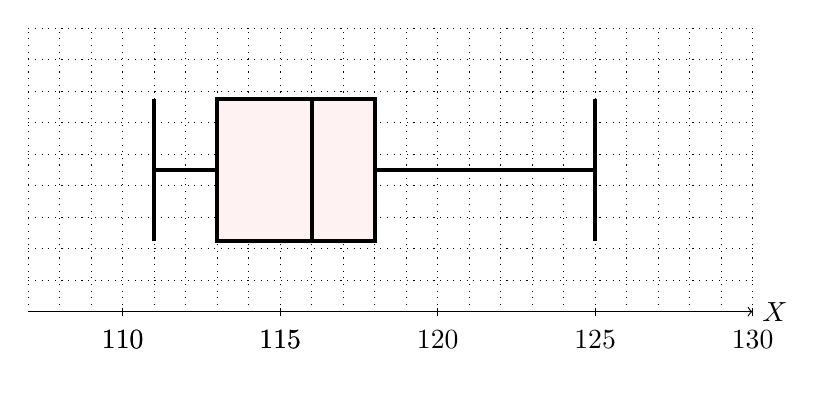
\begin{tikzpicture}[x=0.4cm,y=0.9cm]
         \draw[step=0.4cm,,dotted,color=black] (107,0) grid (130,4);
		\draw[->] (107,0) -- (130,0) node[right] {$X$} ;
		\foreach \X in {110,115,110,115,120,125,130} {
			\draw (\X,0.05cm) -- (\X,-0.05cm) node[below] {$\X\strut$};}
		\draw[ultra thick][fill=red!5] (113,1) rectangle (118,3);
  	\draw[ultra thick] (116,1) -- (116,3);

		\draw[ultra thick] (111,1) -- (111,3);
		\draw[ultra thick] (111,2) -- (113,2);
		\draw[ultra thick] (118,2) -- (125,2);
		
		\draw[ultra thick] (125,1) -- (125,3);

			\end{tikzpicture}\\
	\end{center}

Quelle est cette erreur?

  \begin{checkboxes}
\choice La médiane n'est pas au bon endroit.  
\choice La moyenne échantillonnale n'est pas au bon endroit. 
\choice Il devrait y avoir deux points: un à 105,5 et un à 125,5.
\choice La moustache de gauche devrait être à  105,5. 
\choice La moustache de droite devrait être à 125,5.
\choice Il n'y a aucune erreur.
\end{checkboxes}

.
\end{A24}

\begin{A25}
\question (A25) Soit l'histogramme suivant:

\begin{center}
    
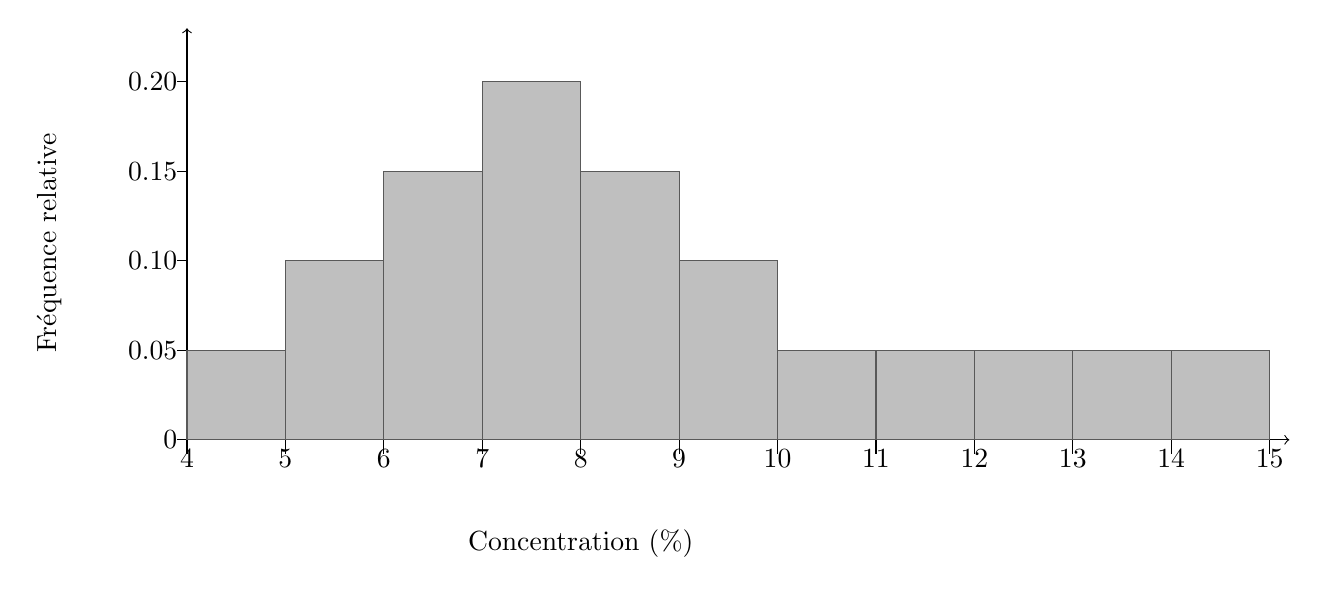
\begin{tikzpicture}[x=1.25cm, y=22.727cm] 
  
  \draw[->] (4,0) -- (15.2,0);
  \draw[->] (4,0) -- (4,0.23);

  
  \foreach \x in {4,...,15} {
    \draw (\x,0) -- (\x,-0.008);
    \node[below] at (\x,0) {\x};
  }

  
  \foreach \y/\lab in {0/0,0.05/0.05,0.10/0.10,0.15/0.15,0.20/0.20}{
    \draw (4,\y) -- (3.9,\y);
    \node[left] at (4,\y) {\lab};
  }

  
  \node[below] at (8,-0.045) {Concentration (\%)};
  \node[rotate=90] at (2.6,0.11) {Fréquence relative};

  
  \foreach \x/\h in {4/0.05,5/0.1,6/0.15,7/0.20,8/0.15,9/0.1,10/0.05,11/0.05,12/0.05,13/0.05,14/0.05} {
    \fill[gray!50] (\x,0) rectangle (\x+1,\h);
    \draw[gray!70!black] (\x,0) rectangle (\x+1,\h);
  }
\end{tikzpicture}
\end{center}

Déterminez si les énoncés suivants sont vrais ou faux. 

\textbf{\textit{Une bonne réponse vaut 1 points, une mauvaise réponse vaut -1 point et une réponse vide vaut 0 point, pour un total minimum de 0 point.}}

\begin{parts}
    \part[2] Il est impossible de donner la taille de l'échantillon qui a servi à tracer cet histogramme avec l'information donnée.

    \begin{oneparcheckboxes}
        \correctchoice Vrai
        \choice Faux
    \end{oneparcheckboxes}

\part[2] Cet histogramme est typique de données provenant d'une distribution où la moyenne est supérieure à la médiane.

    \begin{oneparcheckboxes}
        \correctchoice Vrai
        \choice Faux
    \end{oneparcheckboxes}

\part[2] L'écart interquartile vaut au moins 5,5.

    \begin{oneparcheckboxes}
        \choice Vrai
        \correctchoice Faux
    \end{oneparcheckboxes}

    

\part[2] La médiane échantillonnale est entre 7\% et 9\%, inclusivement.

    \begin{oneparcheckboxes}
        \correctchoice Vrai
        \choice Faux
    \end{oneparcheckboxes}

\part[2] L'écart-type échantillonnal est de 11\%.

    \begin{oneparcheckboxes}
        \choice Vrai
        \correctchoice Faux
    \end{oneparcheckboxes}
    
    \end{parts}
\end{A25}

\begin{H26}
\question (H26) Dites si les énoncés suivants sont vrais ou faux.

\begin{parts}
    \part[1] Soit $x_1,\hdots,x_n$. Si la médiane échantillonnale est $25$, nous sommes certains que la valeur de l'observation du milieu est $25$.

    \begin{oneparcheckboxes}
        \choice Vrai
        \correctchoice Faux
    \end{oneparcheckboxes}

    \begin{solution}
    Faux. Si $n$ est pair, la médiane est la moyenne des deux observations centrales; aucune d'elles n'est forcément égale à $25$. Cette propriété n'est garantie que si $n$ est impair.
    \end{solution}

        \part[1] Soit $x_1,\hdots,x_n$. Si la moyenne échantillonnale est $25$, environ $50\%$ des observations sont plus grandes que $25$ et environ $50\%$ sont plus petites que $25$.

    \begin{oneparcheckboxes}
        \choice Vrai
        \correctchoice Faux
    \end{oneparcheckboxes}
    
    \begin{solution}
    Faux. C'est une propriété de la \textbf{médiane}, pas de la moyenne. La moyenne est sensible aux valeurs extrêmes et ne partage pas nécessairement l'échantillon en deux moitiés égales.
    \end{solution}

        \part[1] Soit $x_1,\hdots,x_n$. Si $Q_1=12$, nous savons que le minimum de l'échantillon est 12.

    \begin{oneparcheckboxes}
        \choice Vrai
        \correctchoice Faux
    \end{oneparcheckboxes}
 
    \begin{solution}
    Faux. $Q_1$ est le premier quartile (25\textsuperscript{e} percentile); le minimum de l'échantillon peut être strictement inférieur à $Q_1$.
    \end{solution}

        \part[1] Soit $x_1,\hdots,x_n$. Nous savons que $Q_3>0$.

    \begin{oneparcheckboxes}
        \choice Vrai
        \correctchoice Faux
    \end{oneparcheckboxes}

    \begin{solution}
    Faux. $Q_3$ dépend des données. Si toutes les observations sont négatives, $Q_3<0$.
    \end{solution}
    

\end{parts}
\end{H26}

\begin{H26}
\question (H26) 
\noindent
\begin{minipage}[t]{0.5\linewidth}
Soit l'histogramme ci-contre.

Dans quelle classe de l'histogramme se situe le quantile d'ordre 0,30?

\begin{checkboxes}
  \choice Dans la classe [10,15[
  \correctchoice Dans la classe [15,20[
  \choice Dans la classe [20,25[
  \choice Dans la classe [25,30[
  \choice Dans la classe [30,35[
\end{checkboxes}
\end{minipage}\hfill
\begin{minipage}[t]{0.42\linewidth}
\centering
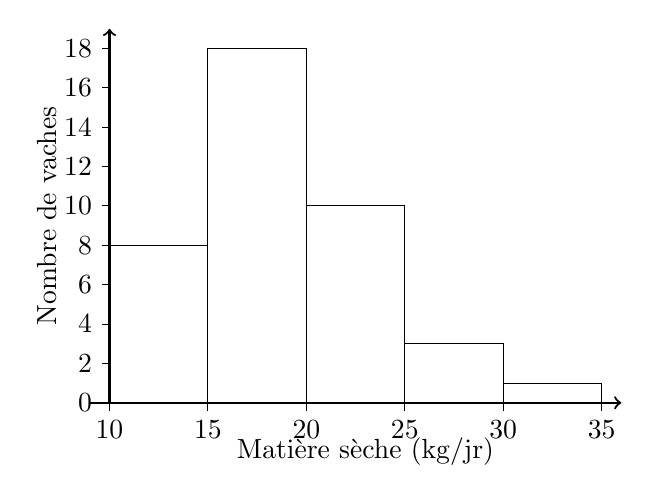
\begin{tikzpicture}[x=0.25cm,y=0.25cm]

\draw[->, thick] (9,0) -- (36,0);   
\draw[->, thick] (10,0) -- (10,19); 

\foreach \x in {10,15,20,25,30,35}
  \draw (\x,0) -- (\x,-0.4) node[below] {\x};

\foreach \y in {0,2,4,6,8,10,12,14,16,18}
  \draw (10,\y) -- (9.6,\y) node[left] {\y};

\node at (23,-2.5) {Mati\`ere s\`eche (kg/jr)};
\node[rotate=90] at (6.8,9.5) {Nombre de vaches};

\draw (10,0) rectangle (15,8);
\draw (15,0) rectangle (20,18);
\draw (20,0) rectangle (25,10);
\draw (25,0) rectangle (30,3);
\draw (30,0) rectangle (35,1);

\end{tikzpicture}
\end{minipage}

\begin{solution}
    Le nombre total de vaches est $8+18+10+3+1=40$. Le quantile d'ordre $0{,}30$ correspond à la position $0{,}30 \times 40 = 12$. L'effectif cumulé après la classe $[10,15[$ est $8$. L'effectif cumulé après la classe $[15,20[$ est $8+18=26$. Puisque $8 < 12 \leq 26$, le quantile d'ordre $0{,}30$ se situe dans la classe $[15,20[$.
\end{solution}
\end{H26}

\begin{H26}
\question (H26) 
Dans un laboratoire de microtechnique, Benjamin et Guillaume ont étudié le temps de réaction (en millisecondes) d'un certain type de détecteur de mouvements. Les 21 valeurs suivantes sont des temps de réaction collectés au cours d'une journée:

\begin{center}
\begin{tabular}{  c c c c c c c c }
111  &111  &111  &112  &113  &113  &113 \\
113 &115  &115  &115  &115 &115 & 116 \\
116 & 118 & 118 & 119 & 125 &125 & 128\\
\end{tabular}
\end{center}

Le diagramme en boîte ci-dessous a été tracé à partir de ces résultats. Il manque toutefois quelque chose à ce diagramme (il ne s'agit pas d'un titre ou de noms d'axes).

Ajoutez \textbf{sur le diagramme} l'élément manquant et dites ce que vous avez fait sous le diagramme. 
\begin{center}
		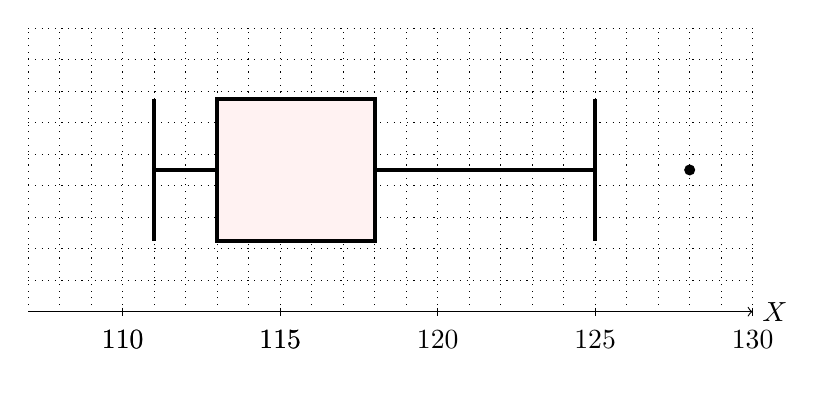
\begin{tikzpicture}[x=0.4cm,y=0.9cm]
         \draw[step=0.4cm,,dotted,color=black] (107,0) grid (130,4);
		\draw[->] (107,0) -- (130,0) node[right] {$X$} ;
		\foreach \X in {110,115,110,115,120,125,130} {
			\draw (\X,0.05cm) -- (\X,-0.05cm) node[below] {$\X\strut$};}
		\draw[ultra thick][fill=red!5] (113,1) rectangle (118,3);

		\draw[ultra thick] (111,1) -- (111,3);
		\draw[ultra thick] (111,2) -- (113,2);
        
		\draw[ultra thick] (118,2) -- (125,2);
		
		\draw[ultra thick] (125,1) -- (125,3);
        \node[circle, fill=black, inner sep=0pt, minimum size=4pt] at (128,2) {};
			\end{tikzpicture}\\
	\end{center}

\begin{solution}
    Il manque la ligne de la médiane dans le diagramme en boîte. Les 21 données ordonnées donnent une médiane égale à la 11\textsuperscript{e} valeur, soit $\tilde{x}=115$. Il faut donc tracer un trait vertical à $x=115$ à l'intérieur de la boîte.

    On vérifie les autres éléments:
    \begin{itemize}
        \item $Q_1 = (x_{(5)}+x_{(6)})/2=(113+113)/2=113$ \checkmark
        \item $Q_3 = (x_{(16)}+x_{(17)})/2=(118+118)/2=118$ \checkmark
        \item $\text{IQR}=Q_3 - Q_1 = 5$
        \item Barrière supérieure: $Q_3+1{,}5\times\text{IQR}=118+7{,}5=125{,}5$
        \item La valeur $128 > 125{,}5$ est une valeur aberrante, correctement représentée par un point. \checkmark
        \item La moustache supérieure s'arrête à $125$, la plus grande valeur non aberrante. \checkmark
        \item La moustache inférieure s'arrête à $111$, la plus petite valeur. \checkmark
    \end{itemize}
\end{solution}
\end{H26}

\begin{H26r}
\question (H26r) Dites si les énoncés suivants sont vrais ou faux. Aucune justification n'est requise.

\begin{parts}

    \part[1] Soit $x_1,\ldots,x_n$. Si la médiane vaut $25$, environ $50\%$ des observations sont supérieures à $25$ et environ $50\%$ sont inférieures à $25$.

    \begin{oneparcheckboxes}
        \correctchoice Vrai
        \choice Faux
    \end{oneparcheckboxes}

    \begin{solution}
    Vrai. C'est la définition de la médiane : elle partage l'échantillon en deux moitiés égales.
    \end{solution}

    \part[1] Soit $x_1,\ldots,x_n$. Si on ajoute une constante $c>0$ à chaque observation, l'écart-type ne change pas.

    \begin{oneparcheckboxes}
        \correctchoice Vrai
        \choice Faux
    \end{oneparcheckboxes}

    \begin{solution}
    Vrai. L'écart-type mesure la dispersion autour de la moyenne. Une translation de toutes les observations ne modifie pas les distances entre les valeurs et leur moyenne.
    \end{solution}

    \part[1] Soit $x_1,\ldots,x_n$. L'étendue est une mesure de dispersion résistante à la présence de valeurs aberrantes.

    \begin{oneparcheckboxes}
        \choice Vrai
        \correctchoice Faux
    \end{oneparcheckboxes}

    \begin{solution}
    Faux. L'étendue est définie comme la différence entre le maximum et le minimum, et est donc très sensible aux valeurs extrêmes.
    \end{solution}

    \part[1] Soit $x_1,\ldots,x_n$. Si la variance échantillonnale $S^2$ vaut $0$, alors toutes les observations sont identiques.

    \begin{oneparcheckboxes}
        \correctchoice Vrai
        \choice Faux
    \end{oneparcheckboxes}

    \begin{solution}
    Vrai. $S^2=0$ implique que chaque terme $(X_i-\overline{X})^2=0$, donc $X_i=\overline{X}$ pour tout $i$.
    \end{solution}

\end{parts}
\end{H26r}

\begin{H26r}
\question (H26r) 

Supposons le petit échantillon suivant :
\[
2,\;4,\;4,\;6,\;9.
\]

Ajoutez une observation à ce jeu de données de façon à diminuer la moyenne sans modifier la médiane. Justifiez brièvement votre réponse.

\begin{solution}
Une réponse possible est d'ajouter \(1\).

Le nouveau jeu de données ordonné est
\[
1,\;2,\;4,\;4,\;6,\;9.
\]

La médiane reste égale à
\[
\frac{4+4}{2}=4.
\]

La moyenne initiale est
\[
\bar{x}=\frac{2+4+4+6+9}{5}=5.
\]

La nouvelle moyenne est
\[
\bar{x}_{\text{nouvelle}}=\frac{1+2+4+4+6+9}{6}
=
\frac{26}{6}
\approx 4{,}33.
\]

La moyenne a donc diminué.
\end{solution}
\end{H26r}

\begin{H26r}
\question (H26r) 

Vous voulez connaître l'âge des gens présents à une fête de quartier. Un ami questionne tous les individus présents et vous remet les résultats sous la forme suivante: 

\begin{table}[h!]
\begin{center}
\begin{tabular}{c|c}
Classe d'âge & Fréquence \\
\hline
$[0,5]$ & 8 \\
$[5,10]$ & 15 \\
$[10, 25]$ & 6 \\
$[25, 40]$ & ? \\
$[40, 100]$ & 10 
\end{tabular}
\end{center}
\end{table}

Le nombre d'individus âgés entre 25 et 40 ans est illisible. Votre ami avait toutefois pris le temps de faire un histogramme des données et vous informe que la hauteur du rectangle pour le groupe des individus âgés de 5 à 10 ans est de 0,06. Déduisez le nombre total de personnes présentes à la fête de quartier. 

\begin{solution}
Dans un histogramme, la hauteur $h$ d'une classe est donnée par: 
\begin{align*}
h=\frac{\mbox{Fréquence relative}}{\mbox{longueur de la classe}}
\end{align*}
donc
\begin{align*}
\mbox{Fréquence relative}=hauteur\times\mbox{longueur de la classe}=0.06\times(10-5)=0.3
\end{align*}
Aussi, la fréquence relative est donnée par: 
\begin{align*}
\mbox{Fréquence relative}=\frac{\mbox{Fréquence}}{\mbox{nombre total d'observations}}
\end{align*}
On déduit donc que: 
\begin{align*}
\mbox{nombre total d'observations} =\frac{\mbox{Fréquence}}{\mbox{Fréquence relative}}=\frac{15}{0.3}=50
\end{align*}
Le nombre total de personnes présentes à la fête de quartier est donc de $n=50$.    
\end{solution}
\end{H26r}


\moduleheader{mod7}{Module 7 - Estimation et intervalles de confiance}

\begin{A22}
\question (A22)  
Jean-Claude suppose que le temps d'attente à l'hôpital suit une exponentielle de moyenne 240 minutes. 
Il veut construire un intervalle de confiance bilatéral à $95\%$ pour le vérifier.
Il procède donc comme suit. 
Il veut prend le temps d'attente de $16$ personnes choisies au hasard et connaître $\Bar{X}$ et $S^2$. 
Il obtient $\Bar{x}=250$ et $s^2=59'536$.
Comme il construit un intervalle de confiance bilatéral, il choisit $z_{\alpha/2}=1,96$, à partir de sa table de la loi normale.
Son intervalle de confiance à $95\%$ est donc $[130,44;369,56]$.
Comme celui-ci contient $240$, il se dit que cette valeur est plausible pour $\mu$. 
Après avoir vérifié les résultats de Jean-Claude, vous constatez qu'il y a une erreur dans ce qu'il a fait. 
Quelle est cette erreur?

\begin{solution}
   Comme $n=16<30$, on ne peut pas utiliser le TCL.
\end{solution}
\end{A22}

\begin{A22}
\question (A22) 
Si $X \sim \chi^2_{24}$, alors $P(X<0)=P(X>0)=0.5$.

\begin{oneparcheckboxes}
\choice Vrai
\choice Faux
\end{oneparcheckboxes}
\end{A22}

\begin{A22}
\question (A22) 
Sachant que $\displaystyle \frac{(n-1)S^2}{\sigma^2}$ suit une loi du khi-carré à $n-1$ degrés de liberté, donnez $\text{Var}(S^2)$.

\begin{solution}
On peut calculer que 
\begin{align*}
Var(S^2) &= Var\left( \frac{\sigma^2}{(n-1)}\frac{(n-1)}{\sigma^2}S^2 \right)\\
    &= \frac{\sigma^4}{(n-1)^2} Var\left(\frac{(n-1)}{\sigma^2}S^2\right)  \\
    &= \frac{\sigma^4}{(n-1)^2}(2(n-1)) \\
    &= \frac{2\sigma^4}{(n-1)}
\end{align*}
\end{solution}
\end{A22}

\begin{A22}
\question (A22) 

On a construit un intervalle de confiance pour la proportion de personnes qui préfèrent le chocolat noir au chocolat au lait. On a utilisé un échantillon de $2400$ personnes, parmi lesquelles $960$ ont répondu qu’elles préféraient le chocolat noir. On a obtenu l’intervalle $[37, 83\%; 42, 17\%]$. Quel est le niveau de confiance de cet intervalle ?

\begin{solution}
La marge d'erreur de l'intervalle est 
$$ \frac{42,17-37,82}{2} = 2,175\%$$ 
On a donc 
\begin{align*}
0,02175 &= z_{\alpha/2}\sqrt{\frac{\hat{p}{(1-\hat{p}}}{n}} \\ 
&= z_{\alpha/2} \sqrt{\frac{960/2400{(1-960/2400)}}{2400}}\\
&= z_{\alpha/2} 0,01
\end{align*}
On trouve donc que $z_{\alpha/2} = 2,175$. La table nous indique que $\alpha/2 = 1-0.985 = 0.015$ et donc que $\alpha = 0.03$. Le niveau de confiance de l'intervalle est donc $0.97$. 
\end{solution}
\end{A22}

\begin{A22}
\question (A22) 

On s'intéresse aux frais d'inscriptions des étudiants de 1er cycle à temps plein au Québec. 
Avec un échantillon aléatoire de $n=121$ étudiants de la population, on obtient l'intervalle de confiance à 95\% suivant: $[2\,550;2\,630]$. 
Cochez tous les énoncés qui sont vrais parmi les suivants. (Aucune justification requise)

\begin{checkboxes}
\choice Il y a 95\% des étudiants de 1er cycle à temps plein au Québec qui paient des frais d'inscription entre 2\,550 \$ et 2\,630 \$
\choice Si on pigeait un échantillon de 1\,000 étudiants pour construire un nouvel intervalle de confiance à 95\% sur la moyenne, celui-ci aurait une plus grande probabilité de contenir la vraie valeur de $\mu$ que celui obtenu à partir de 121 étudiants.
\choice Si on pigeait un autre échantillon de 121 étudiants pour construire un intervalle de confiance à 95\% sur la moyenne, l'intervalle obtenu aurait la même longueur que celui-ci.
\choice Si on pigeait plusieurs échantillons de 121 étudiants dans cette population, et qu'on construisait avec chacun d'eux l'intervalle de confiance à 95\% pour $\mu$, alors environ 95\% de ces intervalles contiendraient la vraie valeur moyenne des frais d'inscription des étudiants de 1er cycle à temps plein au Québec. 
\end{checkboxes}

\begin{solution}
Seul le dernier énoncé est vrai. 
\end{solution}
\end{A22}

\begin{A22}
\question (A22) 
On souhaite effectuer une étude afin de savoir ce que les gens préfèrent entre la fondue et la raclette. Pour cette étude, on supposera que les réponses des gens $X_1,\hdots,X_n$ sont indépendantes et identiquement distribuées selon une Bernoulli($p$), où $p$ représente la probabilité de choisir la fondue. Quelle doit être la taille d'échantillon minimale si on désire que notre intervalle de confiance à 90\% pour $p$ ait une longueur maximale de $0,04$?
\begin{solution}
    fff
\end{solution}
\end{A22}

\begin{A22}
\question (A22) On suppose deux populations distribuées selon des lois normales de moyennes $\mu_1$ et $\mu_2$ et de variances $\sigma^2_1$ et $\sigma^2_2$ inconnues qui sont supposées égales. Vous avez les échantillons

\begin{align*}
X_{11}, \ldots, X_{1n_1} \overset{i.i.d.}{\sim} N(\mu_1, \sigma^2_1), & & X_{21}, \ldots, X_{2n_2} \overset{i.i.d.}{\sim} N(\mu_2, \sigma^2_2),
\end{align*}
où $n_1=8$ et $n_2=8$. Vous avez construit un intervalle de confiance à $95\%$ pour $\mu_1-\mu_2$ et obtenu $[0,1; 4,39]$. Lors de la présentation des résultats, vous réalisez que vous avez pris en note que $S^2_1=4,52$, mais vous ne trouvez plus la valeur de $S^2_2$. 
\begin{parts}
    \part[8] Quelle est la valeur de $S^2_2$?
    
    \part[2] Que pouvez-vous dire au sujet de $\mu_1-\mu_2$?
\end{parts}

\begin{solution}
    
\end{solution}
\end{A22}

\begin{A22}
\question (A22) Clara se déplace en autobus pour aller travailler et elle note minutieusement le temps nécessaire pour ses déplacements. Voici ses cinq derniers temps de déplacements, en minutes : 
$$ 22, 25, 24, 21, 33.$$
On peut supposer que ses temps de déplacements sont indépendants et suivent une loi normale de moyenne $\mu$ et de variance $\sigma^2$.

\begin{parts}
\part[6]

Donnez un intervalle de confiance à 90\% pour la variance de ses temps de déplacement.
\begin{solution}
On doit d'abord calculer la variance échantillonnale. On trouve 
$$\bar{x} = \frac{1}{5}(22+25+24+21+33) = 25$$
On a ensuite 
\begin{align*}
s^2 &= \frac{1}{4}\left( (22-25)^2 + (25-25)^2 + (24-25)^2 + (21-25)^2 + (33-25)^2 \right)\\
&= \frac{1}{4}(9+0+1+16+64) \\
&= \frac{90}{4}\\
&= 22,5 \mbox{ minutes}^2    
\end{align*}  

Puisque $\alpha = 0.1$ on doit chercher dans la table $\chi^2_{0.05,4} = 9,49$ et $\chi^2_{0.95,4} = 0,71$. 
Notre intervalle est donc 
$$ \left[ \frac{4*22,5}{9,49} = 9,48, \frac{4*22,5}{0.71} =126,76 \right] $$
\end{solution}

\part[2] 
Est-ce une bonne idée d'utiliser le point milieu de cet intervalle comme estimateur ponctuel pour $\sigma^2$? Justifiez votre réponse.

\begin{solution}
Non. On sait que $s^2$ est non biaisé pour $\sigma^2$ et le centre de l'IC n'est pas $s^2$.
\end{solution}

\part[2]
Un collègue vous fait remarquer que la taille d'échantillon est très petite et que votre intervalle de confiance n'est probablement pas valide. Que lui répondez-vous?
\begin{solution}
Si les données suivent bien une loi normale, cet IC est valide peu importe la taille d'échantillon.
\end{solution}

\end{parts}
\end{A22}

\begin{H23}
\question (H23) \label{H23-F1-QCMicTests}
Un intervalle de confiance de niveau 95\% pour la moyenne théorique $\mu$ est $[ 5,11 ; 9,11]$. Pour chaque énoncé qui suit, indiquez si l'énoncé est vrai, faux ou si nous n'avons pas assez d'information pour le savoir.

\medskip

\begin{parts}
    \part[1] Au seuil 5\%, on rejette $H_0: \mu=5$ pour $H_1:\mu \neq 5$.

\medskip
    \begin{oneparcheckboxes}
        \CorrectChoice Vrai 
        \choice Faux
        \choice Nous n'avons pas assez d'information pour le savoir.
    \end{oneparcheckboxes}
\medskip
 
   \part[1] Au seuil 1\%, on rejette $H_0: \mu=5$ pour $H_1:\mu \neq 5$.

 \medskip  \begin{oneparcheckboxes}
        \choice Vrai 
        \choice Faux
        \CorrectChoice Nous n'avons pas assez d'information pour le savoir.
\medskip    \end{oneparcheckboxes}
    
   \part[1] Au seuil 10\%, on rejette $H_0: \mu=5$ pour $H_1:\mu \neq 5$.

\medskip   \begin{oneparcheckboxes}
        \CorrectChoice Vrai 
        \choice Faux
        \choice Nous n'avons pas assez d'information pour le savoir.
\medskip    \end{oneparcheckboxes}
    
   \part[1] Au seuil 5\%, on rejette $H_0: \mu=8$ pour $H_1:\mu \neq 8$.

\medskip   \begin{oneparcheckboxes}
        \choice Vrai 
        \CorrectChoice Faux
        \choice Nous n'avons pas assez d'information pour le savoir.
\medskip    \end{oneparcheckboxes}
    

\end{parts}
\end{H23}

\begin{H23}
\question (H23)  Nous nous intéressons aux prix des loyers des étudiants de l'Université Laval. 
Avec un échantillon aléatoire de $n=241$ étudiants, nous obtenons l'intervalle de confiance à 95\%  pour la moyenne $\mu$ suivant: $[550;1630]$. 
Cochez tous les énoncés qui sont vrais parmi les suivants. \textit{\textbf{Une réponse cochée alors qu'elle ne devrait pas l'être entraîne une pénalité de 1 point. Le minimum possible pour cette question est 0 point.}}
 
\begin{checkboxes}
\choice Il y a 95\% des étudiants qui ont un loyer entre 550 \$ et 1630 \$
\choice Si on pigeait un échantillon de 100 étudiants pour construire un nouvel intervalle de confiance à 95\% sur la moyenne, celui-ci aurait une plus faible probabilité de contenir la vraie valeur de $\mu$ que celui obtenu à partir de 241 étudiants.
\choice Si on pigeait un autre échantillon de 241 étudiants pour construire un intervalle de confiance à 95\% sur la moyenne, l'intervalle obtenu aurait nécessairement la même longueur que celui-ci.
\correctchoice Si on pigeait plusieurs échantillons de 121 étudiants dans cette population, et qu'on construisait avec chacun d'eux l'intervalle de confiance à 95\% pour $\mu$, alors environ 95\% de ces intervalles contiendraient la vraie valeur moyenne des loyers des étudiants de l'Université Laval. 
\end{checkboxes}
\end{H23}

\begin{H23}
\question (H23) 
Sachant que $\displaystyle \frac{(n-1)S^2}{\sigma^2}$ suit une loi du khi-carré à $n-1$ degrés de liberté, donnez $\text{Var}(S^2)$. \textbf{\textit{Donnez les détails de votre démarche.}}

\begin{solution}
On peut calculer que 
\begin{align*}
Var(S^2) &= Var\left( \frac{\sigma^2}{(n-1)}\frac{(n-1)}{\sigma^2}S^2 \right)\\
    &= \frac{\sigma^4}{(n-1)^2} Var\left(\frac{(n-1)}{\sigma^2}S^2\right)  \\
    &= \frac{\sigma^4}{(n-1)^2}(2(n-1)) \\
    &= \frac{2\sigma^4}{(n-1)}
\end{align*}
\end{solution}
\end{H23}

\begin{H23}
\question (H23)   Aurélien suppose que le temps d'attente dans un bureau de la SAAQ suit une exponentielle de moyenne 240 minutes. 
Il veut construire un intervalle de confiance bilatéral à $95\%$ pour le vérifier.
Il note le temps d'attente de $16$ personnes choisies au hasard et obtient $\Bar{x}=250$ et $s^2=59~536$.
Comme il construit un intervalle de confiance, il choisit $z_{\alpha/2}=1,96$, à partir de sa table de la loi normale.
Son intervalle de confiance de niveau approximatif $95\%$ est donc $[130,44;369,56]$.
Étant donné que celui-ci contient la valeur $240$, il se dit que cette valeur est plausible pour $\mu$. 
Après avoir vérifié les résultats d'Aurélien, vous constatez qu'il y a une erreur dans ce qu'il a fait. 
Quelle est cette erreur?
\begin{solution}
    Comme ce ne sont pas des v.a. normales, pour utiliser le TCL, on doit avoit $n\geq30$, ce qui n'est pas le cas ici. Donc résulats non valides.
\end{solution}
\end{H23}

\begin{H23}
\question (H23) Soit $X_1,\hdots, X_{100}$, des variables aléatoires indépendantes et identiquement distribuées selon une loi normale d’espérance $\mu$ et de variance $\sigma^2 = 400$. 
Nous désirons construire un intervalle de confiance de niveau $95\%$ pour $\mu$. Bien sûr, l'intervalle de confiance aura la forme d'un des intervalles vus au cours. Nous notons cet intervalle $[C_1;C_2]$.
\begin{parts}
    \part[3] Que vaut $\mathbb{E}[C_1]$? \textbf{\textit{Donnez les détails de votre démarche.}}
    
    \part[3] Que vaut $\text{Var}[C_1]$? \textbf{\textit{Donnez les détails de votre démarche.}}
    
    \part[2] Quelle est la loi de probabilité de $C_1$?
    
    \part[8]Quelle est la probabilité que $C_1$ soit inférieure ou égale à $\mu$? \textbf{\textit{Donnez les détails de votre démarche.}}
    
\end{parts}
\end{H23}

\begin{H23}
\question (H23) 
Nous supposons deux populations distribuées selon des lois normales de moyennes $\mu_1$ et $\mu_2$ et de variances $\sigma^2_1$ et $\sigma^2_2$ inconnues qui sont supposées égales. Nous avons les échantillons

\begin{align*}
X_{11}, \ldots, X_{1n_1} \overset{i.i.d.}{\sim} \mathcal{N}(\mu_1, \sigma^2_1), & & X_{21}, \ldots, X_{2n_2} \overset{i.i.d.}{\sim} \mathcal{N}(\mu_2, \sigma^2_2),
\end{align*}
où $n_1=8$ et $n_2=8$. Nous avons construit un intervalle de confiance à $95\%$ pour $\mu_1-\mu_2$ et obtenu $[0,1; 4,39]$. Sachant que $S^2_1=4,52$, quelle est la valeur de $S^2_2$? \textit{\textbf{Donnez les détails de votre démarche.}}
\end{H23}

\begin{A23}
\question (A23) \label{A23-F1-QCMicTests}
Un intervalle de confiance de niveau 95\% pour l'espérance $\mu$ est $[ 5,11 ; 9,11]$. Pour chaque énoncé qui suit, indiquez si l'énoncé est vrai, faux ou si nous n'avons pas assez d'information pour le savoir.

\medskip

\begin{parts}
    \part[1] Au seuil 5\%, on ne rejette pas $H_0: \mu=5$ pour $H_1:\mu \neq 5$.

\medskip
    \begin{oneparcheckboxes}
        \CorrectChoice Vrai 
        \choice Faux
        \choice Nous n'avons pas assez d'information pour le savoir.
    \end{oneparcheckboxes}
\medskip
 
   \part[1] Au seuil 1\%, on rejette $H_0: \mu=4$ pour $H_1:\mu \neq 4$.

 \medskip  \begin{oneparcheckboxes}
        \choice Vrai 
        \choice Faux
        \CorrectChoice Nous n'avons pas assez d'information pour le savoir.
\medskip    \end{oneparcheckboxes}
    
   \part[1] Au seuil 10\%, on rejette $H_0: \mu=4$ pour $H_1:\mu \neq 4$.

\medskip   \begin{oneparcheckboxes}
        \CorrectChoice Vrai 
        \choice Faux
        \choice Nous n'avons pas assez d'information pour le savoir.
\medskip    \end{oneparcheckboxes}
    
   \part[1] Au seuil 5\%, on rejette $H_0: \sigma=1$ pour $H_1:\sigma \neq 1$.

\medskip   \begin{oneparcheckboxes}
        \choice Vrai 
        \CorrectChoice Faux
        \choice Nous n'avons pas assez d'information pour le savoir.
\medskip    \end{oneparcheckboxes}
    

\end{parts}
\end{A23}

\begin{A23}
\question (A23) 
Soit $Z_1,Z_2$ et $Z_{3}$, des variables aléatoires normales centrées-réduites indépendantes et $\displaystyle W=Z_1^2+2Z_2^2+3Z_3^2$. 

Que vaut Var$(W)$? \textbf{\textit{Donnez les détails de votre démarche. Une réponse sans démarche ne donnera aucun point.}}

\begin{solution}
On a $Z_i^2 \sim \chi^2(1)$ pour $i=1,2,3$, donc $E[Z_i^2]=1$ et $\text{Var}(Z_i^2)=2$.

Comme les $Z_i$ sont indépendantes :
\begin{align*}
\text{Var}(W) &= \text{Var}(Z_1^2) + 4\,\text{Var}(Z_2^2) + 9\,\text{Var}(Z_3^2) \\
&= 2 + 4\times 2 + 9\times 2 \\
&= 2 + 8 + 18 = 28.
\end{align*}
\end{solution}

Var$(W)=$\boite{3}{1.5}
\end{A23}

\begin{A23}
\question (A23) Annabelle suppose que le temps d'attente dans un bureau de la SAAQ suit une loi exponentielle de moyenne 240 minutes.

Elle veut construire un intervalle de confiance bilatéral à $95\%$ pour le vérifier. 
Elle note alors le temps d'attente de $100$ personnes choisies au hasard et obtient une moyenne $\Bar{x}=250$, et une variance $s^2=59~536$. 
À partir de ces résultats, elle construit un intervalle de confiance en utilisant le quantile $z_{0,025}$, à partir de sa table de la loi normale, et obtient l'intervalle $[130,44;369,56]$. 
\begin{parts}
    \part[2] Écrivez les hypothèses du test qu'Annabelle devrait faire à partir de cet intervalle de confiance, en lien avec son interrogation.
    \begin{solution}
    La loi exponentielle de moyenne 240 a pour espérance $\mu = 240$. Le test associé à l'intervalle à 95\% est
    \[
        H_0: \mu = 240 \quad \text{contre} \quad H_1: \mu \neq 240.
    \]
    \end{solution}
    
    \part[2] Quelle serait la décision du test en (a)?
    \begin{solution}
    L'IC à 95\% est $[130{,}44\,;\, 369{,}56]$. Puisque $240 \in [130{,}44\,;\, 369{,}56]$, on \textbf{ne rejette pas} $H_0$ au seuil 5\%.
    \end{solution}
    
    \part[2] Le seuil du test sera-t-il exact? Pourquoi?
    \begin{solution}
    Non. Les temps d'attente suivent une loi exponentielle (non normale). L'IC a été construit avec le quantile $z_{0{,}025}$ grâce au TCL; le seuil est donc \textbf{approximatif}.
    \end{solution}
\end{parts}
\end{A23}

\begin{A23}
\question (A23) Soit $X_1,\hdots, X_{100}$, des variables aléatoires indépendantes et identiquement distribuées selon une loi normale d’espérance $\mu$ et de variance $\sigma^2 = 400$. 
Nous désirons construire un intervalle de confiance de niveau $95\%$ pour $\mu$. Bien sûr, l'intervalle de confiance aura la forme d'un des intervalles vus au cours. Nous notons cet intervalle $[C_1;C_2]$.
\begin{parts}
    \part[4] Que vaut $\mathbb{E}[C_2]$? \textbf{\textit{Donnez les détails de votre démarche.}}
    \begin{solution}
    On a $C_2 = \overline{X} + 1{,}96\,\dfrac{\sigma}{\sqrt{n}} = \overline{X} + 1{,}96\,\dfrac{20}{10} = \overline{X} + 3{,}92$.
    \[
        \mathbb{E}[C_2] = \mathbb{E}[\overline{X}] + 3{,}92 = \mu + 3{,}92.
    \]
    \end{solution}
    
    \part[4] Que vaut $\text{Var}[C_2]$? \textbf{\textit{Donnez les détails de votre démarche.}}
    \begin{solution}
    \[
        \text{Var}(C_2) = \text{Var}(\overline{X}) = \frac{\sigma^2}{n} = \frac{400}{100} = 4.
    \]
    \end{solution}
    
    \part[2] Quelle est la loi de probabilité de $C_2$?
    \begin{solution}
    Puisque les $X_i$ sont normales, $\overline{X}$ est normale, et $C_2 = \overline{X}+3{,}92$ l'est aussi:
    \[
        C_2 \sim \mathcal{N}(\mu + 3{,}92\;; 4).
    \]
    \end{solution}
    
    \part[6]Quelle est la probabilité que $C_2$ soit inférieure ou égale à $\mu$? \textbf{\textit{Donnez les détails de votre démarche. Une réponse sans démarche ne donnera aucun point.}}
    \begin{solution}
    \begin{align*}
        P(C_2 \leq \mu) &= P\!\left(\overline{X} + 3{,}92 \leq \mu\right) \\
        &= P\!\left(\frac{\overline{X}-\mu}{2} \leq \frac{-3{,}92}{2}\right) \\
        &= P(Z \leq -1{,}96) \\
        &= 0{,}025.
    \end{align*}
    \end{solution}
    

    Réponse: \boite{3}{1.5}
\end{parts}
\end{A23}

\begin{A24}
\question (A24) \textit{Les sous-questions (a) et (b) sont indépendantes.}

\begin{parts}
    \part[5] Soit $Z_1,Z_2$, $Z_{3}$ et $Z_4$, des variables aléatoires normales centrées-réduites indépendantes et la variable aléatoire $$\displaystyle W=Z_1^2+2Z_2^2+3Z_3^2-Z_4^2.$$ 

Que vaut Var$(W)$?
\begin{solution}
    Nous savons qu'une normale centrée-réduite au carré est un khi-carré avec 1 degré de liberté, donc Var$(Z^2)=2$.

    \begin{align*}
        Var(W)&=Var(Z_1^2+2Z_2^2+3Z_3^2-Z_4^2)\\
        &=Var(Z_1^2)+4Var(Z_2^2)+9Var(Z_3^2)+Var(Z_4^2)\\
        &=2+4*2+9*2+2\\
        &=30
    \end{align*}
\end{solution}

\part[5] Soit $X_1,\hdots,X_{16}$ des réalisations d'une variable aléatoire normale d'espérance nulle et de variance égale à 49.

Que vaut $P\left(\overline{X}>0,8215\sqrt{S^2}\right)$?
\end{parts}
\begin{solution}
    \begin{align*}
        P\left(\overline{X}>0,8215\sqrt{S^2}\right)&=P(\frac{\overline{X}-0}{S}>0,8215)\\
        &=P(\frac{\overline{X}-0}{S/4}>3,286)\\
        &=P(T>3,286)\ \ \text{ où } T\sim t_{15}\\
        &=0,0025
    \end{align*}

\end{solution}

.
\end{A24}

\begin{A24}
\question (A24) Le directeur d’un grand magasin a noté le temps de passage de 18 clients à la caisse rapide lors d’une période d’affluence. Il obtient $\overline{x}=46$ et $S^2=18$. Il suppose que les temps de passage suivent une loi normale d’espérance $\mu$ et de variance $\sigma^2=18$. Il construit un intervalle de confiance pour $\mu$ et obtient $[44,26;47,74]$.

\begin{parts}
    \part[4] Quel est le niveau de l'intervalle de confiance?

    \begin{solution}
        Nous savons que $\overline{X}\pm z_{\alpha/2}\sqrt{\frac{\sigma}{n}}$ et donc

        \begin{align*}
            z_{\alpha/2}\sqrt{\frac{\sigma}{n}}&=47,74-46\\
            z_{\alpha/2}\sqrt{\frac{18}{18}}&=1,74\\
            z_{\alpha/2}&=1,74
        \end{align*}
    Par la table, on trouve que $1,74$ donne $\alpha/2=1-0,95907=0,04093$. Donc $\alpha = 0,08186$. Il s'agit donc d'un intervalle de confiance de niveau $0,91814$
    \end{solution}

    \part Pour chacun des énoncés suivants, dites s'il est vrai ou faux. \textit{Ici, on considère que le niveau trouvé en (a) est égal à $(1-\alpha)$}.\textit{ Il n'est pas nécessaire de justifier vos réponses.}
    

    \begin{subparts}
        \subpart[1] La probabilité qu'un client choisi au hasard prenne entre 44,26 et 47,74 secondes est égale à $(1-\alpha)$.
        
        \begin{oneparcheckboxes}
            \choice Vrai
            \correctchoice Faux
        \end{oneparcheckboxes}

        \subpart[1] Toutes choses étant égales par ailleurs, si on avait un échantillon de taille 81 au lieu de 18, l'intervalle de confiance serait de niveau $(1-\alpha^*)>(1-\alpha)$.
        
        \begin{oneparcheckboxes}
            \choice Vrai
            \correctchoice Faux
        \end{oneparcheckboxes}
 

        \subpart[1] Toutes choses étant égales par ailleurs, si $\overline{x}$ était égale à 146, l'intervalle de confiance calculé serait plus long.
        
        \begin{oneparcheckboxes}
            \choice Vrai
            \correctchoice Faux
        \end{oneparcheckboxes}       
    \end{subparts}
\end{parts}

.
\end{A24}

\begin{A25}
\question (A25) \textit{Les sous-questions (a) et (b) sont indépendantes.}

\begin{parts}
    \part[5] Soit $Z_1,Z_2$, $Z_{3}$ et $Z_4$, des variables aléatoires normales centrées-réduites indépendantes et la variable aléatoire $$\displaystyle W=Z_1^2+2Z_2^2+3Z_3^2-2Z_4^2.$$ 

Que vaut Var$(W)$?
\begin{solution}
    Nous savons qu'une normale centrée-réduite au carré est un khi-carré avec 1 degré de liberté, donc Var$(Z^2)=2$.

    \begin{align*}
        Var(W)&=Var(Z_1^2+2Z_2^2+3Z_3^2-Z_4^2)\\
        &=Var(Z_1^2)+4Var(Z_2^2)+9Var(Z_3^2)+Var(Z_4^2)\\
        &=2+4*2+9*2+2\\
        &=30
    \end{align*}
\end{solution}

\part[5] Soit $X_1,\hdots,X_{9}$ des réalisations d'une variable aléatoire normale d'espérance $\mu$ et de variance $\sigma^2$.

Que vaut $P\left(\overline{X}>\mu+0,62 S\right)$, où $S$ est l'écart-type échantillonnal?
\end{parts}
\begin{solution}
    \begin{align*}
        P\left(\overline{X}>0,8215\sqrt{S^2}\right)&=P(\frac{\overline{X}-0}{S}>0,8215)\\
        &=P(\frac{\overline{X}-0}{S/4}>3,286)\\
        &=P(T>3,286)\ \ \text{ où } T\sim t_{15}\\
        &=0,0025
    \end{align*}

\end{solution}
\end{A25}

\begin{A25}
\question (A25) Le directeur d’un grand magasin a noté le temps de passage de 18 clients à la caisse rapide lors d’une période d’affluence. Il obtient $\overline{x}=46$ et $S^2=18$. Il suppose que les temps de passage suivent une loi normale d’espérance $\mu$ et de variance $\sigma^2=18$. Il construit un intervalle de confiance pour $\mu$ et obtient $[44,26;47,74]$.

\begin{parts}
    \part[4] Quel est le niveau de l'intervalle de confiance?

    \begin{solution}
        Nous savons que $\overline{X}\pm z_{\alpha/2}\sqrt{\frac{\sigma}{n}}$ et donc

        \begin{align*}
            z_{\alpha/2}\sqrt{\frac{\sigma}{n}}&=47,74-46\\
            z_{\alpha/2}\sqrt{\frac{18}{18}}&=1,74\\
            z_{\alpha/2}&=1,74
        \end{align*}
    Par la table, on trouve que $1,74$ donne $\alpha/2=1-0,95907=0,04093$. Donc $\alpha = 0,08186$. Il s'agit donc d'un intervalle de confiance de niveau $0,91814$
    \end{solution}

    \part Pour chacun des énoncés suivants, dites s'il est vrai ou faux. \textit{Ici, on considère que le niveau trouvé en (a) est égal à $(1-\alpha)$, il est donc possible de répondre sans avoir réussi la partie (a). Il n'est pas nécessaire de justifier vos réponses.}
    

    \begin{subparts}
        \subpart[1] La probabilité qu'un client choisi au hasard prenne entre 44,26 et 47,74 secondes est égale à $(1-\alpha)$.
        
        \begin{oneparcheckboxes}
            \choice Vrai
            \correctchoice Faux
        \end{oneparcheckboxes}

        \subpart[1] Toutes choses étant égales par ailleurs, si on avait un échantillon de taille 81 au lieu de 18, l'intervalle de confiance serait de niveau $(1-\alpha^*)>(1-\alpha)$.
        
        \begin{oneparcheckboxes}
            \choice Vrai
            \correctchoice Faux
        \end{oneparcheckboxes}
 

        \subpart[1] Toutes choses étant égales par ailleurs, si $\overline{x}$ était égale à 146, l'intervalle de confiance calculé serait plus long.
        
        \begin{oneparcheckboxes}
            \choice Vrai
            \correctchoice Faux
        \end{oneparcheckboxes}       
    \end{subparts}
\end{parts}
\end{A25}

\begin{H26}
\question (H26) 

On construit un intervalle de confiance à 95 \% pour la variance d'une loi normale et on obtient
$$[4 \; ; \; 16].$$

Parmi les affirmations suivantes, cochez toutes celles qui sont correctes.\\

\begin{oneparcheckboxes}
\choice La vraie variance a une probabilité de 0,95 d’être entre 4 et 16.\\[4pt]
\correctchoice Si on répétait l’échantillonnage, environ 95 \% des intervalles construits contiendraient la vraie variance.\\[4pt]
\correctchoice Une valeur de 12 est plausible pour la variance de la population.\\[4pt]
\choice La variance observée dans l'échantillon est égale à 10.\\[4pt]
\choice 95 \% des observations sont comprises entre 4 et 16.\\[4pt]
\correctchoice Un test d'hypothèse bilatéral avec $\alpha = 0.05$ rejetterait l'hypothèse $H_0 : \sigma^2 = 20$.
\end{oneparcheckboxes}
\end{H26}

\begin{H26}
\question (H26) 

\begin{parts}

\part[6]
On compare le temps moyen (en millisecondes) nécessaire pour exécuter une même tâche avec deux algorithmes.

\begin{itemize}
\item Algorithme A : $n_1=62$, $\bar x_1=72$, $s_1=10$
\item Algorithme B : $n_2=60$, $\bar x_2=65$, $s_2=12$
\end{itemize}

On suppose que les temps d’exécution suivent des lois normales avec variances inconnues mais supposées égales.

Construisez un intervalle de confiance à 95 \% pour la différence des moyennes $\mu_A - \mu_B$.

\begin{solution}
On utilise l’intervalle de confiance avec variance poolée.

$$
s_p^2 = \frac{(n_1-1)s_1^2 + (n_2-1)s_2^2}{n_1+n_2-2}
= \frac{61\times100 + 59\times144}{120}
= \frac{14596}{120} = 121,633
$$

$$
s_p = 11,029
$$

$$
SE = s_p \sqrt{\frac{1}{n_1}+\frac{1}{n_2}}
= 11,029 \sqrt{\frac{1}{62}+\frac{1}{60}}
= 1,997
$$

ddl $= 120$, donc $t_{0{,}025} = 1{,}98$

$$
(\bar x_1-\bar x_2) \pm t \cdot SE
= 7 \pm 1{,}98 \times 1,997
= 7 \pm 3,954
$$

Intervalle de confiance :
$$
[3,046 \; ; \; 10,954]
$$
\end{solution}

\part
\begin{subparts}
        \subpart[1] L'intervalle à 90\% aurait été plus court.
        
        \begin{oneparcheckboxes}
            \correctchoice Vrai
            \choice Faux
        \end{oneparcheckboxes}

        \subpart[1] Puisque les tailles d'échantillons sont grandes, on aurait aussi pu utiliser l'intervalle qui considère les variances connues.       
        
        \begin{oneparcheckboxes}
            \correctchoice Vrai
            \choice Faux
        \end{oneparcheckboxes}

    \end{subparts}
\end{parts}
\end{H26}

\begin{H26}
\question (H26) 

\begin{parts}

\part[7]
On souhaite estimer la proportion d’élèves du secondaire qui utilisent l’intelligence artificielle pour faire leurs travaux scolaires. On veut construire un intervalle de confiance de niveau 90 \% pour cette proportion, avec une marge d’erreur d’au plus 0,04. Quelle taille d’échantillon minimale faut-il utiliser?

\begin{solution}
Pour un intervalle de confiance pour une proportion, la marge d’erreur vaut
$$
z_{0,95}\sqrt{\frac{\hat p(1-\hat p)}{n}}.
$$

Comme on ne connaît pas la valeur de la proportion, on prend le cas le plus défavorable, soit
$$
\hat p(1-\hat p)=0,25.
$$

On veut donc
$$
z_{0,95}\sqrt{\frac{0,25}{n}} \leq 0,04.
$$

Comme $z_{0,95}\approx 1{,}645$, on obtient
$$
1{,}645\sqrt{\frac{0,25}{n}} \leq 0,04.
$$

Donc
$$
\sqrt{\frac{0,25}{n}} \leq \frac{0,04}{1{,}645},
$$
puis
$$
\frac{0,25}{n} \leq \left(\frac{0,04}{1{,}645}\right)^2.
$$

Ainsi,
$$
n \geq \frac{0,25}{(0{,}04/1{,}645)^2} \approx 422{,}82.
$$

Il faut donc prendre au minimum
$$
\boxed{423}
$$
élèves.
\end{solution}

\part[2]
Le directeur de l'école souhaite plutôt une marge d'erreur d'au plus $0,02$. Est-ce que la taille d'échantillon proposée en (a) est suffisante pour ce faire?

\begin{oneparcheckboxes}
\choice Oui, car la taille d’échantillon dépend seulement du niveau de confiance. \\
\choice Oui, car la marge d’erreur diminue quand la proportion est plus petite. \\
\choice Non, car le niveau de confiance est trop élevé. \\
\correctchoice Non, il faudrait augmenter la taille d’échantillon.
\end{oneparcheckboxes}
        
\end{parts}
\end{H26}

\begin{H26}
\question (H26) Soit $X_1,\hdots,X_{25}$ provenant d'une loi normale d'espérance $\mu=0$ et de variance $\sigma^2=16$.

\begin{parts}
    \part[5] Calculez $P(\overline{X}>0,749S)$.
    \begin{solution}
        \begin{align*}
            P(\overline{X}>0,749S)&=P(\frac{\overline{X}}{S}>0,749)\\
            &=P(\frac{\overline{X}}{S/5}>3,745)\\
            &=P(t_{24}>3,745)\\
            &=0,0005.
        \end{align*}
    \end{solution}
    

    \part[5] Quelle est la valeur $m$, telle que la probabilité que la variance échantillonnale $S^2$ soit supérieure à $m$ est de $0,05$?
        \begin{solution}
        \begin{align*}
            P(S^2>m)&=0,05\\
            &=P(\frac{(n-1)S^2}{\sigma^2}>\frac{(n-1)m}{\sigma^2})\\
            &=P(\chi^2_{24}>\frac{24m}{16})\\
            &=0,0005.
        \end{align*}
        D'où $\frac{24m}{16}=36,42$ et $m=24,28$.
    \end{solution}
\end{parts}
\end{H26}

\begin{H26r}
\question (H26r) 
Soit \(X_1,\ldots,X_{17}\) un échantillon aléatoire simple issu d'une distribution $\mathcal{N}(\mu=5,\sigma^2=4)$,
et soit \(S^2\) la variance échantillonnale.

Trouvez l'espérance de la variable
\[
Y=4S^2.
\]

\begin{solution}
Comme \(S^2\) est la variance échantillonnale, on sait que
\[
E(S^2)=\sigma^2.
\]

Ici,
\[
\sigma^2=4.
\]

Donc,
\[
E(S^2)=4.
\]

On cherche
\[
E(Y)=E(4S^2).
\]

Par linéarité de l'espérance,
\[
E(Y)=4E(S^2).
\]

Donc,
\[
E(Y)=4(4)=16.
\]

Ainsi,
\[
\boxed{E(Y)=16.}
\]
\end{solution}
\end{H26r}

\begin{H26r}
\question (H26r) 
On a construit un intervalle de confiance pour la proportion de personnes qui préfèrent le chocolat noir au chocolat au lait. On a utilisé un échantillon de \(2400\) personnes, parmi lesquelles \(960\) ont répondu qu'elles préféraient le chocolat noir.

On a obtenu l'intervalle
\[
[37{,}83\%;\ 42{,}17\%].
\]

Quel est le niveau de confiance de cet intervalle?

\begin{solution}
On a
\[
\hat{p}=\frac{960}{2400}=0{,}40.
\]

L'intervalle obtenu est
\[
[0{,}3783;\ 0{,}4217].
\]

La marge d'erreur est donc
\[
0{,}4217-0{,}40=0{,}0217.
\]

Pour un intervalle de confiance pour une proportion, la forme de l'intervalle est
\[
\hat{p}\pm z_{\alpha/2}\sqrt{\frac{\hat{p}(1-\hat{p})}{n}}.
\]

Ici,
\[
\sqrt{\frac{\hat{p}(1-\hat{p})}{n}}
=
\sqrt{\frac{0{,}40(0{,}60)}{2400}}
=
\sqrt{0{,}0001}
=
0{,}01.
\]

On cherche donc la valeur de \(z_{\alpha/2}\) telle que
\[
z_{\alpha/2}(0{,}01)=0{,}0217.
\]

Ainsi,
\[
z_{\alpha/2}=2{,}17.
\]

Le niveau de confiance est donc
\[
P(-2{,}17\leq Z\leq 2{,}17),
\]
où \(Z\sim N(0,1)\).

À l'aide de la table de la loi normale,
\[
P(-2{,}17\leq Z\leq 2{,}17)
=
2\Phi(2{,}17)-1.
\]

Comme
\[
\Phi(2{,}17)\approx 0{,}9850,
\]
on obtient
\[
2(0{,}9850)-1=0{,}9700.
\]

Le niveau de confiance est donc environ
\[
\boxed{97\%.}
\]
\end{solution}
\end{H26r}

\begin{H26r}
\question (H26r) 
Deux entreprises produisent des batteries rechargeables. On s'intéresse à la durée de vie moyenne, en heures, de leurs batteries.

Pour l'entreprise A, on prélève un échantillon de taille \(n_A=36\) et on obtient \(\bar x_A=82\). On sait que l'écart-type de la population vaut \(\sigma_A=12\).

Pour l'entreprise B, on prélève un échantillon de taille \(n_B=49\) et on obtient \(\bar x_B=76\). On sait que l'écart-type de la population vaut \(\sigma_B=14\).

Construisez un intervalle de confiance à \(95\%\) pour la différence des moyennes \(\mu_A-\mu_B\).

\begin{solution}
Comme les variances des deux populations sont connues, on utilise l'intervalle de confiance
\[
(\bar x_A-\bar x_B)\pm z_{\alpha/2}\sqrt{\frac{\sigma_A^2}{n_A}+\frac{\sigma_B^2}{n_B}}.
\]

On a
\[
\bar x_A-\bar x_B=82-76=6.
\]

L'erreur-type vaut
\[
\sqrt{\frac{12^2}{36}+\frac{14^2}{49}}
=\sqrt{4+4}
=\sqrt{8}
\approx 2{,}828.
\]

Pour un niveau de confiance de \(95\%\), on utilise \(z_{0{,}025}=1{,}96\).

La marge d'erreur est donc
\[
1{,}96\times 2{,}828\approx 5{,}54.
\]

Ainsi, l'intervalle de confiance est
\[
6\pm 5{,}54,
\]
soit
\[
[0{,}46;\ 11{,}54].
\]

Donc, un intervalle de confiance à \(95\%\) pour \(\mu_A-\mu_B\) est
\[
\boxed{[0{,}46;\ 11{,}54]}.
\]
\end{solution}
\end{H26r}


\moduleheader{mod8}{Module 8 - Tests d'hypothèses}

\begin{A22}
\question (A22) 
Une entreprise veut connaître la proportion des gens qui utilise leur produit phare afin de tester les hypothèses $H_0: p = 0,40$ contre $H_1:p<0,4$. 
Elle sélectionne donc un échantillon de $n=36$ personnes et obtient une estimation de $\widehat{p}=0,385$. 
En utilisant $\alpha = 0,05$, la compagnie rejettera $H_0$ si
$$Z_0=\displaystyle \frac{\widehat{p}-p_0}{\sqrt{\displaystyle\frac{p_0(1-p_0)}{n}}}<-Z_{\alpha}=-1,64.$$

\begin{parts}
\part[8] Quelle est la puissance du test si la vraie valeur est $p=0,395$? 
\begin{solution}
    On a
    \begin{align*}
        1-\beta&=P(Z<-1,64|p_1=0,395)\\
        &=P\left(\left.\frac{\widehat{p}-0,4}{\sqrt{\displaystyle\frac{0,4*0,6}{9}}}<1,64 \right| p_1=0,38\right)\\
        &=P\left(\left.\widehat{p}<-1,64 \sqrt{\frac{0,4*0,6}{36}}+0,4\right|p_1=0,395\right)\\
        &= P\left(Z<\frac{-1,64 \sqrt{\displaystyle\frac{0,4*0,6}{36}}+0,005}{\sqrt{\displaystyle\frac{0,395*0,605}{36}}}\right)\\
        &= P\left(Z<-1,58214\right)\\
        &\approx 1-0,94295\\
        &\approx 0,05705
    \end{align*}
\end{solution}

\part[2] La puissance du test serait-elle plus grande ou plus petite si on avait un échantillon de $25$ observations au lieu de $10$ observations? 
(\textit{Aucune justification requise})
\begin{checkboxes}
\choice La puissance serait plus grande avec $n=25$.
\choice La puissance serait plus petite avec $n=25$.
\choice La puissance serait la même avec $n=25$ et $n=10$.
\choice On n'a pas assez d'information pour répondre à la question.
\end{checkboxes}

\part[2] La puissance du test serait-elle plus grande ou plus petite s'il avait décidé de faire un test bilatéral?
(\textit{Aucune justification requise})
\begin{checkboxes}
\choice La puissance serait plus grande avec un test bilatéral.
\choice La puissance serait plus petite avec un test bilatéral.
\choice La puissance serait la même avec un test bilatéral.
\choice On n'a pas assez d'information pour répondre à la question.
\end{checkboxes}

\end{parts}
\end{A22}

\begin{A22}
\question (A22) 

Soit $\mu$ le temps moyen que prend une machine pour assembler des composants électroniques. Le responsable du contrôle de processus veut tester $H_0:\mu=20$ vs $H_1:\mu\neq 20$ avec un échantillon aléatoire de 100 temps lors d'une journée donnée. La moyenne de l'échantillon est $\Bar{x}=21,7$ secondes et que la valeur-p du test est de $0,0294$. Cochez tous les énoncés qui sont vrais parmi les suivants.
\begin{checkboxes}
\choice Nous sommes certains de rejeter $H_0$ pour n'importe quel seuil $\alpha>0$, car la valeur-p est inférieure à $0,05$.
\choice Nous rejetons $H_0$ au seuil $\alpha=0,01$
\correctchoice Nous rejetons $H_0$ au seuil $\alpha=0,1$
\correctchoice Si à la place nous faisions un test unilatéral avec $H_1>20$, nous rejetterions $H_0$ au seuil $\alpha=0,05$.
\choice Comme $\Bar{x}\neq20$, nous rejetons $H_0$ peu importe le seuil $\alpha$.
\end{checkboxes}
\end{A22}

\begin{A22}
\question (A22) On s'intéresse au salaire des résidents d'une grande tour à condo. On sait que la distribution de ces salaires est bimodale. Notre hypothèse est que le salaire moyen est de $80 000\$$ et on veut tester si c'est bien le cas au seuil $\alpha = 0.05$. Un échantillon de 50 résidents nous donne un salaire moyen de $70 000\$$, avec un écart-type de $28 000\$$. 
\begin{parts}

\part[4]
Expliquez, en mots, ce que représente une erreur de type II dans le contexte?

\begin{solution}
On fait une erreur de type II si on rejette $H_0$ alors que $H_1$ est vraie. Ici, on ferait une erreur de type II si on ne rejetait pas l'hypothèse nulle que le salaire moyen est $80 000\$$ alors que le salaire moyen est en effet différent de $80 0000\$$. 
\end{solution}

\part[8] 
Quel est le seuil observé (la valeur-p) pour ce test d'hypothèse? 

\begin{solution}

La statistique de test est 

$$ Z_0 = \frac{\bar{x}-\mu_0}{s/\sqrt{n}} = \frac{70 000-80 000}{28 000/\sqrt{49}} =  -2.5 $$

Puisque le test est bilatéral, la valeur-p est 
$$ 2*P(Z > 2.5 ) = 2*( 1- 0.99379) = 0,01242$$
\end{solution}
\end{parts}
\end{A22}

\begin{A22}
\question (A22) 
Dans les situations suivantes, serait-il préférable d'utiliser un test de comparaison de moyennes pour des échantillons indépendants ou un test de comparaison de moyennes pour des échantillons appariés. 
\begin{parts}
    \part[1] On veut comparer le niveau en anglais des étudiants des cégeps de la région de Montréal à celui des étudiants des des cégeps de la région de Québec.
    
    \part[1] On aimerait comparer la performance de deux de vélos de course en mesurant le temps qu'il faut pour monter le mont Bélair avec ces deux vélos.
    
    \part[1] On veut comparer le temps moyen en secondes que prennent deux marques de four pour atteindre $200$ celsius.
    
    \part[1] On veut connaître la fréquence cardiaque moyenne d'adultes dans la quarantaine avant et après un effort soutenu de 10 minutes.
\end{parts}
\end{A22}

\begin{A22}
\question (A22) 
Pourquoi est-il indiqué sur la feuille de formules que la loi de la statistique de test pour une proportion est approximative?
\end{A22}

\begin{A22}
\question (A22) 
Parmi les hypothèses suivantes, lesquelles sont valides dans la construction de tests comme on les présente dans le cours?

\begin{checkboxes}
\correctchoice $H_0 : \mu = 12$ vs $H_1 : \mu > 12$
\choice $H_0 : \mu \leq 12$ vs $H_1 : \mu > 12$
\choice $H_0 : \bar{x} = 4$ vs $H_1 : \bar{x} \ne 4$
\choice $H_0 : \sigma^2 < 1$ vs $H_1 : \sigma^2 > 1$
\correctchoice $H_0: \sigma = 1$ vs $H_1: \sigma \neq 1$
\end{checkboxes}
\end{A22}

\begin{A22}
\question (A22) 
Interpréter en contexte le résultat d'un test d'hypothèse.
\end{A22}

\begin{H23}
\question (H23) 
Parmi les hypothèses suivantes, \textbf{lesquelles} sont valides dans la construction de tests comme on les présente dans le cours? \textit{\textbf{Une réponse cochée alors qu'elle ne devrait pas l'être entraîne une pénalité de 1 points. Le minimum possible pour cette question est 0 point.}}

\begin{checkboxes}
\correctchoice $H_0 : \mu = 12$ vs $H_1 : \mu > 12$
\choice $H_0 : \mu \leq 12$ vs $H_1 : \mu > 12$
\choice $H_0 : \bar{x} = 4$ vs $H_1 : \bar{x} \ne 4$
\correctchoice $H_0: \mu = 1$ vs $H_1: \mu \neq 1$
\end{checkboxes}
\end{H23}

\begin{H23}
\question (H23)  Soit $X_1,\hdots, X_{36}$, des variables aléatoires indépendantes et identiquement distribuées selon une loi normale d'espérance~$\mu$ et de variance $\sigma^2=1296$.
Nous désirons effectuer un \textbf{test unilatéral à droite} avec $H_0:\mu=10$ au seuil $\alpha = 0,025$.
Nous avons les résultats suivants:
\begin{align*}
    \bar{x}= 11,34 &  & s^2=754.
\end{align*}
Si nous savons qu'en réalité $\mu=\mu_1$ et que la puissance du test est $0,13567$, que vaut $\mu_1$? \textbf{\textit{Donnez les détails de votre démarche.}}
\end{H23}

\begin{H23}
\question (H23)  Des chercheurs veulent comparer les traitements $A$ et $B$ contre une maladie.
Ils administrent le traitement $A$ à un groupe de 45 personnes malades et le traitement $B$ à un groupe de 36 autres personnes malades, puis ils comptent le nombre de guérisons dans chacun des groupes.
Les chercheurs pensent que le traitement $A$ est plus efficace que le traitement $B$ et veulent vérifier cette affirmation en faisant un test avec les hypothèses suivantes:

\begin{align*}
    H_0:&p_A=p_B,\\
    H_1:&p_A>p_B,
\end{align*}
où $p_A$ et $p_B$ représentent la probabilité de guérison dans les groupes $A$ et $B$ respectivement.
S'il y a eu 18 guérisons dans le groupe $B$, quel doit être le nombre minimal de guérisons dans le groupe $A$ pour que $H_0$ soit rejetée au seuil approximatif $15,866\%$? \textbf{\textit{Donnez les détails de votre démarche.}}

\textit{Coup de pouce:} $\displaystyle \hat{p}(1-\hat{p})=\frac{-25 \hat{p}_A^2+25 \hat{p}_A+14}{81}$.
\end{H23}

\begin{H23}
\question (H23) Supposons que les variables aléatoires $X_1,...,X_{20}$ suivent une loi exponentielle décalée de paramètre $\theta \geq0 $, dont la \textbf{fonction de densité} est donnée par 

 \begin{equation*}
  f_X(x) = \begin{cases}
         e^{-(x-\theta)},\ \text{  si  } \theta \leq x , \\
        0, \text{ sinon.}
        \end{cases}
 \end{equation*}

Nous aimerions faire un test statistique pour savoir si $\theta=0$. Nous avons donc les hypothèses

\begin{table}[ht]
    \centering
    \begin{tabular}{cc}
         $H_0: \theta=0$ & $H_1: \theta > 0$.
    \end{tabular}
\end{table}
La statistique du test est
\begin{align*}
    M=\min (X_1,...,X_{20}),
\end{align*}
qui correspond à la valeur minimale de notre échantillon (nous pouvons aussi écrire $M=X_{(1)}$, dans la notation introduite au cours).
Nous savons que sous $H_0$, $M$ suit une loi exponentielle de paramètre $n=20$. Sa \textbf{fonction de répartition} est donnée par 

 \begin{equation*}
  F_M(m) = \begin{cases}
         1-e^{-20m},\ \text{  si  } 0\leq m \\
        0, \text{ sinon.}
        \end{cases}
 \end{equation*}

La table suivante donne quelques valeurs de cette fonction de répartition.
\begin{table}[ht]
    \centering
\begin{tabular}{|cc|}
  \hline
 $m$ & $F_M(m)$ \\ 
  \hline
    0,0005 & 0,01 \\
    0,0025 & 0,05 \\
    0,0053 & 0,10 \\
    0,1151 & 0,90 \\
    0,1498 & 0,95 \\ 
    0,2303 & 0,99 \\ 
  \hline
\end{tabular}
\end{table}

Nous avons l'échantillon $x_1,\hdots,x_{20}$ suivant:

\begin{table}[ht]
\centering
\begin{tabular}{rrrrrrrrrr}
  \hline
0,1613 & 0,1933 & 0,2980 & 0,3331 & 0,3423 & 0,4392 & 0,4472 & 0,4580 & 0,5289 & 0,5530 \\ 
0.5570 & 0.7737 & 0.8574 & 0.9376 & 1.2509 & 1.4475 & 1.9064 & 2.6019 & 2.8685 & 2.9829 \\ 
   \hline
\end{tabular}
\end{table}
\begin{parts}
\part[3] Au seuil $\alpha=5\%$, quelle est la \textit{\textbf{décision}} du test. \textbf{\textit{Une décision sans justification n'obtiendra aucun point, même si la décision est bonne.}}

\part[3] \textbf{Calculez} la valeur-p du test en ne gardant que 4 chiffres après la virgule. \textbf{\textit{Donnez les détails de votre démarche.}}
\end{parts}
\end{H23}

\begin{A23}
\question (A23)  Soit une loi normale d'espérance $\mu$ et de variance $\sigma^2=64$.
Nous voulons faire un test d'hypothèses au seuil $\alpha=0,05$ pour confronter 
\begin{align*}
    H_0:&\mu=600,\\
    H_1:&\mu\neq 600.
\end{align*} 
Les valeurs critiques du test sont donc $-z_{0,025}=-1,96$ et $z_{0,025}=1,96$.
Avec un échantillon aléatoire de $n=241$ étudiants, nous obtenons un seuil observé de $0,004$. 
Cochez tous les énoncés qui sont vrais parmi les suivants. \textit{\textbf{Une réponse cochée alors qu'elle ne devrait pas l'être entraîne une pénalité de 1 point. Le minimum possible pour cette question est 0 point.}}
 
\begin{checkboxes}
\correctchoice Nous savons que $|z_0|>1,96$.
\choice Nous savons que $|z_0|<1,96$.
\correctchoice Nous rejetons $H_0$.
\choice Nous ne rejetons pas $H_0$.
\choice Nous sommes certains que l'intervalle de confiance à 95\% pour $\mu$ contient 600.
\correctchoice Nous sommes certains que l'intervalle de confiance à 95\% pour $\mu$ ne contient pas 600.
\choice Nous sommes certains que l'intervalle de confiance à 99\% pour $\mu$
 contient 600.
\choice Nous sommes certains que l'intervalle de confiance à 99\% pour $\mu$ ne contient pas 600.
\choice Nous ne pouvons rien dire sur ce test car nous ne connaissons pas la statistique observée, $z_0$.
\end{checkboxes}
\end{A23}

\begin{A23}
\question (A23) 
Soit les échantillons

\begin{align*}
Y_{1}, \ldots, Y_{n} \overset{i.i.d.}{\sim} \mathcal{N}(\mu_Y, \sigma^2_Y), & & X_{1}, \ldots, X_{m} \overset{i.i.d.}{\sim} \mathcal{N}(\mu_X, \sigma^2_X),
\end{align*}
où $n=8$, $m=8$ et $\sigma^2_Y=\sigma^2_X$ sont inconnues. Pour le test dont les hypothèses sont 
\begin{align*}
    H_0: \mu_Y-\mu_X=0,\\
    H_1: \mu_Y-\mu_X>0,
\end{align*}
 la valeur-p est de $0,01$. Sachant que $\bar{y}=6,824$, $\bar{x}=4,2$ et $s^2_Y=4,5$, quelle est la valeur de $s^2_X$? \textbf{\textit{Donnez les détails de votre démarche. Une réponse sans démarche ne donnera aucun point.}}
\begin{solution}
Test unilatéral droit avec $n+m-2=14$ degrés de liberté. La valeur-p est 0{,}01, donc $t_0 = t_{0{,}01\,;\,14} = 2{,}624$.

La statistique vaut
\[
t_0 = \frac{\bar{y}-\bar{x}}{s_p\sqrt{\frac{1}{n}+\frac{1}{m}}} = \frac{6{,}824-4{,}2}{s_p\,\sqrt{\frac{2}{8}}} = \frac{2{,}624}{s_p / 2}.
\]
Donc $s_p = \dfrac{2{,}624 \times 2}{2{,}624} = 2$, soit $s_p^2 = 4$.

Par la formule de la variance poolée :
\begin{align*}
s_p^2 &= \frac{(n-1)s_Y^2 + (m-1)s_X^2}{n+m-2} \\
4 &= \frac{7\times 4{,}5 + 7\,s_X^2}{14} \\
56 &= 31{,}5 + 7\,s_X^2 \\
s_X^2 &= \frac{24{,}5}{7} = 3{,}5.
\end{align*}
\end{solution}

$s^2_X=$ \boite{3}{1.5}
\end{A23}

\begin{A23}
\question (A23)  Soit $X_1,\hdots, X_{25}$, des variables aléatoires indépendantes et identiquement distribuées selon une loi normale d'espérance~$\mu$ et de variance $\sigma^2=625$.
Nous désirons effectuer un \textbf{test unilatéral à droite} avec $H_0:\mu=9$ au seuil $\alpha = 0,025$.
Nous avons les résultats suivants:
\begin{align*}
    \bar{x}= 11,34 &  & s^2=754.
\end{align*}
Si nous supposons qu'en réalité la vraie moyenne $\mu=\mu_1$ et que la puissance du test est $0,13567$, que vaut $\mu_1$? 
\textbf{\textit{Donnez les détails de votre démarche. Une réponse sans démarche ne donnera aucun point.}}
\begin{solution}
Avec $\sigma=25$ et $n=25$, on a $\sigma/\sqrt{n}=5$.
La région de rejet est $\overline{X} > 9 + z_{0{,}025}\times 5 = 9 + 1{,}96\times 5 = 18{,}8$.

La puissance est
\[
1-\beta = P\!\left(\overline{X}>18{,}8\mid \mu=\mu_1\right)
= P\!\left(Z > \frac{18{,}8-\mu_1}{5}\right) = 0{,}13567.
\]

Donc $P\!\left(Z \leq \dfrac{18{,}8-\mu_1}{5}\right) = 0{,}86433$, ce qui donne
$\dfrac{18{,}8-\mu_1}{5} = 1{,}10$.

\[
\mu_1 = 18{,}8 - 5\times 1{,}10 = 18{,}8 - 5{,}5 = 13{,}3.
\]
\end{solution}

$\mu_1=$ \boite{3}{1.5}
\end{A23}

\begin{A23}
\question (A23)  On demande à 3600 Suisses s'ils préfèrent la fondue ou la raclette. On obtient que 1849 personnes préfèrent la fondue. Y a-t-il suffisamment de preuves pour dire que la majorité des Suisses préfèrent la fondue, au seuil approximatif $\alpha = 0,05$? \textbf{\textit{Écrivez toutes les étapes du test et justifiez vos réponses!}}

\textit{Utilisez l'approximation suivante: $\displaystyle\sqrt{\frac{\frac{1849}{3600}\left(1-\frac{1849}{3600}\right)}{3600}}\approx0,008$}
\begin{solution}
\textbf{Étape 1 - Hypothèses.} Soit $p$ la proportion de Suisses préférant la fondue.
\[
H_0: p=0{,}5 \quad \text{contre} \quad H_1: p > 0{,}5.
\]
\textbf{Étape 2 - Statistique de test.}
\[
z_0 = \frac{\hat{p}-p_0}{\sqrt{\hat{p}(1-\hat{p})/n}}
= \frac{\frac{1849}{3600}-0{,}5}{0{,}008}
= \frac{\frac{49}{3600}}{0{,}008} \approx 1{,}70.
\]
\textbf{Étape 3 - Région de rejet.} Au seuil approximatif $\alpha=0{,}05$ (test unilatéral droit), on rejette $H_0$ si $z_0 > z_{0{,}05} = 1{,}645$.

\textbf{Décision.} Comme $1{,}70 > 1{,}645$, on \textbf{rejette $H_0$}. Il y a suffisamment de preuves, au seuil 5\%, pour affirmer que la majorité des Suisses préfèrent la fondue.
\end{solution}
\end{A23}

\begin{A23}
\question (A23)  Vous travaillez dans une usine qui produit des boulons, et le responsable de la qualité prétend que la variance de la longueur des boulons est de $4$ mm$^2$. Vous avez des raisons de penser que la variance est en réalité plus élevée et décidez de mener un test d'hypothèse.

Vous prenez un échantillon aléatoire de $20$ boulons et mesurez leurs longueurs. La variance des longueurs de l'échantillon est de $5,5$ mm$^2$. 
\\
\\
Effectuez un test d'hypothèse de seuil $\alpha=1\%$ pour déterminer s'il existe suffisamment de preuves pour rejeter l'affirmation du responsable de la qualité. Vous pouvez supposer que les longueurs des boulons suivent une distribution normale. \textbf{\textit{Écrivez toutes les étapes du test et justifiez vos réponses!}}

\begin{solution}
\textbf{Étape 1 - Hypothèses.} Soit $\sigma^2$ la variance des longueurs des boulons.
\[
H_0: \sigma^2 = 4 \quad \text{contre} \quad H_1: \sigma^2 > 4.
\]

\textbf{Étape 2 - Statistique de test.}
\[
\chi^2_0 = \frac{(n-1)s^2}{\sigma_0^2} = \frac{19 \times 5{,}5}{4} = \frac{104{,}5}{4} = 26{,}125.
\]
\textbf{Étape 3 - Région de rejet.} Au seuil $\alpha=1\%$, on rejette $H_0$ si $\chi^2_0 > \chi^2_{0{,}01\,;\,19}$. D'après la table, $\chi^2_{0{,}01\,;\,19} \approx 36{,}191$.

\textbf{Décision.} Comme $26{,}125 < 36{,}191$, on \textbf{ne rejette pas $H_0$}. Il n'y a pas suffisamment de preuves pour réfuter l'affirmation du responsable de la qualité.
\end{solution}
\end{A23}

\begin{A24}
\question (A24) Une usine affirme qu’elle ne pollue pas le lac avoisinant et que la concentration moyenne d’un certain contaminant dans le sol au fond du lac ne dépasse pas 10 ppm. 
Un biologiste souhaite démontrer le contraire et utilise les hypothèses suivantes :

\begin{align*}
    H_0 : \mu = 10  & &    H_1 : \mu >10.
\end{align*}

Les études passées ont démontré que la variance théorique est égale à $16$ppm$^2$. On peut de plus supposer que la concentration moyenne suit une loi normale. 

Le biologiste utilisera 64 prélèvements et calculera $\overline{x}$, la moyenne des concentrations de ces 64 prélèvements. 

\textit{Les sous-questions (a) et (b) sont indépendantes.}
\begin{parts}
    \part[6] Si le biologiste veut faire un test d’hypothèse au seuil $2,5\%$, à partir de quelle valeur de $\overline{x}$  rejettera-t-il $H_0$? 
    \begin{solution}

        \begin{align*}
            P(Z_0>z_{\alpha})&=0,025\\
            P(Z_0>1,96)&=0,025
        \end{align*}
        Nous avons donc $Z_0=\displaystyle\frac{\overline{X}-10}{8/4}>1,96$ comme règle de décision. 

        D'où $\overline{X}>10,98$.
    \end{solution}

    \part[6] Si la règle du biologiste de la compagnie était de rejeter $H_0$ lorsque $\overline{x}>11$ et qu'on sait que $\mu = 12$, quelle est la puissance du test?
\begin{solution}
    \begin{align*}
        1-\beta&=P(\overline{X}>11|\mu=12)\\
        &=P(\overline{X}-12>11-12)\\
        &=P(\frac{\overline{X}-12}{4/8}>\frac{11-12}{4/8})\\
        &=P(Z>-2)\\
        &=P(Z<2)\\
        &=0,97725
    \end{align*}
\end{solution}
    
\end{parts}

.
\end{A24}

\begin{A24}
\question (A24) \label{A24-F2-assu}
On sait par expérience qu’une certaine opération chirurgicale a 90\% de
chances de réussir. Cette opération est réalisée  400 fois chaque année dans une clinique.
Le nombre $N$ de réussites, dans une année, suit la loi binomiale de paramètres $n= 400$ et $p= 0.90$. Utilisez  l’approximation normale pour $N$ afin de  répondre aux questions suivantes.
\begin{parts}
    \part [4] Calculez la probabilité que la clinique réussisse au moins 345 opérations dans
l’année.

\part [4]  Calculez la probabilité que la clinique rate plus de 28 opérations dans l’année.

\pagesuivante{\ref{A24-F2-assu}}

.

\suite{\ref{A24-F2-assu}}
\part [4]  L’assurance accepte de couvrir un certain nombre d’opérations ratées: ce nombre
n’a que 1\% de chances d’être dépassé. Quel est ce nombre? 
\end{parts}

.
\end{A24}

\begin{A24}
\question (A24) 
Un échantillon aléatoire de 800 personnes d'une région indique que
600 d'entre elles sont de la classe moyenne de revenus. Un
échantillon de 1 000 personnes prélevé dans une autre région montre
que 700 d'entre elles sont de la classes moyenne de revenus.

Tester, au seuil $\alpha=5\%$, l'hypothèse
selon laquelle les proportions de personnes de la classe moyenne de
revenus dans les deux régions sont égales ou non.

.
\end{A24}

\begin{A25}
\question (A25) Soit $X\sim\mathcal{N}(\mu;\sigma^2)$ et le test dont les hypothèses sont les suivantes:

\begin{align*}
    H_0 : \mu = 10  & &    H_1 : \mu <10.
\end{align*}

On sait que  $\sigma^2=16$.

On utilise $X_1,\hdots,X_{64}$ pour calculer $\overline{X}$. 

\textit{Les sous-questions (a) et (b) sont indépendantes.}
\begin{parts}
    \part[6] Si le seuil du test est de $2,5\%$, pour quelles valeurs de $\overline{x}$  rejette-t-on $H_0$? 
    \begin{solution}

        \begin{align*}
            P(Z_0>z_{\alpha})&=0,025\\
            P(Z_0>1,96)&=0,025
        \end{align*}
        Nous avons donc $Z_0=\displaystyle\frac{\overline{X}-10}{8/4}>1,96$ comme règle de décision. 

        D'où $\overline{X}>10,98$.
    \end{solution}

    \part[6] Si la règle était de rejeter $H_0$ lorsque $\overline{x}<8,5$ et qu'on sait que $\mu = 7$, quelle est la puissance du test?
\begin{solution}
    \begin{align*}
        1-\beta&=P(\overline{X}>11|\mu=12)\\
        &=P(\overline{X}-12>11-12)\\
        &=P(\frac{\overline{X}-12}{4/8}>\frac{11-12}{4/8})\\
        &=P(Z>-2)\\
        &=P(Z<2)\\
        &=0,97725
    \end{align*}
\end{solution}
    
\end{parts}
\end{A25}

\begin{H26}
\question (H26) Une entreprise fabrique des barres de chocolat et s'intéresse à la variabilité de la quantité de sucre dans les barres. Elle choisit au hasard 11 barres. Dans l'échantillon, la quantité moyenne de sucre par barre est de $20,05 \,g$ et la variance échantillonnale est de $7,995\, g^2$. Sachant que $X$, la quantité de sucre dans une barre, est une variable aléatoire qui suit une loi normale d'espérance $\mu$ et de variance $\sigma^2$, elle fait le test suivant, au seuil $\alpha=2,5\%$,
\begin{align*}
	H_0 &: \sigma^2 = 5 \cr
	H_1 &: \sigma^2 > 5.
\end{align*}

\begin{parts}
\part[3] À partir de quelle valeur de $S^2$ rejette-t-on~$H_0$?

\begin{oneparcheckboxes}
    \choice 1,960
    \choice 2,131
    \CorrectChoice 10,24
    \choice 15,99
    \choice 20,48
\end{oneparcheckboxes} 

\part[2] Quelle est la valeur de la statistique du test sous $H_0$, arrondie à 3 décimales?

\begin{oneparcheckboxes}
    \choice 1,960
    \choice 2,131
    \choice 10,24
    \CorrectChoice 15,99
    \choice 20,48
\end{oneparcheckboxes} 

\begin{solution}
On sait que la statistique du test est $U_0=(n-1)S^2/\sigma^2_0$. Donc $U_0=10*7,995/5=15,99.$
\end{solution}

\part[2] Quel est le seuil observé du test?

	\begin{checkboxes}
	    \choice $\alpha^*=0,01$.
		\choice $\alpha^*=0,025$.
		\choice $\alpha^*=0,05$ .
		\CorrectChoice $\alpha^* =0,1$.
	\end{checkboxes}

\part[3] Si en réalité $\sigma^2=6,4$ et que la règle de décision était plutôt de rejeter $H_0$ si $\displaystyle\frac{10S^2}{5}>25,6$, quelle est l'expression de la puissance du test? 

\begin{checkboxes}
    \choice $P\left(\displaystyle \frac{10S^2}{6,4}>25,6\right)$
    \choice $P\left(\displaystyle \frac{10S^2}{5}>25,6\right)$
    \correctchoice $P\left(\displaystyle \frac{10S^2}{6,4}>20\right)$
    \choice $P\left(\displaystyle \frac{10S^2}{5}>20\right)$
\end{checkboxes}

\end{parts}
\end{H26}

\begin{H26}
\question (H26)  Soit $X_1,\hdots,X_{24}$ et $Y_1,\hdots,Y_{7}$ deux échantillons aléatoires provenant respectivement de lois normales d'espérances $\mu_X$ et $\mu_Y$ et de variance $\sigma^2_X$ et $\sigma^2_Y$, supposées inégales.
On veut procéder à un test de seuil $\alpha$ avec les hypothèses
\begin{align*}
    H_0:\mu_X-\mu_Y=0, & & H_1:\mu_X-\mu_Y>0.
\end{align*}

On obtient $\overline{x}=18,18$, $\overline{y}=12$, $s_X^2=120$ et $s_Y^2=28$. Quel est le seuil observé du test?

\begin{solution}
Puisque les variances sont supposées inégales, on utilise le test $t$ de Welch à deux échantillons. L'erreur-type de la différence est :
$$se=\sqrt{\frac{s_X^2}{n_X}+\frac{s_Y^2}{n_Y}}=\sqrt{\frac{120}{24}+\frac{28}{7}}=\sqrt{5+4}=\sqrt{9}=3.$$
La statistique de test est :
$$t_0=\frac{\overline{x}-\overline{y}}{se}=\frac{18,18-12}{3}=\frac{6,18}{3}=2,060.$$
Les degrés de liberté sont :
$$\nu=\frac{(s_X^2/n_X+s_Y^2/n_Y)^2}{\dfrac{(s_X^2/n_X)^2}{n_X+1}+\dfrac{(s_Y^2/n_Y)^2}{n_Y+1}}-2=\frac{(5+4)^2}{\dfrac{25}{25}+\dfrac{16}{8}}-2=\frac{81}{1+2}-2=27-2=25.$$
Le seuil observé est $\alpha^*=P(T_{25}>2,060)$. D'après la table de la loi $t$, on a $\alpha^*=0,025$.
\end{solution}
\end{H26}

\begin{H26}
\question (H26)  Soit $X_1,\hdots, X_{n}$ qui proviennent d'une loi normale d'espérance $\mu$ et de variance $\sigma^2=25$. \\
On fait le test d'hypothèses pour lequel
$H_0:\mu=5$ et $H_1:\mu>5$ au seuil $\alpha=2,5\%$.\\
Pour quelles valeurs de $n$ rejette-t-on $H_0$ si $\overline{x}=5,1$?

\begin{solution}
    On rejette $H_0$ si 

    \begin{align*}
        Z_0&>1,96\\
        \frac{\overline{x}-5}{5/\sqrt{n}}&>1,96\\
        \sqrt{n}(\overline{x}-5)&>9,8\\
        \sqrt{n}&>\frac{9,8}{0,1}\\
        n&>9604
    \end{align*}
\end{solution}
\end{H26}

\begin{H26}
\question (H26) Nous faisons un test pour confronter $H_0: \mu=15$ à $H_1:\mu\neq15$. La règle de décision est de rejeter $H_0$ si $\overline{X}<10$ ou si $\overline{X}>20$. Dans chacun des cas suivants, déterminez si une erreur est commise et déterminez de quel type, le cas échéant. 

\begin{parts}
    \part[1] La vraie valeur de $\mu$ est 16 et nous obtenons $\overline{x}=12$.
    
    \begin{oneparcheckboxes}
        \choice Erreur de type I
        \correctchoice Erreur de type II
        \choice Aucune erreur
    \end{oneparcheckboxes}

        \part[1] La vraie valeur de $\mu$ est 15 et nous obtenons $\overline{x}=12$.
    
    \begin{oneparcheckboxes}
        \choice Erreur de type I
        \choice Erreur de type II
        \correctchoice Aucune erreur
    \end{oneparcheckboxes}

        \part[1] La vraie valeur de $\mu$ est 15 et nous obtenons $\overline{x}=21$.
    
    \begin{oneparcheckboxes}
        \correctchoice Erreur de type I
        \choice Erreur de type II
        \choice Aucune erreur
    \end{oneparcheckboxes}

        \part[1] La vraie valeur de $\mu$ est 18 et nous obtenons $\overline{x}=21$.
    
    \begin{oneparcheckboxes}
        \choice Erreur de type I
        \choice Erreur de type II
        \correctchoice Aucune erreur
    \end{oneparcheckboxes}
\end{parts}
\end{H26}

\begin{H26r}
\question (H26r) 
Je veux tester les hypothèses suivantes en pigeant un échantillon de taille \(n=25\) dans une population normale de variance inconnue :
\[
H_0:\mu=21
\qquad \text{contre} \qquad
H_1:\mu<21.
\]

J'obtiens un seuil observé de \(0{,}8413\).

Quel serait le seuil observé pour le test bilatéral avec la même hypothèse nulle?

\begin{solution}
Le seuil observé donné correspond au test unilatéral à gauche :
\[
H_1:\mu<21.
\]

Ici, le seuil observé unilatéral est
\[
0{,}8413.
\]

Cela signifie que la statistique observée n'est pas dans la queue gauche de la distribution. Elle est plutôt du côté opposé à l'hypothèse alternative.

Pour le test bilatéral correspondant,
\[
H_0:\mu=21
\qquad \text{contre} \qquad
H_1:\mu\neq 21,
\]
le seuil observé bilatéral est
\[
2\min(0{,}8413,\;1-0{,}8413).
\]

Donc,
\[
2\min(0{,}8413,\;0{,}1587)
=
2(0{,}1587)
=
0{,}3174.
\]

Ainsi, le seuil observé pour le test bilatéral correspondant est
\[
\boxed{0{,}3174}.
\]
\end{solution}
\end{H26r}

\begin{H26r}
\question (H26r) 
Deux chaînes d'assemblage produisent des composantes électroniques. On veut vérifier si la chaîne A produit en moyenne des composantes plus lourdes que la chaîne B.

On prélève deux échantillons indépendants et on obtient les résultats suivants :
\begin{itemize}
\item Chaîne A : \(n_A=64\), \(\bar x_A=503\) mg, \(\sigma_A=8\) mg;
\item Chaîne B : \(n_B=100\), \(\bar x_B=500\) mg, \(\sigma_B=10\) mg.
\end{itemize}

On suppose que les deux populations sont normales et que les variances sont connues.

Au seuil \(\alpha=5\%\), testez
\[
H_0:\mu_A-\mu_B=0
\qquad \text{contre} \qquad
H_1:\mu_A-\mu_B>0.
\]

\begin{solution}
Comme les variances des deux populations sont connues, on utilise un test \(Z\) à deux échantillons.

La statistique de test est
\[
Z_0=\frac{(\bar x_A-\bar x_B)-0}{\sqrt{\sigma_A^2/n_A+\sigma_B^2/n_B}}.
\]

On a
\[
\bar x_A-\bar x_B=503-500=3
\]
et
\[
\sqrt{\frac{8^2}{64}+\frac{10^2}{100}}
=\sqrt{1+1}
=\sqrt{2}
\approx 1{,}414.
\]

Donc,
\[
Z_0=\frac{3}{1{,}414}\approx 2{,}12.
\]

Au seuil \(\alpha=5\%\), pour un test unilatéral à droite, on rejette \(H_0\) si
\[
Z_0>z_{0{,}05}=1{,}645.
\]

Comme
\[
2{,}12>1{,}645,
\]
on rejette \(H_0\) au seuil de \(5\%\).

On conclut qu'il y a une évidence statistique que la chaîne A produit en moyenne des composantes plus lourdes que la chaîne B.
\end{solution}
\end{H26r}

\begin{H26r}
\question (H26r) 

Caroline a trouvé une pièce de monnaie. Son intuition lui dit que la pièce tombe plus souvent sur le côté PILE que sur le côté FACE. Elle souhaite vérifier cette hypothèse et lance donc la pièce à \(64\) reprises dans les airs en notant le résultat obtenu.

\begin{parts}

\part[9] Au seuil de \(5\%\), quelle est la puissance de son test statistique si, en vérité, la pièce de monnaie a une probabilité de \(70\%\) de tomber sur le côté PILE?

\begin{solution}
Soit
\[
X=\text{le nombre de fois où la pièce tombe sur PILE parmi les 64 lancers}.
\]

On veut tester
\[
H_0:p=0{,}5
\qquad \text{contre} \qquad
H_1:p>0{,}5.
\]

Sous \(H_0\), on a
\[
X\sim \mathrm{Bin}(64,0{,}5).
\]

Comme l'hypothèse alternative est unilatérale à droite, la région de rejet est de la forme
\[
X\geq c.
\]

On cherche donc une valeur de \(c\) telle que
\[
P_{0{,}5}(X\geq c)\leq 0{,}05.
\]

On peut vérifier que
\[
P_{0{,}5}(X\geq 39)\approx 0{,}0517
\]
et que
\[
P_{0{,}5}(X\geq 40)\approx 0{,}0300.
\]

Ainsi, au seuil de \(5\%\), on rejette \(H_0\) si
\[
X\geq 40.
\]

On cherche maintenant la puissance du test lorsque la vraie probabilité d'obtenir PILE est \(p=0{,}7\).

Sous cette valeur de \(p\), on a
\[
X\sim \mathrm{Bin}(64,0{,}7).
\]

La puissance est donc
\[
P_{0{,}7}(X\geq 40).
\]

Ainsi,
\[
P_{0{,}7}(X\geq 40)
=
\sum_{x=40}^{64}
\binom{64}{x}
(0{,}7)^x(0{,}3)^{64-x}.
\]

Numériquement,
\[
P_{0{,}7}(X\geq 40)\approx 0{,}9236.
\]

La puissance du test est donc environ
\[
\boxed{0{,}924}.
\]

Le test a donc environ \(92{,}4\%\) de chances de rejeter \(H_0\) si la vraie probabilité d'obtenir PILE est \(0{,}7\).
\end{solution}

\part[3] Caroline avait aussi pensé utiliser un seuil de \(10\%\). Cochez la bonne réponse ci-dessous.

\begin{checkboxes}
\choice La puissance aurait été plus petite avec un seuil de \(10\%\).
\correctchoice La puissance aurait été plus grande avec un seuil de \(10\%\).
\choice La puissance aurait été identique avec un seuil de \(10\%\).
\choice On ne peut pas savoir avec l'information donnée si la puissance aurait été plus grande, plus petite ou identique avec un seuil de \(10\%\).
\end{checkboxes}

\begin{solution}
En augmentant le seuil du test de \(5\%\) à \(10\%\), on augmente la probabilité de rejeter \(H_0\).

La région de rejet devient donc plus grande ou reste la même. La puissance, qui est la probabilité de rejeter \(H_0\) lorsque l'hypothèse alternative est vraie, ne peut donc pas diminuer.

Dans ce contexte, la puissance serait plus grande avec un seuil de \(10\%\).
\end{solution}

\end{parts}
\end{H26r}

\begin{H26r}
\question (H26r) 
On veut vérifier si un programme d'entraînement physique de 6 semaines réduit la pression artérielle systolique (en mmHg) d'adultes sédentaires. Six participants sont sélectionnés au hasard et leur pression artérielle est mesurée avant et après le programme.

\begin{center}
\renewcommand{\arraystretch}{1.5}
\begin{tabular}{|l|cccccc|c|}
\hline
\multirow{2}{*}{Mesure} & \multicolumn{6}{c|}{Participant} & \multirow{2}{*}{Moyenne} \\
\cline{2-7}
 & 1 & 2 & 3 & 4 & 5 & 6 & \\
\hline
Avant & 152 & 145 & 163 & 148 & 155 & 149 & 152 \\
Apr\`es & 146 & 140 & 155 & 143 & 151 & 147 & 147 \\
\hline
\end{tabular}
\end{center}

On pose $d_i = \text{Avant}_i - \text{Après}_i$ et on vous informe que:
\[
s_D^2 = 4 \qquad \text{et} \qquad \bar{d} = 5.
\]

\begin{parts}

\part[5] Au seuil $\alpha=5\%$, testez si le programme réduit la pression artérielle en moyenne. 

\begin{solution}
On pose $\mu_D = E(\text{Avant}_i - \text{Après}_i)$ et on teste
\[
H_0:\mu_D=0 \qquad\text{contre}\qquad H_1:\mu_D>0.
\]

La statistique de test est
\[
T_0=\frac{\bar{d}}{s_D/\sqrt{n}}=\frac{5}{2/\sqrt{6}}=\frac{5\sqrt{6}}{2}\approx 6{,}12.
\]

Sous $H_0$, $T_0\sim t_5$. La règle de décision est de rejeter $H_0$ si $T_0>t_{0{,}05;\,5}=2{,}015$.

Comme $6{,}12>2{,}015$, on rejette $H_0$ au seuil $5\%$.

On conclut qu'il y a une évidence statistique que le programme réduit la pression artérielle systolique en moyenne.
\end{solution}

\part[2] Pourquoi est-il probablement préférable d'utiliser des échantillons appariés dans ce contexte~? Une seule réponse est bonne.

\begin{checkboxes}
\choice Car tous les participants ont naturellement la même pression artérielle de base.
\choice Car la mesure après le programme est plus précise que la mesure avant.
\correctchoice Car nous voulons nous protéger contre la possibilité que les différences naturelles de pression artérielle entre les participants influencent la décision du test.
\choice Car nous rejetons $H_0$ au seuil $\alpha=5\%$.
\choice Car il s'agit d'observations prises dans le temps.
\end{checkboxes}

\begin{solution}
En appariant les mesures avant et après pour chaque participant, on élimine la variabilité due aux différences entre individus (certains ont naturellement une pression plus élevée que d'autres). Le test porte alors uniquement sur la différence intra-individu attribuable au programme.
\end{solution}

\end{parts}
\end{H26r}


\moduleheader{mod9}{Module 9 - Régression linéaire simple}

\begin{H23}
\question (H23) \label{H23-F6-rls}

Afin d'estimer le volume de bois disponible dans la forêt entre Burtigny et Saint-Oyens, nous aimerions modéliser le volume de bois d'un arbre à l'aide de sa circonférence. Nous disposons du volume ($Y$) et de la circonférence ($X$) de 31 arbres. Afin d'étudier le modèle $Y_i = \beta_0 + \beta_1 X_i + E_i$, en supposant que les postulats de régression linéaire sont respectés, nous avons résultats suivants:

\begin{align*}
	\sum_{i=1}^{31} x_i &= 410,70;  \quad \sum_{i=1}^{31} x_i^2 = 5\; 736,55 ; \quad \sum_{i=1}^{31} x_iy_i =13\; 887,86;\quad
	\sum_{i=1}^{31} y_i &= 935,30; \quad \sum_{i=1}^{31} y_i^2 = 36\; 324,99.
\end{align*}

\begin{parts}
	\part[7] Donnez l'équation de la droite de régression permettant de prédire le volume de bois d'un arbre de circonférence précise. \textbf{\textit{Donnez les détails de votre démarche.}}
	
	
	\begin{solution} $$ \widehat{\beta}_1 
		= \frac{S_{XY}}{S_{XX}}
		= \frac{\sum x_iy_i - n\overline{x}\overline{y}}{\sum x_i^2 - n\overline{x}^2} 
		= \frac{\displaystyle 13\; 887.86 -  \frac{410.7 \times  935.3}{31}}{\displaystyle 5\; 736.55 - \frac{410.7^2 }{ 31} }
		= \frac{1496.644}{295.4374}
		= 5.065858 $$
	
	$$ \widehat{\beta}_0 =  \overline{y}-\widehat{\beta}_1 \overline{x} 
		= \frac{935.3}{31} -  5.065858 \frac{410.7}{31} 
		= -36.94348 $$ 
		
		$$ \widehat{Y}_i = -36.94348 + 5.065858  x_i$$
		\end{solution}
	

	\pagesuivante{\ref{H23-F6-rls}}

 

\suite{\ref{H23-F6-rls}}

	\part[3] Calculez la prévision ponctuelle du volume de bois d'un arbre ayant une circonférence de 11. \textbf{\textit{Donnez les détails de votre démarche.}}
	
	
	
	\begin{solution}$$ \widehat{y}_i = \widehat{\beta}_0 + \widehat{\beta}_1 x_i
		= -36.94348 + 5.065858  \times 11 = 18.78096$$
		\end{solution}
	

	\part[2] Alex aimerait estimer le volume de bois de l'arbre devant sa maison. Cet arbre a une circonférence de 14. La prévision ponctuelle du volume de bois de cet arbre est environ 33,98. Choisissez l'intervalle de valeurs ayant 95\% de chances de contenir le volume de bois de cet arbre de circonférence 14.
	
	\begin{checkboxes}
			\choice $ \displaystyle	33,98 \pm t_{0,05;29} \sqrt{MS_E \left[ \frac{1}{n} + \frac{(14-\overline{x})^2}{S_{XX}}\right]} $ 
   \choice $ \displaystyle	33,98 \pm t_{0,025;1} \sqrt{MS_E \left[ \frac{1}{n} + \frac{(14-\overline{x})^2}{S_{XX}}\right]} $ 
   			\choice $ \displaystyle	33,98 \pm t_{0,025;29} \sqrt{MS_E \left[ \frac{1}{n} + \frac{(14-\overline{x})^2}{S_{XX}}\right]} $ 
			\correctchoice $ \displaystyle		33,98 \pm t_{0,025;29} \sqrt{MS_E \left[ 1+ \frac{1}{n} + \frac{(14-\overline{x})^2}{S_{XX}}\right]} $
   \choice $ \displaystyle		33,98 \pm t_{0,025;1} \sqrt{MS_E \left[ 1+ \frac{1}{n} + \frac{(14-\overline{x})^2}{S_{XX}}\right]} $
	\end{checkboxes}

		\part[1] Si Alex avait un arbre ayant une circonférence de 18, l'intervalle de valeurs calculé à la question précédente serait... 
	\begin{checkboxes}
			\choice plus court 
			\choice de même longueur  
			\correctchoice plus long   
		\choice on ne peut pas savoir la différence de longueur 
	\end{checkboxes}

\part[2] La valeur-p du test de significativité du lien linéaire entre $X$ et $Y$ est égale à $0,00014$. Cochez l'énoncé qui est vrai.

	\begin{checkboxes}
            \choice Il n'y a pas de lien linéaire significatif entre $X$ et $Y$.
            \choice Il y a un lien linéaire significatif entre $X$ et $Y$.
            \correctchoice Nous ne pouvons rien dire car nous ne connaissons pas le seuil du test.
            \choice Nous ne pouvons rien dire car nous ne connaissons pas $t_0$.
	\end{checkboxes}

\end{parts}
\end{H23}

\begin{A23}
\question (A23) \label{A23-F6-rls}

Afin d'estimer le volume de bois disponible dans la forêt qui mène à La Barillette, nous aimerions modéliser le volume de bois d'un arbre à l'aide de sa circonférence. Nous disposons du volume ($Y$) et de la circonférence ($X$) de 31 arbres. Afin d'étudier le modèle $Y_i = \beta_0 + \beta_1 X_i + E_i$, en supposant que les postulats de régression linéaire sont respectés, nous avons résultats suivants:

\begin{align*}
	\sum_{i=1}^{31} x_i = 930;  \quad \sum_{i=1}^{31} x_i^2 = 28\;900 ; \quad \sum_{i=1}^{31} x_iy_i =113\;880;\quad
	\sum_{i=1}^{31} y_i = 3\;596; \quad \sum_{i=1}^{31} y_i^2 = 446\;716.
\end{align*}

\begin{parts}
	\part[8] Donnez les estimations de $\beta_0$ et $\beta_1$. \textbf{\textit{Donnez les détails de votre démarche. Des réponses sans démarche ne donneront aucun point.}}
	
	
	\begin{solution} $$ \widehat{\beta}_1 
		= \frac{S_{XY}}{S_{XX}}
		= \frac{\sum x_iy_i - n\overline{x}\overline{y}}{\sum x_i^2 - n\overline{x}^2} 
		= \frac{\displaystyle 13\; 887.86 -  \frac{410.7 \times  935.3}{31}}{\displaystyle 5\; 736.55 - \frac{410.7^2 }{ 31} }
		= \frac{1496.644}{295.4374}
		= 5.065858 $$
	
	$$ \widehat{\beta}_0 =  \overline{y}-\widehat{\beta}_1 \overline{x} 
		= \frac{935.3}{31} -  5.065858 \frac{410.7}{31} 
		= -36.94348 $$ 
		
		$$ \widehat{Y}_i = -36.94348 + 5.065858  x_i$$
		\end{solution}
	

$\widehat{\beta}_0=$\boite{3}{1.5} $\widehat{\beta}_1=$\boite{3}{1.5}

	\pagesuivante{\ref{A23-F6-rls}}

\suite{\ref{A23-F6-rls}}

	\part[2] Sophie aimerait estimer le volume de bois de l'arbre devant sa maison. Cet arbre a une circonférence de 28. La prévision ponctuelle du volume de bois de cet arbre est de 104. Choisissez l'intervalle de valeurs ayant 95\% de chances de contenir le volume de bois de cet arbre de circonférence 28.
	
	\begin{checkboxes}
\choice $ \displaystyle	104 \pm t_{0,05;29} \sqrt{MS_E \left[ \frac{1}{n} + \frac{(28-\overline{x})^2}{S_{XX}}\right]} $ 
\choice $ \displaystyle	104 \pm t_{0,025;1} \sqrt{MS_E \left[ \frac{1}{n} + \frac{(28-\overline{x})^2}{S_{XX}}\right]} $ 
\choice $ \displaystyle	104 \pm t_{0,025;29} \sqrt{MS_E \left[ \frac{1}{n} + \frac{(28-\overline{x})^2}{S_{XX}}\right]} $ 
\correctchoice $ \displaystyle		104 \pm t_{0,025;29} \sqrt{MS_E \left[ 1+ \frac{1}{n} + \frac{(28-\overline{x})^2}{S_{XX}}\right]} $
\choice $ \displaystyle		104 \pm t_{0,025;1} \sqrt{MS_E \left[ 1+ \frac{1}{n} + \frac{(28-\overline{x})^2}{S_{XX}}\right]} $
\choice $ \displaystyle		104 \pm t_{0,05;29} \sqrt{MS_E \left[ 1+ \frac{1}{n} + \frac{(28-\overline{x})^2}{S_{XX}}\right]} $
	\end{checkboxes}

		\part[1] Si Sophie avait un arbre ayant une circonférence de 35, l'intervalle de valeurs calculé à la question précédente serait... 
	\begin{checkboxes}
			\choice plus court 
			\choice de même longueur  
			\correctchoice plus long   
		\choice on ne peut pas savoir la différence de longueur 
	\end{checkboxes}

\part[1] La valeur-p du test de significativité du lien linéaire entre $X$ et $Y$ est égale à $0,00014$. Cochez l'énoncé qui est vrai.

	\begin{checkboxes}
            \choice Il n'y a pas de lien linéaire significatif entre $X$ et $Y$.
            \choice Il y a un lien linéaire significatif entre $X$ et $Y$.
            \correctchoice Nous ne pouvons rien dire car nous ne connaissons pas le seuil du test.
            \choice Nous ne pouvons rien dire car nous ne connaissons pas $t_0$.
	\end{checkboxes}

\end{parts}
\end{A23}

\begin{A24}
\question (A24) \label{A24-F4-reglin}
Un limnologiste a étudié certaines propriétés physico-chimiques de l'eau du lac Mistassini en 1973. En particulier, il a étudié la quantité d'oxygène dissous $Y$ (en ppm) à diverses profondeurs $X$ (en pieds), à l'aide de la méthode de Winkler. Les résultats obtenus sont les suivants :

$$
\begin{array}{c|ccccc}
X & 10 & 20 & 30 & 50 & 110   \\  \hline
Y & 10.4 & 10.4 & 10.5 & 10.9 & 11.4
\end{array}
$$
On a calculé pour vous, à partir de ces données, les quantités suivantes:
$$
\sum_{i=1}^{5} x_i  = 220,\,\,  \sum_{i=1}^{5} y_i  = 53.6,\,\,
 \sum_{i=1}^{5} x_i^2  = 16\ 000,\,\,  \sum_{i=1}^{5} y_i^2  = 575.34,\,\,  \sum_{i=1}^{5} x_iy_i  = 2426.
$$\begin{parts}
    \part [4] Trouvez l'équation de la droite de régression estimée.

    
    \part [4] Donnez  une estimation
pour la quantité moyenne d'oxygène dissous lorsque la profondeur du lac est de 10 pieds.

\pagesuivante{\ref{A24-F4-reglin}}

.

\suite{\ref{A24-F4-reglin}}
  \part [6] Les données présentent-elles de l'évidence, au seuil de 5\%,
qu'il y a une relation linéaire significative entre la quantité d'oxygène dissous
et la profondeur du lac?

  \part [2] Calculez le coefficient de détermination et dire ce que ce nombre signifie.

  
\end{parts}

.
\end{A24}

\begin{A25}
\question (A25) \label{A25-F9-reglin}
Un limnologiste a étudié certaines propriétés physico-chimiques de l'eau du lac Mistassini en 1973. En particulier, il a étudié la quantité d'oxygène dissous $Y$ (en ppm) à diverses profondeurs $X$ (en pieds), à l'aide de la méthode de Winkler. Les résultats obtenus sont les suivants :

$$
\begin{array}{c|ccccc}
X & 10 & 20 & 30 & 50 & 110   \\  \hline
Y & 10.4 & 10.4 & 10.5 & 10.9 & 11.4
\end{array}
$$
On a calculé pour vous, à partir de ces données, les quantités suivantes:
$$
\sum_{i=1}^{5} x_i  = 220,\,\,  \sum_{i=1}^{5} y_i  = 53.6,\,\,
 \sum_{i=1}^{5} x_i^2  = 16\ 000,\,\,  \sum_{i=1}^{5} y_i^2  = 575.34,\,\,  \sum_{i=1}^{5} x_iy_i  = 2426.
$$\begin{parts}
    \part [4] Trouvez l'équation de la droite de régression estimée.

    
    \part [4] Donnez  une estimation
pour la quantité moyenne d'oxygène dissous lorsque la profondeur du lac est de 10 pieds.

\pagesuivante{\ref{A25-F9-reglin}}

\suite{\ref{A25-F9-reglin}}
  \part [6] Les données présentent-elles de l'évidence, au seuil de 5\%,
qu'il y a une relation linéaire significative entre la quantité d'oxygène dissous
et la profondeur du lac?

  
\end{parts}
\end{A25}

\begin{H26}
\question (H26) \label{H26-F16-rls}

On étudie la relation entre le nombre d'heures passées à pratiquer un logiciel de programmation
($x$, en heures) et le score obtenu à un test ($y$, en points) chez $n=12$ élèves.

Un modèle de régression linéaire simple a été ajusté. On obtient :
$$
\hat y = 41{,}3 + 2{,}6x,
\qquad
\hat\sigma^2 = 4,
\qquad
S_{xx}=25.
\qquad S_{yy}=200.
$$

\begin{parts}
\part[3] Pour une observation donnée, on a $x=4$ et $y=53$.
Calculez le résidu associé à cette observation.

\begin{solution}
$$
\hat y = 41{,}3 + 2{,}6 \times 4 = 51{,}7
$$

$$
e = y - \hat y = 53 - 51{,}7 = 1{,}3
$$

\end{solution}

\part[6] 
Au seuil 5 \%, peut-on affirmer qu'il y a un lien linéaire entre le temps d'étude et le score obtenu au test?

\begin{solution}
On peut utiliser un test d'hypothèse ou un intervalle de confiance.

Test d'hypothèse : 

$$
H_0:\beta_1=0
\qquad \text{contre} \qquad
H_1:\beta_1\neq 0
$$

On a
$$
\hat\beta_1=2{,}6,
\qquad
\hat\sigma^2=4,
\qquad
S_{xx}=25,
\qquad
n=12.
$$

L'erreur-type de $\hat\beta_1$ est
$$
\sqrt{\frac{\hat\sigma^2}{S_{xx}}}
=
\sqrt{\frac{4}{25}}
=
0{,}4.
$$

La statistique de test est donc
$$
T_0=
\frac{\hat\beta_1-0}{\sqrt{\hat\sigma^2/S_{xx}}}
=
\frac{2{,}6}{0{,}4}
=
6{,}5.
$$

Sous $H_0$, on a
$$
T_0 \sim t_{n-2}=t_{10}.
$$

Pour un test bilatéral au seuil $\alpha=0{,}05$, la région de rejet est
$$
|T_0|>t_{1-\alpha/2,\,10}=t_{0{,}975,\,10}\approx 2{,}228.
$$

Comme
$$
|6{,}5|>2{,}228,
$$
on rejette $H_0$.

Il y a donc une relation linéaire significative entre $x$ et $y$ au seuil de $5\%$.

Intervalle de confiance : 

Un intervalle de confiance à $95\%$ pour $\beta_1$ est
$$
\hat\beta_1 \pm t_{0{,}975,\,10}\sqrt{\frac{\hat\sigma^2}{S_{xx}}}
=
2{,}6 \pm 2{,}228(0{,}4).
$$

Ainsi,
$$
IC_{95\%}(\beta_1)
=
2{,}6 \pm 0{,}8912
=
[1{,}7088,\; 3{,}4912].
$$

Comme $0$ n'appartient pas à cet intervalle, cela concorde avec le rejet de $H_0$.

\end{solution}

\pagesuivante{\ref{H26-F16-rls}}
\part[3]
Calculez le coefficient de détermination $R^2$ et interprétez le dans le contexte.
\begin{solution}
On utilise la formule
$$
R^2 = \hat\beta_1^2 \frac{S_{xx}}{S_{yy}}.
$$

$$
R^2 = (2{,}6)^2 \times \frac{25}{200}
= 6{,}76 \times 0{,}125
= 0{,}845.
$$

Donc
$$
R^2 \approx 0{,}85.
$$

Interprétation : environ 85 \% de la variabilité du score obtenu est expliqué par le nombre d'heures passées à pratiquer le logiciel.
\end{solution}
\end{parts}
\end{H26}

% Retirée temporairement : référence une image manquante (diagRLS.png),
% introuvable dans Global, GitHub ou Overleaf. Réintégrer une fois l'image
% retrouvée ou recréée.
\begin{comment}
\begin{H26}
\question (H26)

Parmi les graphiques ci-dessous, lequel illustre un problème avec l'homogénéité de la variance des erreurs d'un modèle de régression linéaire simple. Cochez la bonne réponse.\\

\begin{oneparcheckboxes}
\choice A
\correctchoice B
\choice C
\choice D
\end{oneparcheckboxes}

\begin{center}
\includegraphics[scale=0.7]{diagRLS.png}
\end{center}
\end{H26}
\end{comment}

\begin{H26r}
\question (H26r) 

On a ajusté un modèle de régression linéaire pour le prix de vente d'une maison, en milliers de dollars, en fonction de l'évaluation de cette maison, aussi en milliers de dollars, à l'aide d'un jeu de données de \(92\) observations. On a obtenu les valeurs suivantes :
\[
\hat{\beta}_0 = 20{,}942,
\qquad
\hat{\beta}_1 = 1{,}06873,
\qquad
\hat{\sigma}^2 = 1075.
\]

De plus, on vous indique que
\[
\bar{x} = 201{,}7504
\qquad \text{et} \qquad
S_{xx} = 5209571.
\]

\begin{parts}

\part[3] Interprétez la pente estimée, en contexte.

\begin{solution}
La pente estimée est
\[
\hat{\beta}_1=1{,}06873.
\]

Cela signifie que, selon le modèle ajusté, lorsqu'une maison a une évaluation plus élevée de \(1\) millier de dollars, son prix de vente moyen prévu augmente d'environ \(1{,}06873\) millier de dollars.

Autrement dit, une augmentation de \(1\,000\) \$ de l'évaluation est associée à une augmentation moyenne d'environ
\[
1\,069\ \text{\$}
\]
du prix de vente.
\end{solution}

\part[6] Un ami vient de mettre en vente sa maison, qui a été évaluée à \(280\) milliers de dollars.

Construisez un intervalle de confiance à \(95\%\) pour le prix de vente de sa maison.

\begin{solution}
Comme on s'intéresse au prix de vente d'une maison individuelle, on construit un intervalle de prédiction.

Pour \(x_0=280\), la valeur prédite est
\[
\hat{y}_0
=
\hat{\beta}_0+\hat{\beta}_1x_0.
\]

Donc,
\[
\hat{y}_0
=
20{,}942+1{,}06873(280)
=
320{,}1864.
\]

L'intervalle de prévision à \(95\%\) est donné par
\[
\hat{y}_0
\pm
t_{0{,}975;\,n-2}
\hat{\sigma}
\sqrt{
1+\frac{1}{n}+\frac{(x_0-\bar{x})^2}{S_{xx}}
}.
\]

Ici, \(n=92\), donc les degrés de liberté sont
\[
n-2=90.
\]

On utilise
\[
t_{0{,}975;\,90}\approx 1{,}987.
\]

De plus,
\[
\hat{\sigma}
=
\sqrt{1075}.
\]

Donc,
\[
\hat{\sigma}
\sqrt{
1+\frac{1}{n}+\frac{(x_0-\bar{x})^2}{S_{xx}}
}
=
\sqrt{
1075
\left(
1+\frac{1}{92}
+
\frac{(280-201{,}7504)^2}{5209571}
\right)
}.
\]

Ainsi,
\[
\hat{\sigma}
\sqrt{
1+\frac{1}{n}+\frac{(x_0-\bar{x})^2}{S_{xx}}
}
\approx
32{,}984.
\]

L'intervalle est donc
\[
320{,}1864
\pm
1{,}987(32{,}984).
\]

On obtient
\[
320{,}1864
\pm
65{,}539.
\]

L'intervalle de prédiction à \(95\%\) est donc environ
\[
[254{,}647,\;385{,}726].
\]

En contexte, on prévoit que le prix de vente de cette maison se situera entre environ
\[
254\,647\ \text{\$}
\quad \text{et} \quad
385\,726\ \text{\$}.
\]
\end{solution}

\part[4] Au seuil de \(5\%\), peut-on conclure qu'il existe une relation linéaire significative entre l'évaluation d'une maison et son prix de vente?

\begin{solution}
On veut tester
\[
H_0:\beta_1=0
\qquad \text{contre} \qquad
H_1:\beta_1\neq 0.
\]

La statistique de test est
\[
T=
\frac{\hat{\beta}_1-0}{\mathrm{SE}(\hat{\beta}_1)}.
\]

On a
\[
\mathrm{SE}(\hat{\beta}_1)
=
\sqrt{\frac{\hat{\sigma}^2}{S_{xx}}}.
\]

Donc,
\[
\mathrm{SE}(\hat{\beta}_1)
=
\sqrt{\frac{1075}{5209571}}
\approx
0{,}01437.
\]

Ainsi,
\[
T
=
\frac{1{,}06873}{0{,}01437}
\approx
74{,}38.
\]

Sous \(H_0\), la statistique de test suit une loi de Student à
\[
n-2=90
\]
degrés de liberté.

Au seuil de \(5\%\), pour un test bilatéral, la valeur critique est environ
\[
t_{0{,}975;90}\approx 1{,}987.
\]

Comme
\[
|74{,}38|>1{,}987,
\]
on rejette \(H_0\).

On peut donc conclure, au seuil de \(5\%\), qu'il existe une relation linéaire significative entre l'évaluation d'une maison et son prix de vente.
\end{solution}

\part[] On veut maintenant vérifier la validité des postulats du modèle de régression.

\begin{subparts}
\subpart[1] Parmi les graphiques ci-dessous lequel permet de vérifier le postulat de normalité des erreurs? 

\begin{checkboxes}
\choice Graphique A
\choice Graphique B
\choice Graphique C
\end{checkboxes}

  

\subpart[1] Que concluez-vous quant au postulat de normalité des erreurs?

\begin{checkboxes}
\choice Le postulat de normalité est vérifié.
\choice Le postulat de normalité n'est pas vérifié.
\choice Le graphique ne permet pas de conclure; il faudrait une analyse plus poussée.
\end{checkboxes}

\end{subparts}
\end{parts}
\end{H26r}

% Retirée temporairement : référence une image manquante (diagRLS.png),
% introuvable dans Global, GitHub ou Overleaf. Réintégrer une fois l'image
% retrouvée ou recréée.
\begin{comment}
\begin{H26r}
\question (H26r)

Parmi les graphiques ci-dessous, lequel illustre un problème avec l'homogénéité de la variance des erreurs d'un modèle de régression linéaire simple. Cochez la bonne réponse.\\

\begin{oneparcheckboxes}
\choice A
\correctchoice B
\choice C
\choice D
\end{oneparcheckboxes}

\begin{center}
\includegraphics[scale=0.7]{diagRLS.png}
\end{center}
\end{H26r}
\end{comment}


\end{questions}

\end{document}
